% **************************************************************************************************************
% A Classic Thesis Style
% An Homage to The Elements of Typographic Style
%
% Copyright (C) 2015 André Miede http://www.miede.de
%
% If you like the style then I would appreciate a postcard. My address 
% can be found in the file ClassicThesis.pdf. A collection of the 
% postcards I received so far is available online at 
% http://postcards.miede.de
%
% License:
% This program is free software; you can redistribute it and/or modify
% it under the terms of the GNU General Public License as published by
% the Free Software Foundation; either version 2 of the License, or
\RequirePackage{fix-cm} % fix some latex issues see: http://texdoc.net/texmf-dist/doc/latex/base/fixltx2e.pdf
\documentclass[twoside,openright,titlepage,numbers=noenddot,headinclude,%1headlines,% letterpaper a4paper
                footinclude=true,cleardoublepage=empty,abstractoff, 
                BCOR=5mm,paper=a4,fontsize=11pt,%11pt,a4paper,%
                american,%
                ]{scrreprt}%********************************************************************
% Note: Make all your adjustments in here
%*******************************************************
% ****************************************************************************************************
% classicthesis-config.tex 
% formerly known as loadpackages.sty, classicthesis-ldpkg.sty, and classicthesis-preamble.sty 
% Use it at the beginning of your ClassicThesis.tex, or as a LaTeX Preamble 
% in your ClassicThesis.{tex,lyx} with % ****************************************************************************************************
% classicthesis-config.tex 
% formerly known as loadpackages.sty, classicthesis-ldpkg.sty, and classicthesis-preamble.sty 
% Use it at the beginning of your ClassicThesis.tex, or as a LaTeX Preamble 
% in your ClassicThesis.{tex,lyx} with % ****************************************************************************************************
% classicthesis-config.tex 
% formerly known as loadpackages.sty, classicthesis-ldpkg.sty, and classicthesis-preamble.sty 
% Use it at the beginning of your ClassicThesis.tex, or as a LaTeX Preamble 
% in your ClassicThesis.{tex,lyx} with \input{classicthesis-config}
% ****************************************************************************************************  
% If you like the classicthesis, then I would appreciate a postcard. 
% My address can be found in the file ClassicThesis.pdf. A collection 
% of the postcards I received so far is available online at 
% http://postcards.miede.de
% ****************************************************************************************************


% ****************************************************************************************************
% 0. Set the encoding of your files. UTF-8 is the only sensible encoding nowadays. If you can't read
% äöüßáéçèê∂åëæƒÏ€ then change the encoding setting in your editor, not the line below. If your editor
% does not support utf8 use another editor!
% ****************************************************************************************************
\PassOptionsToPackage{utf8}{inputenc}
	\usepackage{inputenc}

% ****************************************************************************************************
% 1. Configure classicthesis for your needs here, e.g., remove "drafting" below 
% in order to deactivate the time-stamp on the pages
% ****************************************************************************************************
\PassOptionsToPackage{eulerchapternumbers,listings,drafting,%
					 pdfspacing,%floatperchapter,%linedheaders,%
					 subfig,beramono,eulermath,parts}{classicthesis}                                        
% ********************************************************************
% Available options for classicthesis.sty 
% (see ClassicThesis.pdf for more information):
% drafting
% parts nochapters linedheaders
% eulerchapternumbers beramono eulermath pdfspacing minionprospacing
% tocaligned dottedtoc manychapters
% listings floatperchapter subfig
% ********************************************************************


% ****************************************************************************************************
% 2. Personal data and user ad-hoc commands
% ****************************************************************************************************
\newcommand{\myTitle}{Planets orbiting evolving binary stars\xspace}
\newcommand{\mySubtitle}{Subtitle\xspace}
%\newcommand{\myDegree}{Doktor-Ingenieur (Dr.-Ing.)\xspace}
\newcommand{\myName}{Fran Bartolić\xspace}
\newcommand{\myProf}{Put name here\xspace}
\newcommand{\myOtherProf}{Put name here\xspace}
\newcommand{\mySupervisor}{Put name here\xspace}
\newcommand{\myFaculty}{Put data here\xspace}
\newcommand{\myDepartment}{Put data here\xspace}
\newcommand{\myUni}{Department of Physics, University of Rijeka\xspace}
\newcommand{\myLocation}{Rijeka, Croatia\xspace}
\newcommand{\myTime}{July 2017\xspace}
%\newcommand{\myVersion}{version 4.2\xspace}

% ********************************************************************
% Setup, finetuning, and useful commands
% ********************************************************************
\newcounter{dummy} % necessary for correct hyperlinks (to index, bib, etc.)
\newlength{\abcd} % for ab..z string length calculation
\providecommand{\mLyX}{L\kern-.1667em\lower.25em\hbox{Y}\kern-.125emX\@}
\newcommand{\ie}{i.\,e.}
\newcommand{\Ie}{I.\,e.}
\newcommand{\eg}{e.\,g.}
\newcommand{\Eg}{E.\,g.} 
% ****************************************************************************************************


% ****************************************************************************************************
% 3. Loading some handy packages
% ****************************************************************************************************
% ******************************************************************** 
% Packages with options that might require adjustments
% ******************************************************************** 
%\PassOptionsToPackage{ngerman,american}{babel}   % change this to your language(s)
% Spanish languages need extra options in order to work with this template
%\PassOptionsToPackage{spanish,es-lcroman}{babel}
	\usepackage{babel}                  

\usepackage{csquotes}
\PassOptionsToPackage{%
    %backend=biber, %instead of bibtex
	backend=bibtex8,bibencoding=ascii,%
	language=auto,%
	style=numeric-comp,%
    %style=authoryear-comp, % Author 1999, 2010
    %bibstyle=authoryear,dashed=false, % dashed: substitute rep. author with ---
    sorting=nyt, % name, year, title
    maxbibnames=10, % default: 3, et al.
    %backref=true,%
    natbib=true % natbib compatibility mode (\citep and \citet still work)
}{biblatex}
    \usepackage{biblatex}

\PassOptionsToPackage{fleqn}{amsmath}       % math environments and more by the AMS 
    \usepackage{amsmath}

\usepackage{siunitx} % for physical units
\newcommand{\vect}[1]{\boldsymbol{\mathbf{#1}}} % shorthand for bold vectors
% ******************************************************************** 
% General useful packages
% ******************************************************************** 
\PassOptionsToPackage{T1}{fontenc} % T2A for cyrillics
    \usepackage{fontenc}     
\usepackage{textcomp} % fix warning with missing font shapes
\usepackage{scrhack} % fix warnings when using KOMA with listings package          
\usepackage{xspace} % to get the spacing after macros right  
\usepackage{mparhack} % get marginpar right
%\usepackage[latest]{latexrelease} % will be used once available in more distributions (ISSUE #107)
\PassOptionsToPackage{printonlyused,smaller}{acronym} 
    \usepackage{acronym} % nice macros for handling all acronyms in the thesis
    %\renewcommand{\bflabel}[1]{{#1}\hfill} % fix the list of acronyms --> no longer working
    %\renewcommand*{\acsfont}[1]{\textsc{#1}} 
    \renewcommand*{\aclabelfont}[1]{\acsfont{#1}}
% ****************************************************************************************************


% ****************************************************************************************************
% 4. Setup floats: tables, (sub)figures, and captions
% ****************************************************************************************************
%\usepackage{tabularx} % better tables
%    \setlength{\extrarowheight}{3pt} % increase table row height
\usepackage{booktabs} % better tables
\renewcommand{\arraystretch}{1.3} (or 1.3)
\newcommand{\tableheadline}[1]{\multicolumn{1}{c}{\spacedlowsmallcaps{#1}}}
\newcommand{\myfloatalign}{\centering} % to be used with each float for alignment
\usepackage{caption}
% Thanks to cgnieder and Claus Lahiri
% http://tex.stackexchange.com/questions/69349/spacedlowsmallcaps-in-caption-label
% [REMOVED DUE TO OTHER PROBLEMS, SEE ISSUE #82]    
%\DeclareCaptionLabelFormat{smallcaps}{\bothIfFirst{#1}{~}\MakeTextLowercase{\textsc{#2}}}
%\captionsetup{font=small,labelformat=smallcaps} % format=hang,
\captionsetup{font=small} % format=hang,
\usepackage{subfig}  
% ****************************************************************************************************


% ****************************************************************************************************
% 5. Setup code listings
% ****************************************************************************************************
\usepackage{listings} 
%\lstset{emph={trueIndex,root},emphstyle=\color{BlueViolet}}%\underbar} % for special keywords
\lstset{language=[LaTeX]Tex,%C++,
    morekeywords={PassOptionsToPackage,selectlanguage},
    keywordstyle=\color{RoyalBlue},%\bfseries,
    basicstyle=\small\ttfamily,
    %identifierstyle=\color{NavyBlue},
    commentstyle=\color{Green}\ttfamily,
    stringstyle=\rmfamily,
    numbers=none,%left,%
    numberstyle=\scriptsize,%\tiny
    stepnumber=5,
    numbersep=8pt,
    showstringspaces=false,
    breaklines=true,
    %frameround=ftff,
    %frame=single,
    belowcaptionskip=.75\baselineskip
    %frame=L
} 
% ****************************************************************************************************             


% ****************************************************************************************************
% 6. PDFLaTeX, hyperreferences and citation backreferences
% ****************************************************************************************************
% ********************************************************************
% Using PDFLaTeX
% ********************************************************************
\PassOptionsToPackage{pdftex,hyperfootnotes=false,pdfpagelabels}{hyperref}
    \usepackage{hyperref}  % backref linktocpage pagebackref
\pdfcompresslevel=9
\pdfadjustspacing=1 
\PassOptionsToPackage{pdftex}{graphicx}
    \usepackage{graphicx} 
 

% ********************************************************************
% Hyperreferences
% ********************************************************************
\hypersetup{%
    %draft, % = no hyperlinking at all (useful in b/w printouts)
    colorlinks=true, linktocpage=true, pdfstartpage=3, pdfstartview=FitV,%
    % uncomment the following line if you want to have black links (e.g., for printing)
    %colorlinks=false, linktocpage=false, pdfstartpage=3, pdfstartview=FitV, pdfborder={0 0 0},%
    breaklinks=true, pdfpagemode=UseNone, pageanchor=true, pdfpagemode=UseOutlines,%
    plainpages=false, bookmarksnumbered, bookmarksopen=true, bookmarksopenlevel=1,%
    hypertexnames=true, pdfhighlight=/O,%nesting=true,%frenchlinks,%
    urlcolor=webbrown, linkcolor=RoyalBlue, citecolor=webgreen, %pagecolor=RoyalBlue,%
    %urlcolor=Black, linkcolor=Black, citecolor=Black, %pagecolor=Black,%
    pdftitle={\myTitle},%
    pdfauthor={\textcopyright\ \myName, \myUni, \myFaculty},%
    pdfsubject={},%
    pdfkeywords={},%
    pdfcreator={pdfLaTeX},%
    pdfproducer={LaTeX with hyperref and classicthesis}%
}   
\usepackage{cleveref}
% ********************************************************************
% Setup autoreferences
% ********************************************************************
% There are some issues regarding autorefnames
% http://www.ureader.de/msg/136221647.aspx
% http://www.tex.ac.uk/cgi-bin/texfaq2html?label=latexwords
% you have to redefine the makros for the 
% language you use, e.g., american, ngerman
% (as chosen when loading babel/AtBeginDocument)
% ********************************************************************
\makeatletter
\@ifpackageloaded{babel}%
    {%
       \addto\extrasamerican{%
			\renewcommand*{\figureautorefname}{Figure}%
			\renewcommand*{\tableautorefname}{Table}%
			\renewcommand*{\partautorefname}{Part}%
			\renewcommand*{\chapterautorefname}{Chapter}%
			\renewcommand*{\sectionautorefname}{Section}%
			\renewcommand*{\subsectionautorefname}{Section}%
			\renewcommand*{\subsubsectionautorefname}{Section}%     
                }%
           % Fix to getting autorefs for subfigures right (thanks to Belinda Vogt for changing the definition)
            \providecommand{\subfigureautorefname}{\figureautorefname}%             
    }{\relax}
\makeatother


% ****************************************************************************************************
% 7. Last calls before the bar closes
% ****************************************************************************************************
% ********************************************************************
% Development Stuff
% ********************************************************************
\listfiles
%\PassOptionsToPackage{l2tabu,orthodox,abort}{nag}
%   \usepackage{nag}
%\PassOptionsToPackage{warning, all}{onlyamsmath}
%   \usepackage{onlyamsmath}
% ********************************************************************
% Last, but not least...
% ********************************************************************
\usepackage{classicthesis} 
% ****************************************************************************************************


% ****************************************************************************************************
% 8. Further adjustments (experimental)
% ****************************************************************************************************
% ********************************************************************
% Changing the text area
% ********************************************************************
%\linespread{1.05} % a bit more for Palatino
%\areaset[current]{312pt}{761pt} % 686 (factor 2.2) + 33 head + 42 head \the\footskip
%\setlength{\marginparwidth}{7em}%
%\setlength{\marginparsep}{2em}%

% ********************************************************************
% Using different fonts
% ********************************************************************
%\usepackage[oldstylenums]{kpfonts} % oldstyle notextcomp
%\usepackage[osf]{libertine}
%\usepackage[light,condensed,math]{iwona}
%\renewcommand{\sfdefault}{iwona}
%\usepackage{lmodern} % <-- no osf support :-(
%\usepackage{cfr-lm} % 
%\usepackage[urw-garamond]{mathdesign} <-- no osf support :-(
%\usepackage[default,osfigures]{opensans} % scale=0.95 
%\usepackage[sfdefault]{FiraSans}
% ****************************************************************************************************

% ****************************************************************************************************  
% If you like the classicthesis, then I would appreciate a postcard. 
% My address can be found in the file ClassicThesis.pdf. A collection 
% of the postcards I received so far is available online at 
% http://postcards.miede.de
% ****************************************************************************************************


% ****************************************************************************************************
% 0. Set the encoding of your files. UTF-8 is the only sensible encoding nowadays. If you can't read
% äöüßáéçèê∂åëæƒÏ€ then change the encoding setting in your editor, not the line below. If your editor
% does not support utf8 use another editor!
% ****************************************************************************************************
\PassOptionsToPackage{utf8}{inputenc}
	\usepackage{inputenc}

% ****************************************************************************************************
% 1. Configure classicthesis for your needs here, e.g., remove "drafting" below 
% in order to deactivate the time-stamp on the pages
% ****************************************************************************************************
\PassOptionsToPackage{eulerchapternumbers,listings,drafting,%
					 pdfspacing,%floatperchapter,%linedheaders,%
					 subfig,beramono,eulermath,parts}{classicthesis}                                        
% ********************************************************************
% Available options for classicthesis.sty 
% (see ClassicThesis.pdf for more information):
% drafting
% parts nochapters linedheaders
% eulerchapternumbers beramono eulermath pdfspacing minionprospacing
% tocaligned dottedtoc manychapters
% listings floatperchapter subfig
% ********************************************************************


% ****************************************************************************************************
% 2. Personal data and user ad-hoc commands
% ****************************************************************************************************
\newcommand{\myTitle}{Planets orbiting evolving binary stars\xspace}
\newcommand{\mySubtitle}{Subtitle\xspace}
%\newcommand{\myDegree}{Doktor-Ingenieur (Dr.-Ing.)\xspace}
\newcommand{\myName}{Fran Bartolić\xspace}
\newcommand{\myProf}{Put name here\xspace}
\newcommand{\myOtherProf}{Put name here\xspace}
\newcommand{\mySupervisor}{Put name here\xspace}
\newcommand{\myFaculty}{Put data here\xspace}
\newcommand{\myDepartment}{Put data here\xspace}
\newcommand{\myUni}{Department of Physics, University of Rijeka\xspace}
\newcommand{\myLocation}{Rijeka, Croatia\xspace}
\newcommand{\myTime}{July 2017\xspace}
%\newcommand{\myVersion}{version 4.2\xspace}

% ********************************************************************
% Setup, finetuning, and useful commands
% ********************************************************************
\newcounter{dummy} % necessary for correct hyperlinks (to index, bib, etc.)
\newlength{\abcd} % for ab..z string length calculation
\providecommand{\mLyX}{L\kern-.1667em\lower.25em\hbox{Y}\kern-.125emX\@}
\newcommand{\ie}{i.\,e.}
\newcommand{\Ie}{I.\,e.}
\newcommand{\eg}{e.\,g.}
\newcommand{\Eg}{E.\,g.} 
% ****************************************************************************************************


% ****************************************************************************************************
% 3. Loading some handy packages
% ****************************************************************************************************
% ******************************************************************** 
% Packages with options that might require adjustments
% ******************************************************************** 
%\PassOptionsToPackage{ngerman,american}{babel}   % change this to your language(s)
% Spanish languages need extra options in order to work with this template
%\PassOptionsToPackage{spanish,es-lcroman}{babel}
	\usepackage{babel}                  

\usepackage{csquotes}
\PassOptionsToPackage{%
    %backend=biber, %instead of bibtex
	backend=bibtex8,bibencoding=ascii,%
	language=auto,%
	style=numeric-comp,%
    %style=authoryear-comp, % Author 1999, 2010
    %bibstyle=authoryear,dashed=false, % dashed: substitute rep. author with ---
    sorting=nyt, % name, year, title
    maxbibnames=10, % default: 3, et al.
    %backref=true,%
    natbib=true % natbib compatibility mode (\citep and \citet still work)
}{biblatex}
    \usepackage{biblatex}

\PassOptionsToPackage{fleqn}{amsmath}       % math environments and more by the AMS 
    \usepackage{amsmath}

\usepackage{siunitx} % for physical units
\newcommand{\vect}[1]{\boldsymbol{\mathbf{#1}}} % shorthand for bold vectors
% ******************************************************************** 
% General useful packages
% ******************************************************************** 
\PassOptionsToPackage{T1}{fontenc} % T2A for cyrillics
    \usepackage{fontenc}     
\usepackage{textcomp} % fix warning with missing font shapes
\usepackage{scrhack} % fix warnings when using KOMA with listings package          
\usepackage{xspace} % to get the spacing after macros right  
\usepackage{mparhack} % get marginpar right
%\usepackage[latest]{latexrelease} % will be used once available in more distributions (ISSUE #107)
\PassOptionsToPackage{printonlyused,smaller}{acronym} 
    \usepackage{acronym} % nice macros for handling all acronyms in the thesis
    %\renewcommand{\bflabel}[1]{{#1}\hfill} % fix the list of acronyms --> no longer working
    %\renewcommand*{\acsfont}[1]{\textsc{#1}} 
    \renewcommand*{\aclabelfont}[1]{\acsfont{#1}}
% ****************************************************************************************************


% ****************************************************************************************************
% 4. Setup floats: tables, (sub)figures, and captions
% ****************************************************************************************************
%\usepackage{tabularx} % better tables
%    \setlength{\extrarowheight}{3pt} % increase table row height
\usepackage{booktabs} % better tables
\renewcommand{\arraystretch}{1.3} (or 1.3)
\newcommand{\tableheadline}[1]{\multicolumn{1}{c}{\spacedlowsmallcaps{#1}}}
\newcommand{\myfloatalign}{\centering} % to be used with each float for alignment
\usepackage{caption}
% Thanks to cgnieder and Claus Lahiri
% http://tex.stackexchange.com/questions/69349/spacedlowsmallcaps-in-caption-label
% [REMOVED DUE TO OTHER PROBLEMS, SEE ISSUE #82]    
%\DeclareCaptionLabelFormat{smallcaps}{\bothIfFirst{#1}{~}\MakeTextLowercase{\textsc{#2}}}
%\captionsetup{font=small,labelformat=smallcaps} % format=hang,
\captionsetup{font=small} % format=hang,
\usepackage{subfig}  
% ****************************************************************************************************


% ****************************************************************************************************
% 5. Setup code listings
% ****************************************************************************************************
\usepackage{listings} 
%\lstset{emph={trueIndex,root},emphstyle=\color{BlueViolet}}%\underbar} % for special keywords
\lstset{language=[LaTeX]Tex,%C++,
    morekeywords={PassOptionsToPackage,selectlanguage},
    keywordstyle=\color{RoyalBlue},%\bfseries,
    basicstyle=\small\ttfamily,
    %identifierstyle=\color{NavyBlue},
    commentstyle=\color{Green}\ttfamily,
    stringstyle=\rmfamily,
    numbers=none,%left,%
    numberstyle=\scriptsize,%\tiny
    stepnumber=5,
    numbersep=8pt,
    showstringspaces=false,
    breaklines=true,
    %frameround=ftff,
    %frame=single,
    belowcaptionskip=.75\baselineskip
    %frame=L
} 
% ****************************************************************************************************             


% ****************************************************************************************************
% 6. PDFLaTeX, hyperreferences and citation backreferences
% ****************************************************************************************************
% ********************************************************************
% Using PDFLaTeX
% ********************************************************************
\PassOptionsToPackage{pdftex,hyperfootnotes=false,pdfpagelabels}{hyperref}
    \usepackage{hyperref}  % backref linktocpage pagebackref
\pdfcompresslevel=9
\pdfadjustspacing=1 
\PassOptionsToPackage{pdftex}{graphicx}
    \usepackage{graphicx} 
 

% ********************************************************************
% Hyperreferences
% ********************************************************************
\hypersetup{%
    %draft, % = no hyperlinking at all (useful in b/w printouts)
    colorlinks=true, linktocpage=true, pdfstartpage=3, pdfstartview=FitV,%
    % uncomment the following line if you want to have black links (e.g., for printing)
    %colorlinks=false, linktocpage=false, pdfstartpage=3, pdfstartview=FitV, pdfborder={0 0 0},%
    breaklinks=true, pdfpagemode=UseNone, pageanchor=true, pdfpagemode=UseOutlines,%
    plainpages=false, bookmarksnumbered, bookmarksopen=true, bookmarksopenlevel=1,%
    hypertexnames=true, pdfhighlight=/O,%nesting=true,%frenchlinks,%
    urlcolor=webbrown, linkcolor=RoyalBlue, citecolor=webgreen, %pagecolor=RoyalBlue,%
    %urlcolor=Black, linkcolor=Black, citecolor=Black, %pagecolor=Black,%
    pdftitle={\myTitle},%
    pdfauthor={\textcopyright\ \myName, \myUni, \myFaculty},%
    pdfsubject={},%
    pdfkeywords={},%
    pdfcreator={pdfLaTeX},%
    pdfproducer={LaTeX with hyperref and classicthesis}%
}   
\usepackage{cleveref}
% ********************************************************************
% Setup autoreferences
% ********************************************************************
% There are some issues regarding autorefnames
% http://www.ureader.de/msg/136221647.aspx
% http://www.tex.ac.uk/cgi-bin/texfaq2html?label=latexwords
% you have to redefine the makros for the 
% language you use, e.g., american, ngerman
% (as chosen when loading babel/AtBeginDocument)
% ********************************************************************
\makeatletter
\@ifpackageloaded{babel}%
    {%
       \addto\extrasamerican{%
			\renewcommand*{\figureautorefname}{Figure}%
			\renewcommand*{\tableautorefname}{Table}%
			\renewcommand*{\partautorefname}{Part}%
			\renewcommand*{\chapterautorefname}{Chapter}%
			\renewcommand*{\sectionautorefname}{Section}%
			\renewcommand*{\subsectionautorefname}{Section}%
			\renewcommand*{\subsubsectionautorefname}{Section}%     
                }%
           % Fix to getting autorefs for subfigures right (thanks to Belinda Vogt for changing the definition)
            \providecommand{\subfigureautorefname}{\figureautorefname}%             
    }{\relax}
\makeatother


% ****************************************************************************************************
% 7. Last calls before the bar closes
% ****************************************************************************************************
% ********************************************************************
% Development Stuff
% ********************************************************************
\listfiles
%\PassOptionsToPackage{l2tabu,orthodox,abort}{nag}
%   \usepackage{nag}
%\PassOptionsToPackage{warning, all}{onlyamsmath}
%   \usepackage{onlyamsmath}
% ********************************************************************
% Last, but not least...
% ********************************************************************
\usepackage{classicthesis} 
% ****************************************************************************************************


% ****************************************************************************************************
% 8. Further adjustments (experimental)
% ****************************************************************************************************
% ********************************************************************
% Changing the text area
% ********************************************************************
%\linespread{1.05} % a bit more for Palatino
%\areaset[current]{312pt}{761pt} % 686 (factor 2.2) + 33 head + 42 head \the\footskip
%\setlength{\marginparwidth}{7em}%
%\setlength{\marginparsep}{2em}%

% ********************************************************************
% Using different fonts
% ********************************************************************
%\usepackage[oldstylenums]{kpfonts} % oldstyle notextcomp
%\usepackage[osf]{libertine}
%\usepackage[light,condensed,math]{iwona}
%\renewcommand{\sfdefault}{iwona}
%\usepackage{lmodern} % <-- no osf support :-(
%\usepackage{cfr-lm} % 
%\usepackage[urw-garamond]{mathdesign} <-- no osf support :-(
%\usepackage[default,osfigures]{opensans} % scale=0.95 
%\usepackage[sfdefault]{FiraSans}
% ****************************************************************************************************

% ****************************************************************************************************  
% If you like the classicthesis, then I would appreciate a postcard. 
% My address can be found in the file ClassicThesis.pdf. A collection 
% of the postcards I received so far is available online at 
% http://postcards.miede.de
% ****************************************************************************************************


% ****************************************************************************************************
% 0. Set the encoding of your files. UTF-8 is the only sensible encoding nowadays. If you can't read
% äöüßáéçèê∂åëæƒÏ€ then change the encoding setting in your editor, not the line below. If your editor
% does not support utf8 use another editor!
% ****************************************************************************************************
\PassOptionsToPackage{utf8}{inputenc}
	\usepackage{inputenc}

% ****************************************************************************************************
% 1. Configure classicthesis for your needs here, e.g., remove "drafting" below 
% in order to deactivate the time-stamp on the pages
% ****************************************************************************************************
\PassOptionsToPackage{eulerchapternumbers,listings,drafting,%
					 pdfspacing,%floatperchapter,%linedheaders,%
					 subfig,beramono,eulermath,parts}{classicthesis}                                        
% ********************************************************************
% Available options for classicthesis.sty 
% (see ClassicThesis.pdf for more information):
% drafting
% parts nochapters linedheaders
% eulerchapternumbers beramono eulermath pdfspacing minionprospacing
% tocaligned dottedtoc manychapters
% listings floatperchapter subfig
% ********************************************************************


% ****************************************************************************************************
% 2. Personal data and user ad-hoc commands
% ****************************************************************************************************
\newcommand{\myTitle}{Planets orbiting evolving binary stars\xspace}
\newcommand{\mySubtitle}{Subtitle\xspace}
%\newcommand{\myDegree}{Doktor-Ingenieur (Dr.-Ing.)\xspace}
\newcommand{\myName}{Fran Bartolić\xspace}
\newcommand{\myProf}{Put name here\xspace}
\newcommand{\myOtherProf}{Put name here\xspace}
\newcommand{\mySupervisor}{Put name here\xspace}
\newcommand{\myFaculty}{Put data here\xspace}
\newcommand{\myDepartment}{Put data here\xspace}
\newcommand{\myUni}{Department of Physics, University of Rijeka\xspace}
\newcommand{\myLocation}{Rijeka, Croatia\xspace}
\newcommand{\myTime}{July 2017\xspace}
%\newcommand{\myVersion}{version 4.2\xspace}

% ********************************************************************
% Setup, finetuning, and useful commands
% ********************************************************************
\newcounter{dummy} % necessary for correct hyperlinks (to index, bib, etc.)
\newlength{\abcd} % for ab..z string length calculation
\providecommand{\mLyX}{L\kern-.1667em\lower.25em\hbox{Y}\kern-.125emX\@}
\newcommand{\ie}{i.\,e.}
\newcommand{\Ie}{I.\,e.}
\newcommand{\eg}{e.\,g.}
\newcommand{\Eg}{E.\,g.} 
% ****************************************************************************************************


% ****************************************************************************************************
% 3. Loading some handy packages
% ****************************************************************************************************
% ******************************************************************** 
% Packages with options that might require adjustments
% ******************************************************************** 
%\PassOptionsToPackage{ngerman,american}{babel}   % change this to your language(s)
% Spanish languages need extra options in order to work with this template
%\PassOptionsToPackage{spanish,es-lcroman}{babel}
	\usepackage{babel}                  

\usepackage{csquotes}
\PassOptionsToPackage{%
    %backend=biber, %instead of bibtex
	backend=bibtex8,bibencoding=ascii,%
	language=auto,%
	style=numeric-comp,%
    %style=authoryear-comp, % Author 1999, 2010
    %bibstyle=authoryear,dashed=false, % dashed: substitute rep. author with ---
    sorting=nyt, % name, year, title
    maxbibnames=10, % default: 3, et al.
    %backref=true,%
    natbib=true % natbib compatibility mode (\citep and \citet still work)
}{biblatex}
    \usepackage{biblatex}

\PassOptionsToPackage{fleqn}{amsmath}       % math environments and more by the AMS 
    \usepackage{amsmath}

\usepackage{siunitx} % for physical units
\newcommand{\vect}[1]{\boldsymbol{\mathbf{#1}}} % shorthand for bold vectors
% ******************************************************************** 
% General useful packages
% ******************************************************************** 
\PassOptionsToPackage{T1}{fontenc} % T2A for cyrillics
    \usepackage{fontenc}     
\usepackage{textcomp} % fix warning with missing font shapes
\usepackage{scrhack} % fix warnings when using KOMA with listings package          
\usepackage{xspace} % to get the spacing after macros right  
\usepackage{mparhack} % get marginpar right
%\usepackage[latest]{latexrelease} % will be used once available in more distributions (ISSUE #107)
\PassOptionsToPackage{printonlyused,smaller}{acronym} 
    \usepackage{acronym} % nice macros for handling all acronyms in the thesis
    %\renewcommand{\bflabel}[1]{{#1}\hfill} % fix the list of acronyms --> no longer working
    %\renewcommand*{\acsfont}[1]{\textsc{#1}} 
    \renewcommand*{\aclabelfont}[1]{\acsfont{#1}}
% ****************************************************************************************************


% ****************************************************************************************************
% 4. Setup floats: tables, (sub)figures, and captions
% ****************************************************************************************************
%\usepackage{tabularx} % better tables
%    \setlength{\extrarowheight}{3pt} % increase table row height
\usepackage{booktabs} % better tables
\renewcommand{\arraystretch}{1.3} (or 1.3)
\newcommand{\tableheadline}[1]{\multicolumn{1}{c}{\spacedlowsmallcaps{#1}}}
\newcommand{\myfloatalign}{\centering} % to be used with each float for alignment
\usepackage{caption}
% Thanks to cgnieder and Claus Lahiri
% http://tex.stackexchange.com/questions/69349/spacedlowsmallcaps-in-caption-label
% [REMOVED DUE TO OTHER PROBLEMS, SEE ISSUE #82]    
%\DeclareCaptionLabelFormat{smallcaps}{\bothIfFirst{#1}{~}\MakeTextLowercase{\textsc{#2}}}
%\captionsetup{font=small,labelformat=smallcaps} % format=hang,
\captionsetup{font=small} % format=hang,
\usepackage{subfig}  
% ****************************************************************************************************


% ****************************************************************************************************
% 5. Setup code listings
% ****************************************************************************************************
\usepackage{listings} 
%\lstset{emph={trueIndex,root},emphstyle=\color{BlueViolet}}%\underbar} % for special keywords
\lstset{language=[LaTeX]Tex,%C++,
    morekeywords={PassOptionsToPackage,selectlanguage},
    keywordstyle=\color{RoyalBlue},%\bfseries,
    basicstyle=\small\ttfamily,
    %identifierstyle=\color{NavyBlue},
    commentstyle=\color{Green}\ttfamily,
    stringstyle=\rmfamily,
    numbers=none,%left,%
    numberstyle=\scriptsize,%\tiny
    stepnumber=5,
    numbersep=8pt,
    showstringspaces=false,
    breaklines=true,
    %frameround=ftff,
    %frame=single,
    belowcaptionskip=.75\baselineskip
    %frame=L
} 
% ****************************************************************************************************             


% ****************************************************************************************************
% 6. PDFLaTeX, hyperreferences and citation backreferences
% ****************************************************************************************************
% ********************************************************************
% Using PDFLaTeX
% ********************************************************************
\PassOptionsToPackage{pdftex,hyperfootnotes=false,pdfpagelabels}{hyperref}
    \usepackage{hyperref}  % backref linktocpage pagebackref
\pdfcompresslevel=9
\pdfadjustspacing=1 
\PassOptionsToPackage{pdftex}{graphicx}
    \usepackage{graphicx} 
 

% ********************************************************************
% Hyperreferences
% ********************************************************************
\hypersetup{%
    %draft, % = no hyperlinking at all (useful in b/w printouts)
    colorlinks=true, linktocpage=true, pdfstartpage=3, pdfstartview=FitV,%
    % uncomment the following line if you want to have black links (e.g., for printing)
    %colorlinks=false, linktocpage=false, pdfstartpage=3, pdfstartview=FitV, pdfborder={0 0 0},%
    breaklinks=true, pdfpagemode=UseNone, pageanchor=true, pdfpagemode=UseOutlines,%
    plainpages=false, bookmarksnumbered, bookmarksopen=true, bookmarksopenlevel=1,%
    hypertexnames=true, pdfhighlight=/O,%nesting=true,%frenchlinks,%
    urlcolor=webbrown, linkcolor=RoyalBlue, citecolor=webgreen, %pagecolor=RoyalBlue,%
    %urlcolor=Black, linkcolor=Black, citecolor=Black, %pagecolor=Black,%
    pdftitle={\myTitle},%
    pdfauthor={\textcopyright\ \myName, \myUni, \myFaculty},%
    pdfsubject={},%
    pdfkeywords={},%
    pdfcreator={pdfLaTeX},%
    pdfproducer={LaTeX with hyperref and classicthesis}%
}   
\usepackage{cleveref}
% ********************************************************************
% Setup autoreferences
% ********************************************************************
% There are some issues regarding autorefnames
% http://www.ureader.de/msg/136221647.aspx
% http://www.tex.ac.uk/cgi-bin/texfaq2html?label=latexwords
% you have to redefine the makros for the 
% language you use, e.g., american, ngerman
% (as chosen when loading babel/AtBeginDocument)
% ********************************************************************
\makeatletter
\@ifpackageloaded{babel}%
    {%
       \addto\extrasamerican{%
			\renewcommand*{\figureautorefname}{Figure}%
			\renewcommand*{\tableautorefname}{Table}%
			\renewcommand*{\partautorefname}{Part}%
			\renewcommand*{\chapterautorefname}{Chapter}%
			\renewcommand*{\sectionautorefname}{Section}%
			\renewcommand*{\subsectionautorefname}{Section}%
			\renewcommand*{\subsubsectionautorefname}{Section}%     
                }%
           % Fix to getting autorefs for subfigures right (thanks to Belinda Vogt for changing the definition)
            \providecommand{\subfigureautorefname}{\figureautorefname}%             
    }{\relax}
\makeatother


% ****************************************************************************************************
% 7. Last calls before the bar closes
% ****************************************************************************************************
% ********************************************************************
% Development Stuff
% ********************************************************************
\listfiles
%\PassOptionsToPackage{l2tabu,orthodox,abort}{nag}
%   \usepackage{nag}
%\PassOptionsToPackage{warning, all}{onlyamsmath}
%   \usepackage{onlyamsmath}
% ********************************************************************
% Last, but not least...
% ********************************************************************
\usepackage{classicthesis} 
% ****************************************************************************************************


% ****************************************************************************************************
% 8. Further adjustments (experimental)
% ****************************************************************************************************
% ********************************************************************
% Changing the text area
% ********************************************************************
%\linespread{1.05} % a bit more for Palatino
%\areaset[current]{312pt}{761pt} % 686 (factor 2.2) + 33 head + 42 head \the\footskip
%\setlength{\marginparwidth}{7em}%
%\setlength{\marginparsep}{2em}%

% ********************************************************************
% Using different fonts
% ********************************************************************
%\usepackage[oldstylenums]{kpfonts} % oldstyle notextcomp
%\usepackage[osf]{libertine}
%\usepackage[light,condensed,math]{iwona}
%\renewcommand{\sfdefault}{iwona}
%\usepackage{lmodern} % <-- no osf support :-(
%\usepackage{cfr-lm} % 
%\usepackage[urw-garamond]{mathdesign} <-- no osf support :-(
%\usepackage[default,osfigures]{opensans} % scale=0.95 
%\usepackage[sfdefault]{FiraSans}
% ****************************************************************************************************


%********************************************************************
% Bibliographies
%*******************************************************
\addbibresource{library}
\addbibresource{other}

\newcommand{\apj}{ApJ}
\newcommand{\apjl}{ApJ}
\newcommand{\mnras}{MNRAS}
\newcommand{\aap}{A\&A}
\newcommand{\aj}{AJ}
\newcommand{\nat}{Nature}
\newcommand{\pre}{Phys.~Rev.~E}
\newcommand{\araa}{ARA\&A}
\newcommand{\icarus}{Icarus}
%********************************************************************
% Hyphenation
%*******************************************************
%\hyphenation{put special hyphenation here}

% ********************************************************************
% GO!GO!GO! MOVE IT!
%*******************************************************
\begin{document}
\frenchspacing
\raggedbottom
\selectlanguage{american} % american ngerman
%\renewcommand*{\bibname}{new name}
%\setbibpreamble{}
\pagenumbering{roman}
\pagestyle{plain}
%********************************************************************
% Frontmatter
%*******************************************************
%%*******************************************************
% Little Dirty Titlepage
%*******************************************************
\thispagestyle{empty}
%\pdfbookmark[1]{Titel}{title}
%*******************************************************
\begin{center}
    \spacedlowsmallcaps{\myName} \\ \medskip                        

    \begingroup
        \color{Maroon}\spacedallcaps{\myTitle}
    \endgroup
\end{center}        

%*******************************************************
% Titlepage
%*******************************************************
\begin{titlepage}
    % if you want the titlepage to be centered, uncomment and fine-tune the line below (KOMA classes environment)
    \begin{addmargin}[-1cm]{-3cm}
    \begin{center}
        \large  

        \hfill

        \vfill

        \begingroup
            \color{Maroon}\spacedallcaps{\myTitle} \\ \bigskip
        \endgroup

        \spacedlowsmallcaps{\myName}

        \vfill

        
\includegraphics[width=4cm]{gfx/other/uni_logo.png} \\ \medskip

        \mySubtitle \\ \medskip   
        %\myDegree \\
        %\myDepartment \\                            
        %\myFaculty \\
        \myUni \\ \bigskip

        \myTime

        \vfill                      

    \end{center}  
  \end{addmargin}       
\end{titlepage}   

%\thispagestyle{empty}

\hfill

\vfill

\noindent\myName: \textit{\myTitle,} \mySubtitle, %\myDegree, 
\textcopyright\ \myTime

%\bigskip
%
%\noindent\spacedlowsmallcaps{Supervisors}: \\
%\myProf \\
%\myOtherProf \\ 
%\mySupervisor
%
%\medskip
%
%\noindent\spacedlowsmallcaps{Location}: \\
%\myLocation
%
%\medskip
%
%\noindent\spacedlowsmallcaps{Time Frame}: \\
%\myTime

%\cleardoublepage%*******************************************************
% Dedication
%*******************************************************
\thispagestyle{empty}
%\phantomsection 
\refstepcounter{dummy}
\pdfbookmark[1]{Dedication}{Dedication}

\vspace*{3cm}

\begin{center}
    \emph{Ohana} means family. \\
    Family means nobody gets left behind, or forgotten. \\ \medskip
    --- Lilo \& Stitch    
\end{center}

\medskip

\begin{center}
    Dedicated to the loving memory of Rudolf Miede. \\ \smallskip
    1939\,--\,2005
\end{center}
%\cleardoublepage\include{FrontBackmatter/Foreword}
%*******************************************************
% Abstract
%*******************************************************
%\renewcommand{\abstractname}{Abstract}
\pdfbookmark[1]{Abstract}{Abstract}
\begingroup
\let\clearpage\relax
\let\cleardoublepage\relax
\let\cleardoublepage\relax

\chapter*{Abstract}
Circumbinary planets have been observed around both main sequence and post 
common envelope binary stars. It is not clear if a circumbinary system on the
main sequence can survive the post main sequence evolution leading to a
post common envelope system. In this work we investigate the evolution 
of circumbinary planets after the binary stars leaves the main sequence and prior to
the onset of common envelope evolution. In particular, we focus on the role
of divergent mean motion resonance passage which can excite the eccentricity 
of the planet. We develop a Hamiltonian model of the previously not 
studied high order $6:1$ resonance, applicable to circumbinary systems 
where the mass ratio
between the primary and the secondary star can be large. We 
then integrate
the circumbinary system using an N-body code coupled with a stellar evolution 
code and compare the results with the analytical model. The results show that
the resonances have a small effect in most cases with the effect of secular
decrease in eccentricity being dominant. In the majority of 
cases the planets survive the 
evolution prior to the common envelope.
\vfill

\endgroup			

\vfill

\include{FrontBackmatter/Abstract_croatian}
%\cleardoublepage%*******************************************************
% Publications
%*******************************************************
\pdfbookmark[1]{Publications}{publications}
\chapter*{Publications}\graffito{This is just an early --~and currently ugly~-- test!}
This might come in handy for PhD theses: some ideas and figures have appeared previously in the following publications:

%\noindent Put your publications from the thesis here. The packages \texttt{multibib} or \texttt{bibtopic} etc. can be used to handle multiple different bibliographies in your document.

\begin{refsection}[ownpubs]
    \small
    \nocite{*} % is local to to the enclosing refsection
    \printbibliography[heading=none]
\end{refsection}

\emph{Attention}: This requires a separate run of \texttt{bibtex} for your \texttt{refsection}, \eg, \texttt{ClassicThesis1-blx} for this file. You might also use \texttt{biber} as the backend for \texttt{biblatex}. See also \url{http://tex.stackexchange.com/questions/128196/problem-with-refsection}.
%*******************************************************
% Acknowledgments
%*******************************************************
\pdfbookmark[1]{Acknowledgments}{acknowledgments}

\begingroup
\let\clearpage\relax
\let\cleardoublepage\relax
\let\cleardoublepage\relax
\chapter*{Acknowledgments}
To Jenny, for supporting me throughout this work.
\endgroup

\pagestyle{scrheadings}
%*******************************************************
% Table of Contents
%*******************************************************
%\phantomsection
\refstepcounter{dummy}
\pdfbookmark[1]{\contentsname}{tableofcontents}
\setcounter{tocdepth}{2} % <-- 2 includes up to subsections in the ToC
\setcounter{secnumdepth}{3} % <-- 3 numbers up to subsubsections
\manualmark
\markboth{\spacedlowsmallcaps{\contentsname}}{\spacedlowsmallcaps{\contentsname}}
\tableofcontents 
\automark[section]{chapter}
\renewcommand{\chaptermark}[1]{\markboth{\spacedlowsmallcaps{#1}}{\spacedlowsmallcaps{#1}}}
\renewcommand{\sectionmark}[1]{\markright{\thesection\enspace\spacedlowsmallcaps{#1}}}
%*******************************************************
% List of Figures and of the Tables
%*******************************************************
\clearpage

\begingroup 
    \let\clearpage\relax
    \let\cleardoublepage\relax
    \let\cleardoublepage\relax
    %*******************************************************
    % List of Figures
    %*******************************************************    
    %\phantomsection 
    \refstepcounter{dummy}
    %\addcontentsline{toc}{chapter}{\listfigurename}
    \pdfbookmark[1]{\listfigurename}{lof}
    \listoffigures

    \vspace{8ex}

    %*******************************************************
    % List of Tables
    %*******************************************************
    %\phantomsection 
    \refstepcounter{dummy}
    %\addcontentsline{toc}{chapter}{\listtablename}
    \pdfbookmark[1]{\listtablename}{lot}
    \listoftables
        
    \vspace{8ex}
%   \newpage
    
    %*******************************************************
    % List of Listings
    %*******************************************************      
      %\phantomsection 
    \refstepcounter{dummy}
    %\addcontentsline{toc}{chapter}{\lstlistlistingname}
    \pdfbookmark[1]{\lstlistlistingname}{lol}
    \lstlistoflistings 

    \vspace{8ex}
       
    %*******************************************************
    % Acronyms
    %*******************************************************
    %\phantomsection 
    \refstepcounter{dummy}
    \pdfbookmark[1]{Acronyms}{acronyms}
    \markboth{\spacedlowsmallcaps{Acronyms}}{\spacedlowsmallcaps{Acronyms}}
    \chapter*{Acronyms}
    \begin{acronym}[UMLX]
        \acro{DRY}{Don't Repeat Yourself}
        \acro{API}{Application Programming Interface}
        \acro{UML}{Unified Modeling Language}
    \end{acronym}                     
\endgroup

\cleardoublepage
%********************************************************************
% Mainmatter
%*******************************************************
\cleardoublepage\pagenumbering{arabic}
%\setcounter{page}{90}
% use \cleardoublepage here to avoid problems with pdfbookmark
%************************************************
\chapter{Introduction}\label{ch:introduction}
%************************************************
In this chapter, I introduce the main topic of the thesis, review the 
observational evidence for planets around binary stars and the 
basic theory of binary stellar evolution in order to motivate the problem
at hand.

\section{History}
\label{sec:History}
In the past decade the number of detected exoplanets has skyrocketed
 to thousands of confirmed detections from both space and ground facilities 
 \citep{fabrycky2015}. The vast majority
 of these planets have been detected around single stars. Interestingly, 
 the very first proposed exoplanet \citep{campbell1988} is located in a 
 binary star system $\gamma$ Cephei (orbiting around one of the stars), 
 though it was not confirmed until 2003 \citep{hatzes2003}. First confirmed 
 exoplanet, orbiting a single neutron star pulsar star, was discovered in 1992 
 \citep{pulsar_planet} and a year later
 \citet{thorsett1993} proposed the existence of a circumbinary planet around
 a binary star system PSR B1620-26 consisting of a neutron star 
 pulsar and a white dwarf (confirmed in 2000). The earliest confirmed 
 exoplanet detection around a main sequence (MS) star
 came in 1995 when \citet{mayor1995} detected a planet around a single star
 51 Pegasi.  

 Since the first confirmed exoplanet, thousands more  have been discovered, 
 mainly by the Kepler space mission. The number of known circumbinary
 planets  (planets orbiting around two stars)
 is much lower with less than 20 confirmed so far. The interest in these systems
 is significant because their dynamics is more interesting than that of planets
 in single star systems, they also provide a test bed for planet formation 
 theories.
 
\section{Binary stars and types of planetary orbits}
\label{sec:Binary_stars_and_types_of_planetary_orbits}
There are two main types of planetary orbits in binary star systems, shown in
\cref{fig:binary_types}. \emph{S-type} or \emph{circumprimary} planets orbit
around one of the two stars in the stellar binary, \emph{P-type} or \emph{
    circumbinary} (CB) planets orbit around both of the stars. 
Most S-type systems
are similar to single star systems except with the addition of an outside 
perturber (the second star). The stability of such systems depends primarily 
on the separation of the stellar binary, if the binary is on a wide orbit
($\gtrsim 50$ au) the effect of the outside perturber is small and the system
might not behave too differently from a single star planetary systems. 
If the binary is too close  however, there may be no stable S-type orbits. 

P-type or circumbinary systems are very different from S-type, in this case 
the planet orbits around both of the stars. Binary stars in such systems
are found on very close orbits of the order of tens of days. Intuitively,
 the closer a P-type orbit is to the orbit of the binary, the greater the 
 chance of an interaction with one of the stars. Conversely, if the planet
 is very far away from the binary, it experiences gravitational forces 
 as if the binary was a single star with a small gravitational quadropole 
 moment. 

 For both types of systems the most interesting physics happens for planets
 close to unstable zones, in between the two stars for S-type systems and 
 close to the two stars in P-type systems. Such systems pose significant 
 challenges for planet formation theories. Planets form in protoplanetary
 disks \citep{armitage2010}, in S-type systems if protoplanetary disks form 
 around both of the stars, the effect of the gravitational interaction
 between the two stars is to truncate the disks at a certain orbital radius
 \citep{pichardo2005}. If the disk is truncated too close to the star where
 icy dust grains cannot form this might hinder or prevent giant planet
 formation in the core-accretion scenario \citet{Lissauer1993}.

 
 Circumbinary
 disks present a different kind of challenge, in such systems the protoplanetary
 disk encompasses both of the stars. The inner regions of the disk are 
 stirred by the two stars, increasing the relative velocity $\Delta v$ between
 the dust and gas particles in the disk. This increase in the relative velocity
 can inhibit planetesimal accretion in the inner regions of the disk
 \citep{meschiari2012}. The picture is not that simple because the 
 circumbinary disks might have so-called 'dead zones' where the relative
 velocity is actually smaller than in single star disks, thus making planet
 formation easier \citep{rafikov2013, martin2013}. 
The formation of of CB planets could also occur in post 
 common-envelope disks which form during late stages of binary evolution 
 billions of years after the binary itself has formed, this case will be 
 discussed further in \cref{sec:two_populations}.
\begin{figure}[htb]
\centering
\includegraphics[width=0.5\linewidth]{gfx/binary_types.pdf}
    \caption[Types of orbits in binaries.]{Two types of planetary 
    orbits in binary star systems. S-type or
    circumprimary orbits encompass one of the stars. P-type or circumbinary
    orbits encompass both stars.}
\label{fig:binary_types}
\end{figure}

Because most binary stars consisting of a solar 
 type primary and a smaller
companion have a period distribution which peaks around $P_b=10^4$ days 
\citep{mayor1991}, S-type systems are far more common than P-type (planet 
formation is virtually impossible around such wide binaries).

\section{Observed circumbinary planets}
\label{sec:Observed circumbinary planets}
The vast majority of CB planets have been detected with
the transit method, either directly (the planet blocks some of the 
light of the star(s)) or via transit timing variations (TTVs for short)
of the eclipsing binary 
where the presence of the planet is inferred 
\citep[see][for explaination of exoplanet detection methods]{perryman}.
Recently \citet{microlensing_cb} found a circumbinary planet with the
gravitational microlensing method.

The observed CB planets can be divided into two categories, those
orbiting binary stars on the main-sequence, and those orbiting post
main-sequence stars which experienced a common-envelope event (see 
\cref{sec:stellar_evolution}). The first population consists of planets 
observed mostly with the Kepler satellite, it is listed in 
\cref{table:kepler_planets}. The second population has been detected with 
TTVs exclusively and is listed in \cref{table:timing_planets}. The data was 
taken from the open source catalogue of discovered exoplanets called 
the \texttt{Open Exoplanet Catalogue} \citep{catalogue}. The advantage of this
catalogue compared to other source is that it is written in a hierarchical way
using the XML language which makes it easier to search for all circumbinary
planets.
\begin{sidewaystable}[t!]
\centering
\begin{tabular}{lccccccccccccc}
\toprule
    Name & $m_p\,[M_J]$ & $R\,[R_J]$ & $a\,$[au] &$P\,$[day] & $e$ & $I\,[^{\circ}]$ &  $M_1\,[M_\odot]$ &$M_2\,[M_\odot]$ &$q$ &  $a_b$ &   $P_b\,$[day] &  $e_b$ &  $P_b/P$\\
\midrule
Kepler-1647 b    &  1.52 &  1.06 &  2.72 &  1107.59 &  0.06 &  90.10 &    1.21 &    0.98 &  0.81 &      0.13 &     11.26 &      0.16 &      98.38 \\
    Kepler-16 (AB) b &  0.33 &  0.75 &  0.70 &   228.78 &  0.01 &  90.03 &    0.69 &    0.20 &  0.29 &      0.22 &     41.00 &       - &       5.58 \\
    Kepler-34 (AB) b &  0.22 &  0.76 &  1.09 &   288.82 &  0.18 &  90.36 &    1.05 &    1.02 &  0.97 &      0.12 &     27.80 &      0.52 &      10.39 \\
    Kepler-35 (AB) b &  0.13 &  0.73 &  0.60 &   131.46 &  0.04 &  90.76 &    0.89 &    0.81 &  0.91 &      0.18 &     20.73 &      0.14 &       6.34 \\
    Kepler-38 (AB) b &   - &  0.40 &  0.46 &   105.60 &  0.03 &  90.18 &    0.95 &    0.25 &  0.26 &      0.15 &       18.62&      0.10 &        5.68 \\
    Kepler-413 b     &  0.21 &  0.40 &   - &    66.26 &  0.12 &   4.07 &    0.82 &    0.54 &  0.66 &      0.10 &     10.12 &      0.04 &       6.55 \\
    Kepler-47 (AB) b &   - &  0.27 &  0.30 &    49.51 &   - &  89.59 &    1.04 &    0.36 &  0.35 &      0.08 &      7.45 &      0.02 &       6.65 \\
    Kepler-47 (AB) c &   - &  0.42 &  0.99 &   303.16 &   - &  89.83 &    1.04 &    0.36 &  0.35 &      0.08 &      7.45 &      0.02 &      40.70 \\
    KIC 9632895 b    &  0.02 &  0.56 &  0.79 &   240.50 &  0.04 &  89.43 &    0.93 &    0.19 &  0.21 &      0.18 &     27.32 &      0.05 &       8.80 \\
    KOI-2939 b       &  1.52 &  1.06 &  2.72 &  1107.59 &  0.06 &  90.10 &    1.22 &    0.97 &  0.79 &      0.13 &     11.26 &      0.16 &      98.38 \\
    PH-1 A(ab) b     &   - &  0.56 &  0.63 &   138.51 &  0.05 &  90.02 &    1.38 &    0.39 &  0.28 &      0.17 &     20.00 &      0.21 &       6.93 \\
\bottomrule
\end{tabular}\caption[Observed circumbinary planets orbiting MS stars.]{Observed 
    circumbinary planets orbiting around main-sequence
    stars, excluded is the CB planet OGLE-2007-BLG-349L(AB)c which orbits far away from the star 
    and 
    is not relevant for this study. Planet masses are in units of Jupiter masses and the radius is measured
    in Jupiter radii, the binary masses are in units of solar masses, $e_b$ and
    $a_b$ denote the binary eccentricity and semi-major axis respectively. $qM_2/M_1$ is the 
    binary mass fraction, where $M_1>M_2$. The inclination is measured with
    respect to the plane of the sky and the last columns shows the dimensionless 
    period ratio of the orbital period of the planet to the orbital period of the
    binary. The data was taken from the Open Exoplanet Catalogue \citep{catalogue}.}
\label{table:kepler_planets}
\end{sidewaystable}

\begin{sidewaystable}[t!]
\centering
\begin{tabular}{lccccccccccccc}
\toprule
    Name & $m_p\,[M_J]$ & $R\,[R_J]$ & $a\,$[au] &$P\,$[day] & $e$ & $I\,[^{\circ}]$ &  $M_1\,[M_\odot]$ &$M_2\,[M_\odot]$ &$q$ &  $a_b$ &   $P_b\,$[day] &  $e_b$ &  $P_b/P$\\
\midrule
2M 1938+4603 b     &   1.90 & - &   0.92 &    416.00 &   - &   - &    0.48 &    0.12 &  0.25 &       0.0 &      0.13 &       - \\
    DP Leo b           &   6.05 & - &   8.19 &  10230.00 &  0.39 &   - &    0.60 &    0.09 &  0.15 &       - &      0.06 &       - \\
    FL Lyr b           &    - & - &    - &       - &   - &   - &    1.22 &    0.96 &  0.79 &       - &      2.18 &       - \\
    HU Aqr (AB) b      &   4.76 & - &   3.60 &       - &  0.02 &  90.0 &    0.80 &    0.18 &  0.22 &       - &      0.87 &       - \\
    HU Aqr (AB) c      &  20.20 & - &   6.56 &       - &  0.14 &  90.0 &    0.80 &    0.18 &  0.22 &       - &      0.87 &       - \\
    HU Aqr (AB) d      &  80.00 & - &  12.89 &       - &  0.02 &  90.0 &    0.80 &    0.18 &  0.22 &       - &      0.87 &       - \\
    HW Vir (AB) b      &  14.30 & - &   4.69 &   4640.00 &  0.40 &   - &    0.48 &    0.14 &  0.29 &       0.0 &      0.12 &       - \\
    NN Ser (AB) c      &   6.96 & - &   5.39 &   5654.68 &  0.14 &   - &    0.54 &    0.11 &  0.21 &       - &      0.13 &       - \\
    NN Ser (AB) d      &   1.74 & - &   3.36 &   2793.00 &  0.22 &   - &    0.54 &    0.11 &  0.21 &       - &      0.13 &       - \\
    NSVS 14256825 c    &   2.80 & - &   1.90 &   1276.00 &  0.00 &   - &    0.42 &    0.11 &  0.26 &       - &      0.11 &       - \\
    NSVS 14256825 d    &   8.00 & - &   2.90 &   2506.00 &  0.52 &   - &    0.42 &    0.11 &  0.26 &       - &      0.11 &       - \\
    NY Virginis (AB) b &   2.30 & - &   3.30 &   2900.00 &   - &   - &    0.46 &    0.14 &  0.30 &       - &      0.10 &       - \\
    RR Cae (AB) b      &   4.20 & - &   5.30 &   4350.00 &  0.00 &   - &    0.62 &    0.18 &  0.29 &       - &      0.30 &       - \\
    PSR B1620-26 b     &   1.70 & - &  20.00 &  24837.00 &  0.13 &   - &    1.35 &    0.34 &  0.25 &       - &    191.44 &      0.03 & 129.8\\
\bottomrule
\end{tabular}\caption[Observed circumbinary planets orbiting post common envelope stars.]{Observed circumbinary 
    planets orbiting around evolve post 
common-envelope 
    stars. Planet masses are units of Jupiter masses and the radius is measured
    in Jupiter radii, the binary masses are in units of solar masses, $e_b$ and
    $a_b$ denote the binary eccentricity and semi-major axis respectively. $qM_2/M_1$ is the 
    binary mass fraction, where $M_1>M_2$. The inclination is measured with
    respect to the plane of the sky and the last columns shows the dimensionless 
    period ratio of the orbital period of the planet to the orbital period of the
    binary. The data was taken from the Open Exoplanet Catalogue \citep{catalogue}.}
\label{table:timing_planets}
\end{sidewaystable}

Looking at the two tables, we see that all of the planets
in \cref{table:timing_planets} orbit around binaries with period $P_b<1$ day, a 
consequence of common-envelope evolution.
The post main-sequence population also has a much higher claimed planet mass. 
The mass fraction of binary stars appears to be uniformly distributed for 
the main-sequence population and generally small for the evolved population,
as one would expect.

The left panel of \cref{fig:observations} shows a scatter plot of the 
binary properties for the main-sequence population in 
period--eccentricity space. The binaries have relatively high eccentricities,
going all the way up to 0.5 for Kepler-34 and their periods 
are all less than 50 days. No observed 
planet hosting main-sequence 
binaries have a period of less than $\lesssim 7$ days, an unusual fact
considering that the Kepler survey is biased towards short period binaries.
One possible explaination for the lack of planets around such short-period
binaries is the formation mechanism. Short-period binaries are unlikely
to form with such a small period initially, rather, it is thought that 
they form as a wider binary and shrink their orbit.

The right panel of \cref{table:timing_planets} shows the planet properties 
in same space of orbital parameters as the left panel. 
Looking at the planet period ratio in units of the
period of its host binary, no planets can be found within $P=5\,P_b$. Most 
observed planets pile slightly further away with a single outlier very far 
away from the binary. The suspected reason for the lack of planets closer
to the binary is that the planets pile up near the inner edge of the 
protoplanetary disk which is truncated due to an unstable inner region
where influence of the binary is significant \citep{nelson2007}. The 
eccentricities of the planets are generally small and overall smaller than
the binary eccentricities. No observed planets are captured 
in a mean-motion resonance
(see \cref{ch:theoretical_background} for a definition).
\begin{figure}[htb]
\centering
\includegraphics[width=\linewidth]{gfx/observations.pdf}
    \caption[Orbital parameters of main-sequence CB planets.]{Left panel: 
    the observed orbital parameters 
    of planet hosting main-sequence binary stars with 
    circumbinary planets. Right panel: the same orbital parameters for the 
    circumbinary planets.}
\label{fig:observations}
\end{figure}

All main-sequence CB planets are in nearly co-planar orbits, that is,
the mutual inclination of the planet orbit relative to the binary orbit is 
small ($\lesssim 3^{\circ}$).  The mutual inclinations of binary circumbinary 
planets with respect to the binary are very important because they influence
the observational results from transit surveys. In order for a planet to
transit across the binary, from geometry it follows that the mutual inclination
has to be very low, near zero. This means that if in general CB planets had
near zero mutual inclination, the observed population of planets would be
representative of the actual sample since in that case nearly all of the
CB planets would transit if the secondary star transits as well. If
on the other hand the mutual inclination distribution had some spread around
zero, the transit surveys would be miss a lot of planets. The latter case
is what happens in observations single star systems with two planets, the
outer planet is often missed because its inclination has been in some way
excited such that in no longer transits.

There are ways of correcting such survey biases and getting to the true 
underlying mutual inclination distribution, and as a consequence also the
occurrence rate of CB planets. \citet{Armstrong2014} took into account the 
survey biases of the Kepler mission and derived the occurrence rate of CB
planets. They find that if the CB planets are preferentially coplanar
with their host binaries, the occurrence rate of planets with radii greater
than 6 earth radii and with periods less than 300 days, orbiting around
short period main-sequence binaries is around $10\%$, a value slightly 
higher than 
the corresponding occurrence rate for single star systems. They also
find that the lack of giant planets in the MS sample is a real effect,
it appears that CB planets are generally smaller than their
single star cousins.

\section{Binary stellar evolution}
\label{sec:stellar_evolution}
The subject of this thesis is the influence of stellar evolution on the orbits
of CB planets. In this section I will provide a very brief overview of the
stellar evolution of binary star systems. For more details see for example
\citet{prialnik2009}.
\subsection{Evolution on the main sequence}
\label{sub:Evolution on the main sequence}
Stellar evolution in single star systems
is driven by compositional changes in the interiors of stars due to nuclear 
reactions which in turn affect the physical properties of the star 
via the stellar structure equations. The stellar structure equations
\citep[see for ex.]{prialnik2009} are a set of partial differential equations
that can be solved numerically for the time evolution of the 
physical parameters 
(stellar mass, radius, temperature, pressure and luminosity) if one assumes 
spherical symmetry. The time evolution of star depends primarily on the 
initial mass. Red dwarf stars with $M\lesssim 0.7\,M_\odot$ live much longer
than Hubble time (13.7 Gyr) while the very high mass stars can have lifetimes
on the order of a few million years.

The evolution of stars with masses similar to that of the Sun proceeds as 
follows. Starting on the main sequence, the star initially burns
Hydrogen into Helium which sinks to the center and starts forming a Helium
core. This phase lasts for billions of years for sun-like stars until the 
pressure in the core becomes sufficient for Helium burning to occur. Prior
to the start of Helium burning the stellar radius increases during the red
giant branch at reaches it highest point just before the ignition of Helium.
The
Helium burning phase lasts less than a billion years and in the process the 
radius again increases followed by significant mass loss. Finally, all that is
left is 
the inert core in the form of a White Dwarf.


The evolution of binary stars is not significantly different from that of 
single stars. If the two stars in a binary are 
sufficiently far away they will evolve independently. 
Close binaries such as those hosting CB planets significantly 
interact during late stages of stellar evolution, starting with the 
red giant branch (RGB). For questions regarding the stability of CB planets
, we are most interested in the variation of the parameters of the stellar 
orbit, namely the semi-major axis $a_i$ and
the eccentricity $e_i$. 

\subsection{Post main sequence evolution and the common envelope}
\label{sub:Post main sequence evolution and the common envelope}
Following the main sequence the evolution of the binary is driven by
the more massive star (the primary), which evolves faster and starts
ascending the RGB first. As it ascends the RGB its radius starts to increase
and tidal interactions (which depend very strongly on the stellar radius)
become important. What happens is that the secondary star raises a tidal bulge
on the primary which lags behind the secondary in its orbit, with a constant
phase angle. The tidal bulge then exerts a negative torque on the secondary,
effectively pulling it closer together and decreasing the semi-major axis of
the orbit. Another effect of the tidal forces is a decrease in the eccentricity
which declines towards zero before the end of the RGB. Tidal evolution
is described in \citet{murray} and \citet{zahn1989a, zahn1989b}.

To understand what happens in binary systems at the end of the RGB we need to
understand the concept of \emph{Roche Lobes}. Roche Lobes are surfaces in
3D space where the force gravitational force experienced on a test 
particle from the primary equals the force from the secondary, they are shown
in \cref{fig:roche_lobe} as curves in the $x-y$ plane. The radius of the lobe
around the more massive star is given by
\begin{equation}
    \frac{R_L}{a} = \frac{0.49q^{2/3}}{0.6q^{2/3} + \ln{(1+q^{1/3})}}
\end{equation}
where $q$ is the binary mass fraction and $a$ is the semi-major axis of the
binary orbit. If a test particle is located within that radius it will be bound
to the primary, if it is located in the other lobe it will be bound to the
secondary. The point at the limit between the lobes is called the 
\emph{Lagrange point L1}. The binary evolution then depends crucially on the
ratio $R_1/R_L$ between the current radius of the primary and its 
Roche lobe radius. If $R_1$ grows beyond the Roche Lobe radius the envelope
no longer stays bound to the primary and the gas overflows on to the secondary,
an event called the \emph{Roche Lobe Overflow} (RLOF). 
This situation is illustrated in \cref{fig:roche_overflow}. 
\begin{figure}[t!]
\centering
\includegraphics[width=0.7\linewidth]{gfx/roche_lobe.jpg}
    \caption[Roche lobe surface.]{Roche Lobe surface for a binary star. 
    On the level curves the pull
    of gravity on a test particle from the primary equals the pull from the 
    secondary. Figure taken from
    \url{https://en.wikipedia.org/wiki/Roche_lobe\#/media/File:RochePotential.jpg}.}
\label{fig:roche_lobe}
\end{figure}
\begin{figure}[htb]
\centering
\includegraphics[width=0.6\linewidth]{gfx/roche_overflow.pdf}
    \caption[Evolution of a binary system.]{Time evolution of a 
    binary system. a) Initially the primary (
    star 1) is 
    more massive and fills a larger percentage of its Roche Lobe. b) The 
    primary star evolves first and significantly increases its radius. c) At
    a certain point, the radius of the primary becomes equal to the Roche Lobe
    radius and a CE phase starts. d) Mass is transfered from the primary
    to the secondary. e) A common envelope form around both of the stars, as
    a results the primary core and the secondary star spiral inwards due to
    gas drag. The orbital energy released goes into ejecting the envelope with
    some efficiency.}
\label{fig:roche_overflow}
\end{figure}

Once RLOF starts very quickly the thin hydrogen envelope of the primary
encompasses both of the stars, this phase is known as the \emph{common envelope}
(CE). As a result the dense primary core and
the secondary star experience strong gas drag which acts as a negative torque.
The stars quickly spiral towards each other, and the orbital energy released
in the process goes into expelling the envelope. The final product depends
on just how close the two stars are once the envelope is ejected, the product
can either be a tight binary consisting of most often a WD and the secondary
which is usually a red dwarf, or it can be a single star created as a result
of a merger which happens if the stars spiral into each other. 

The CE phase usually lasts on the order of a thousand years and is very poorly
understood \citep{Ivanova2013}. It is usually modeled with a single parameter
$\alpha$, the fraction of orbital energy released during the in-spiral
phase which goes into expanding and ejecting the envelope. 
\begin{equation}
    \alpha= \frac{\Delta E_\text{bind}}{\Delta E_{orb}} 
\end{equation}
Higher $\alpha$ means greater probability of envelope ejection 
while smaller $\alpha$ 
means that the most likely outcome is a merger between the two stars and 
partial ejection of the envelope.
Observations tell us that usually $\alpha\approx 0.1-0.5$. In the process of CE 
ejection some of the material can stay bound to the star and for a post CE
circumbinary (or circumstellar in the case of a merger) disk. 

The systems which are most interesting for the subject of this thesis are 
binaries with primary mass of $1-2\,M_\odot$, those are most likely to host
CB planets. We will use a well tested stellar evolution code (see 
\cref{sec:binary_c}) which solves for the time evolution of binary systems.

\section{Motivation for the thesis topic}
\label{sec:two_populations}
Finally, we move on to the subject of this thesis. We have talked about the
CB planets orbiting MS stars (\cref{table:kepler_planets}) but have not said
much about the ones in \cref{table:timing_planets} which orbit post CE
binaries. All of the planets in \cref{table:timing_planets} have been detected
using TTVs which is not as direct of a method as the transit method. In TTV
detection one models the \emph{variations} in the times and durations of 
repeated transits of either a planet or an eclipsing binary which are a result
of planet-planet (or planet-star in the case of CB planets) interactions
\citep{agol2017}. These
variations can be used to infer the presence of additional non-transiting 
bodies in the system.

While the TTVs are generally a reliable and powerful technique for detecting
and characterizing  exoplanets, the detections of post CB planets presented 
in \cref{table:timing_planets} have been cast into serious doubt by
\citet{zorotovic}. They find the most of the detected planets in 
\cref{table:timing_planets} are likely not planets at all, 
the observed variations could be  
a result of variations in the shape of a magnetically active 
secondary star via the so called Applegate mechanism \citep{applegate}. Other
authors \citep{hinse2012} find that some of the claimed planets
are dynamically unstable on short timescales which means they are less likely
to be real.

However, not all of the detections in \cref{table:timing_planets} are doubtful. 
In particular, the system NN Ser, a post CE circumbinary system with 
two giant planets has been observed for 25 years, recent work \citep{Marsh2013}
shows that best fit orbital parameters of the two planets result in a stable
system. If the two giant planets are indeed real, the work by 
\citet{Mustill2013a} showed that under standard stellar evolution assumption, 
the MS progenitors of those planets (orbiting a MS progenitor of the post CE
binary star NN Serpentis) are dynamically unstable \emph{on the MS}. Hence, 
their conclusion is that the either the planets formed recently in a post CE
disk or they are not real. Tantalizingly, a recent detection of dust around
the binary NN Serpentis by ALMA (Atacama Large Millimeter Array) 
gives credence to the former
scenario.

The idea of so called second generation planet formation (where the planets
form much later than their host star) has been suggested by several authors 
recently \citep{Perets2010,Schleicher2014,Volschow2014}. If the two planets
have indeed recently formed in a post CE disk, they might be some of the
youngest planets ever detected. Post CE envelope disks are both predicted
to arise in simulations \citep{Ivanova2013}, and have been observed 
\citep{vanWinckel2009}. There is some similarity between these disks and 
the protoplanetary disks around pre MS binaries \citep{deRuyter2006}. 
\citet{Perets2010} points out that there is another possibility, the distinction
between second and first generation formation need not be so strict. Lower
mass planets could have formed with the binary and if they survived the 
CE they would have provided initial seeds for second generation formation,
potentially making it even more efficient. For NN Serpentis in particular, 
more observations are needed to confirm the planetary hypothesis and 
distinguish between the various formation scenarios. 

The question remains what exactly happens to CB planets orbiting MS binaries
such as those listed in \cref{table:kepler_planets}, as the binary 
evolves first during
the RGB phase and then through the CE phase. \citet{Kostov2016} did detailed
N-body simulations of  planets in \cref{table:kepler_planets} during the 
CE phase. They find that the planets predominantly survive through the
CE phase, migrating further out due to significant mass loss, and potentially
gaining significant eccentricities. The surviving planets are roughly consistent
with the observed post CE detections (except for the masses which are 
consistently higher in the post CE population). However, \citet{Kostov2016},
and also \citet{Mustill2013a} did not take into account the influence of an 
evolving binary during the RGB phase when significant tidal evolution of
the binary's orbit occurs. The subject of this thesis is to look into
this phase by means of N-body simulations and analytical models and see if
if the orbital evolution of the binary prior to CE has a major influence on
the stability of CB planets. In particular, during the tidal decay phase the
CB experience passing mean motion resonances 
(see \cref{ch:theoretical_background}) which can potentially have a major 
influence on the dynamics of CB planets. The work of \citet{Kostov2016} then
nicely continues on the subject of this thesis and provides a complete picture
of the dynamical evolution of circumbinary systems from the MS phase, all
the way past the CE event. 

In \cref{ch:theoretical_background} I review the theory of planetary
dynamics needed to understand later chapters. In \cref{ch:analytical_model}
I develop an analytical model of a high-order mean motion 
resonance thought to have an influence on the dynamics of close-in CB planets.
In \cref{ch:numerical_analysis} I present the numerical codes and techniques
used in the N-body simulations and also asses the stability of CB systems on the
main sequence. In \cref{ch:results} I present the results of the analytical
model and the numerical simulations. Finally, in \cref{ch:conclusions}
I summarize what has been done and propose possible improvements to the work.

\clearpage
%************************************************
\chapter{Theoretical background}
\label{ch:theoretical_background}
%************************************************
In this chapter I will review the most important parts of the theory
of planetary dynamics. \Cref{sec:two_body} describes the two--body problem which 
introduces planet orbits and orbital elements. In \cref{sec:hamiltonian_mechanics}
I review the basic theory of a different formulation of mechanics called the
\emph{Hamiltonian mechanics}. The Hamiltonian formalism and its tools will
be necessary for the development of an analytical model of resonance
capture in \cref{ch:analytical_model}. In \cref{sec:pendulum}
I describe a useful toy model for studying mean--motion resonances -- the pendulum.
In \cref{sec:three_body} I review the theory of the three--body problem 
which forms the basis for subsequent analysis. Finally, in 
\cref{sec:small_divisor} I talk about the validity of a certain approximation
used in \cref{ch:analytical_model}.
For the most part, the derivations in this chapter follow \citet{murray,Mardling2013}.
\section{The two--body problem}
\label{sec:two_body}
\subsection{The orbit equation and its solution}
If we are to attack the problem of three gravitationally interacting
bodies in a circumbinary system, we first need to understand a simpler 
problem -- that of two interacting massive bodies. This problem is often called 
the \emph{Kepler problem} or the \emph{two-body problem}. Consider two bodies with masses
$m_1$ and $m_2$ and position vectors\footnote{Throughout the thesis,
vector quantities will be written with a bold--face font}
$\vect{r}_1$ and $\vect{r}_2$ relative to a fixed origin $O$ in
inertial space. The forces acting on the two bodies are given by
\begin{align}
    \vect{F}_1 &= Gm_1m_2 \frac{\vect{\hat{r}}}{r^3} = m_1\ddot{\vect{r}}_1\\
    \vect{F}_2 &= -Gm_1m_2 \frac{\vect{\hat{r}}}{r^3}= m_2\ddot{\vect{r}}_2
\end{align}
where $G=\SI{6.672}{\meter^3.kg^{-1}.s^{-2}}$ is the gravitational constant,
$\vect{\hat{r}}$ is the unit vector of the relative separation
$\vect{r}=\vect{r}_2 - \vect{r}_1$, pointing from $\vect{r}_1$ to $\vect{r}_2$
and $r$ is its magnitude. 
The double dots denote second time derivatives. From the definition of $\vect{r}$ 
and the equations of motion, it follows that
\begin{equation}
    \ddot{\vect{r}}=\ddot{\vect{r}}_2 - \ddot{\vect{r}}_1=-G(m_1+m_2)
    \frac{\vect{\hat{r}}}{r^3} \\
\end{equation}
which can be rewritten as
\begin{equation}
    \ddot{\vect{r}} + \mu \frac{\vect{\hat{r}}}{r^3} =0 \label{eq:4}
\end{equation}
where $\mu=G(m_1+m_2)$. If we take a cross product of \cref{eq:4} with
$\vect{r}\times$ from the left-hand side and using the fact that 
$\vect{r}\times\vect{r}=0$, we obtain
\begin{equation}
\vect{r}\times\ddot{\vect{r}}=0
\end{equation}
This can be integrated to get
\begin{equation}
    \vect{r}\times\dot{\vect{r}}=\vect{h}
    \label{eq:6}
\end{equation}
where $\vect{h}$ is a constant vector perpendicular to the plane spanned 
by $\vect{r}\times\dot{\vect{r}}$. $\vect{h}$ is in fact the angular momentum
per unit mass. Thus, the motion of $m_2$
relative to $m_1$ is confined to a plane perpendicular to $\vect{h}$. Since 
the motion is in a plane, we can simplify the problem further by transferring 
to polar coordinated $(r,\theta)$ centered at $m_1$. We then have the following
relations between vectors, available in any vector calculus book
\begin{align}
\vect{r} &=r\vect{\hat{r}}\\
    \dot{\vect{r}} &= \dot{r}\vect{\hat{r}} + r\dot{\theta}\boldsymbol{\hat\theta}\\
    \ddot{\vect{r}} &= (\dot{r} - r\dot{\theta}^2)\vect{\hat{r}} + \frac{1}{r} 
    \frac{d}{dt}\left(r^2\dot{\theta}\right)\boldsymbol{\hat\theta}\label{eq:9}
\end{align}
By substituting these transformations into \cref{eq:6} we get
\begin{equation}
\vect{h}=r^2\dot{\theta}\boldsymbol{\hat z}
    \label{eq:10}
\end{equation}
where $\boldsymbol{\hat z}$ is a unit vector perpendicular to the orbital plane. 

By inserting the expression for $\ddot{\vect{r}}$ (\cref{eq:9}) into \cref{eq:4} 
and considering only the $\vect{\hat r}$ component (the $\boldsymbol{\hat\theta}$
component simply says that $h$ is constant which we know already), we have the following
scalar equation
\begin{equation}
\ddot{r}-r\dot{\theta}^2 + \frac{\mu}{r^2} =0
\end{equation}
To solve this differential equation, we use the substitution $r=u^{-1}$ and
\cref{eq:10}. From the chain rule, it follows
\begin{align}
    \dot{r}&=-h \frac{du}{d\theta} \\
    \ddot{r}&=-h^2u^2 \frac{d^2u}{d\theta^2} 
\end{align}
And finally, we have
\begin{equation}
    \frac{d^2u}{d\theta^2} +u= \frac{\mu}{h^2} 
    \label{eq:orbit_eq}
\end{equation}
\Cref{eq:orbit_eq} is called the \emph{orbit equation}. This second order 
differential equation has the solution (after transforming back to $r$)
\begin{equation}
    r = \frac{h^2/\mu}{1 + e\cos (\theta-\omega)} 
    \label{eq:orbit_eq_solution}
\end{equation}
where the \emph{eccentricity} $e$ and the \emph{argument of pericentre} $\omega$
are the two constants of integration. \Cref{eq:orbit_eq_solution} defines 
a \emph{conic section} curve in 2D space. Depending on the eccentricity,
it can either be an for $e<1$ corresponding to a closed orbit, or
a hyperbola for $e>1$ corresponding to an unbound orbit. The special case
$e=1$ defines a boundary between closed elliptical orbits and open hyperbolic
orbits. Any
particular orbit is highly unlikely to have an eccentricity of exactly zero. 
Similarly $e=0$ defines a circular orbit which is of more interest since
most stable planetary orbits are very nearly circular.
\begin{figure}[htb]
\centering
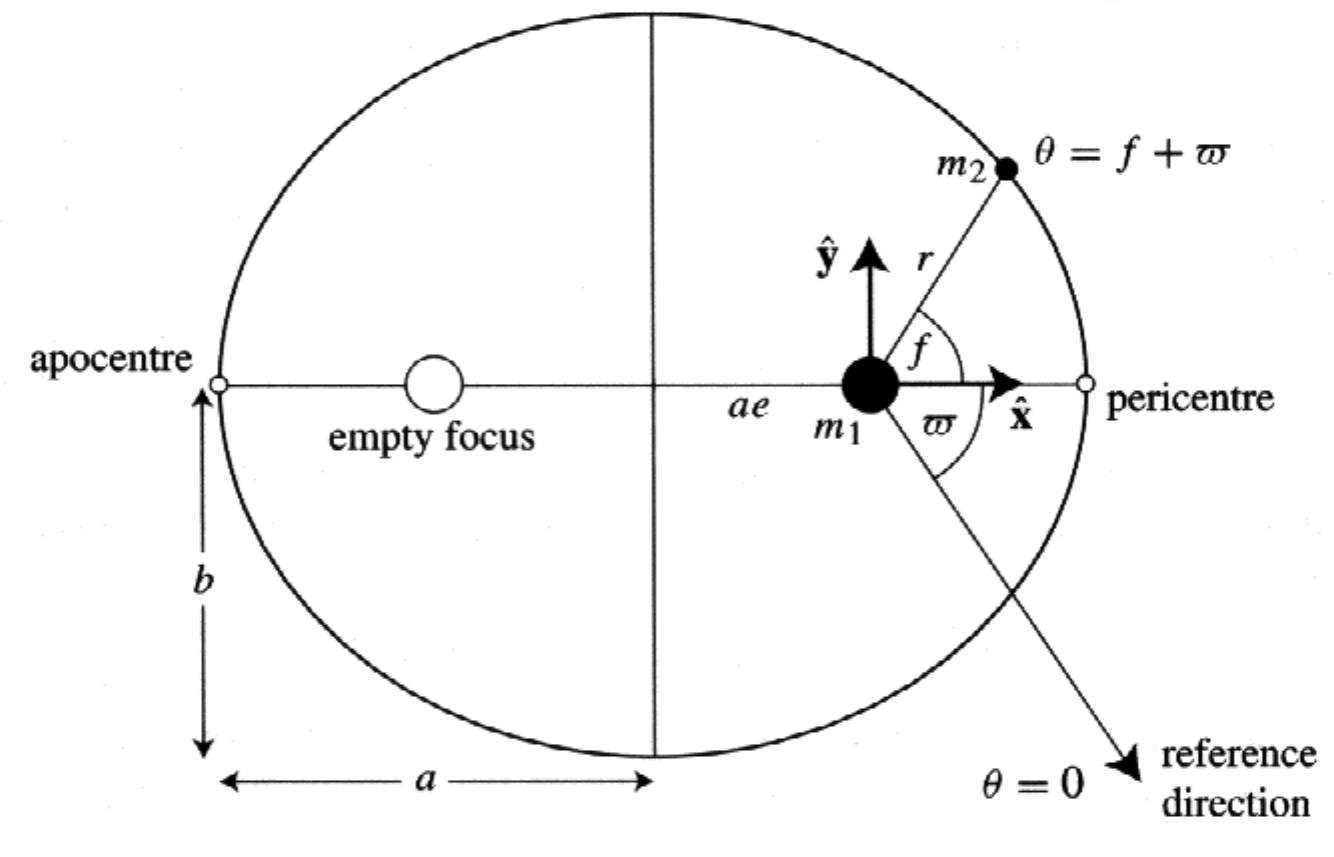
\includegraphics[width=\linewidth]{gfx/ellipse.pdf}
    \caption[Elliptical orbit.]{An elliptical orbit. The mass $m_1$ sits in one focus and $m_2$ orbits 
    around it. The position  of $m_2$ on the ellipse is specified by two angles, 
    the true anomaly $f$ and the argument of pericentre $\omega$. Only $f$ 
    varies in the two--body problem, $\omega$ stays fixed in the absence of an
    external perturbation.} 
\label{fig:ellipse}
\end{figure}
\Cref{fig:ellipse} shows an elliptical orbit in two dimensional space. The mass
$m_2$ orbits around $m_1$ which is located in one of the foci of the ellipse.
The position of $m_2$ at each moment in time is described by the $2\pi$--periodic
angle 
$f=\theta - \omega$ called the \emph{true anomaly}. The angle $\omega$ is specified 
relative to an arbitrary reference direction and it is constant throughout the 
motion. $f=0$ corresponds to the closest approach of $m_2$ to $m_1$ which 
happens at a point in orbit called 
the \emph{pericentre}. Conversely, the point furthest away from 
$m_2$ at $f=\pi$ is called the \emph{apocentre} . 
The \emph{semi-major axis} of the ellipse $a$ is given by
\begin{equation}
    a= \frac{h^2}{\mu} \frac{1+e}{1-e} 
\end{equation}
One can easily derive \citep[ex.][]{murray} \emph{Kepler's third law}, given by
\begin{equation}
    T^2= \frac{4\pi^2}{\mu} a^3
    \label{eq:kepler_law}
\end{equation}
where $T$ is the orbital period of $m_2$ around $m_1$. We also define the so-called
\emph{mean motion} $n$, as
\begin{equation}
    n= \frac{2\pi}{T} 
\end{equation}
The mean motion is the average angular frequency of the periodic motion; it is 
constant in the two--body problem but in general varies when additional bodies are 
present.

If we multiply \cref{eq:4} by $\dot{\vect{r}}$ and use the expressions for
$\dot{\vect{r}}$ and $\ddot{\vect{r}}$ from \cref{eq:9}, we obtain the following
constant of motion
\begin{equation}
    \frac{1}{2} v^2 - \frac{\mu}{r} =C
\end{equation}
where $v^2=\dot{\vect{r}}\cdot\dot{\vect{r}}$ is velocity squared and $C$ is a
constant of motion, the energy per unit mass. It can be shown \citep{murray}
that $C$ is given by
\begin{equation}
    C= -\frac{\mu}{2a} 
\end{equation}
thus, the energy of a closed orbit in the two--body problem depends only on the semi-major axis.
\subsection{The mean and eccentric anomaly}
By solving the orbit equation, we have established that the mass $m_2$ orbits 
around $m_1$ in an ellipse if $e<1$. However, it is not immediately clear how
to explicitly solve for the time dependence of $r$ and $f$ and thus determine 
the position of $m_2$ at any given time, because $f$ and $r$ vary
non-linearly with time for $e\neq 0$. For reasons which will become apparent 
later, we would like to construct an angle which varies linearly with time.
One such angle is the \emph{mean anomaly} $M$ defined as
\begin{equation}
    M=n(t-\tau)
\label{eq:mean_anomaly}
\end{equation}
where $\tau$ is the \emph{time of pericentre passage} -- time elapsed
since the orbiting body was at pericentre, and it is constant. $M$
increases linearly with time at a rate equal to the mean motion. At $t=\tau$ 
we have $M=f=0$
and at $t=\tau + T/2$ $M=f=\pi$, thus, at the pericentre and apocentre 
M matches with $f$. The angle $M$ has no obvious geometrical significance
but we can define another angle which does. \Cref{fig:eccentric_anomaly} 
shows the orbital ellipse with semi-major axis $a$ together with a 
circumscribed circle of radius $a$ concentric with the ellipse. A line 
perpendicular to the semi-major axis of the ellipse intersects two points,
one on the orbit and one on the circumscribed circle. We define the 
\emph{eccentric anomaly} $E$ to be the angle between the semi-major axis
of the ellipse and the intersected point on the circle. Again, we have
$E=M=0$ at $f=0$ and $E=M=\pi$ at $f=\pi$. 
\begin{figure}[htb]
\centering
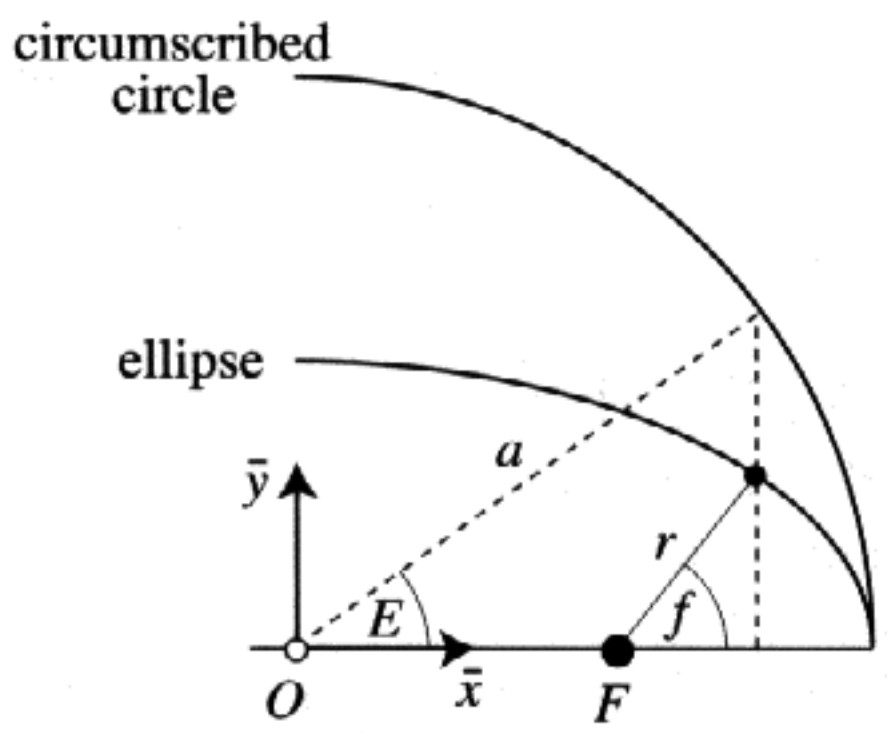
\includegraphics[width=0.5\linewidth]{gfx/eccentric_anomaly.png}
    \caption[Eccentric anomaly.]{A geometrical description of 
    the eccentric anomaly $E$. Figure from \citet{murray}.}
\label{fig:eccentric_anomaly}
\end{figure}
From geometry one can show that the following relation between the
angles $f$ and $E$ is satisfied
\begin{equation}
    \cos f= \frac{\cos E -e}{1-e\cos E} 
    \label{eq:eccentric_anomaly}
\end{equation}
Thus, there is a one-to-one correspondence between $f$ and $E$ as long as
both are measured with respect to the positive $x$ axis. To 
locate the location of the body on its orbit at time $t$, we need
a relationship between $E$ and $M$. This relation ship is called
the \emph{Kepler's equation} and is given by \citep{murray}
\begin{equation}
    M=E-e\sin E
    \label{eq:kepler_equation}
\end{equation}
A solution to this equation enables us to locate the body on its orbit
at any given time. The procedure is as follows
\begin{enumerate}
    \item At a particular time $t$ find $M$ from \cref{eq:mean_anomaly}
    \item Solve the Kepler's equation for $E$
    \item Use \cref{eq:eccentric_anomaly} to find $f$
\end{enumerate}
Kepler's equation is transcendental in $E$ and therefore it cannot
be solved directly. 

Finally, we define one last angle $\lambda$ called the
\emph{mean longitude} as
\begin{equation}
    \lambda =M +\omega
\end{equation}
Since it is derived from $M$, it does not have a geometrical 
interpretation. All longitudes are defined with respect to a 
common, arbitrary reference point.
\subsection{Orbit in an inertial frame}
So far we have derived a solution for the \emph{relative} motion
of $m_2$ with respect to $m_1$, we now turn to the description of the
orbit in a non-accelerating \emph{inertial frame}.
\begin{figure}[htb]
\centering
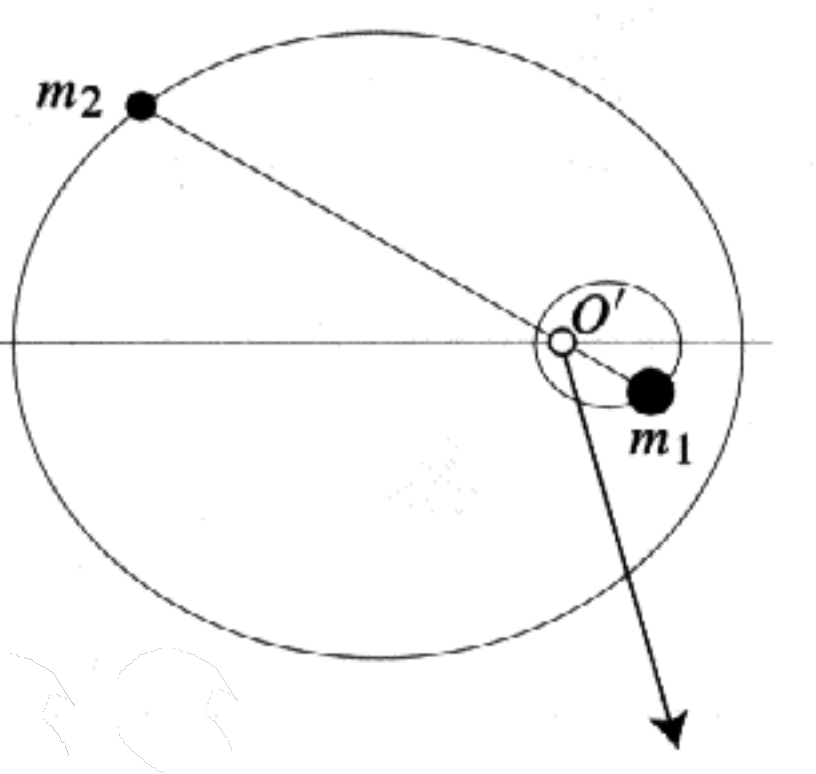
\includegraphics[width=0.5\linewidth]{gfx/barycentric_orbit.pdf}
    \caption[Barycentric orbit.]{The motion of $m_2$ and $m_1$ 
    with respect to their centre
    of mass $O'$.}
\label{fig:barycentric_orbit}
\end{figure}
It is not difficult to show that the masses $m_1$ and $m_2$ again
orbit in a conic section around their centre of mass with the same
period $T$ as before. 
\Cref{fig:barycentric_orbit} shows the orbits with respect to the
centre of mass. We need not worry about the motion of the centre
of mass itself because of a result from elementary mechanics which says
that the centre of mass of a collection of particles always moves at
constant velocity in a straight line and is therefore a valid inertial
reference frame. The conic sections of the orbits relative to the centre
of mass are 
reduced in scale by mass factors, as follows
\begin{equation}
    a_1= \frac{m_2}{m_1 + m_2} a\quad a_2= \frac{m_1}{m_1 + m_2} a
\end{equation}
where $a_1$ is the semi-major axis of the orbit of $m_1$ around $O'$
and $a_2$ is the semi-major axis of the orbit of $m_2$ around $O'$.

The \emph{total} angular momentum of the system is given by 
\begin{equation}
    L= \frac{m_1 m_2}{m_1 + m_2} \sqrt{\mu a(1-e^2)}
    \label{eq:ang_momentum}
\end{equation}
and the total orbital energy is
\begin{equation}
    E= -G \frac{m_1 m_2}{2a} 
\end{equation}
The energy of a Keplerian orbit depends only on the semi-major axis
and the angular momentum depends on both the semi-major axis and
the eccentricity. In particular, if the semi-major axis is constant
the only way to change the eccentricity is by changing the angular
momentum. This simple fact is the essence of so-called secular
interactions described in \cref{sec:three_body}. The angular momentum
is largest for a circular orbit.

\subsection{Orbit in three-dimensional space}
We have determined that the bodies in the two--body problem move on
on an ellipse in inertial space. The orientation of that ellipse 
stays fixed for all time if no external bodies are present. If there 
are other bodies in the system however, the orbit no longer stays
fixed, both its shape and orientation change in three-dimensional space.
Because of that, it is useful to define the orientation of the orbit
in 3D space relative to a fixed reference plane.
\begin{figure}[htb]
\centering
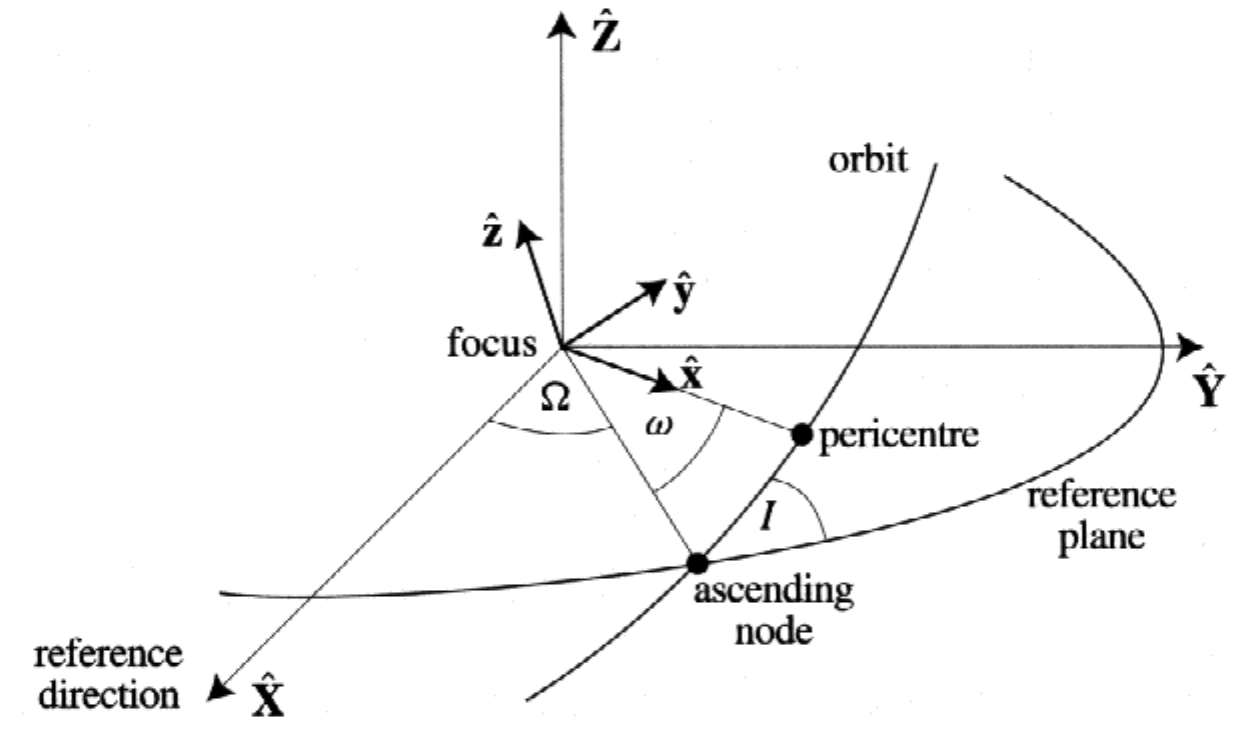
\includegraphics[width=0.8\linewidth]{gfx/3d_orbit.png}
    \caption[Orbit in 3D space.]{A Keplerian orbit in 3D space, figure
    from \citet{murray}.}
\label{fig:3d_orbit}
\end{figure}
\Cref{fig:3d_orbit} shows the orbit in 3D Cartesian coordinate system,
the reference plane is taken to be the $X-Y$ plane. The orbital
ellipse intersects the reference plane in two points, in order to define
its orientation relative to fixed axes we have to choose one. Independent
on wheater the orbiting body is moving around the ellipse in a clockwise
or counter-clockwise direction, the body will pass through the reference
plane \emph{from below} (where below means the $-Z$ direction)
at one of the two points. We call this point the \emph{ascending node}
and choose it as a reference. The angle from the ascending node to the
$X$ axis is then called the \emph{longitude of the ascending node} and
is denoted by $\Omega$. The angle between the plane of the ellipse and
the reference plane is called the \emph{inclination} of the orbit and
is defined in the range $0\leq I\leq \pi$.

Thus, we have completely described the orbit in 3D space. However, it is useful to 
define another angle $\varpi$ called the \emph{longitude of pericentre.} 
$\varpi$ is not really a true angle since it is defined as a sum of 
angles in two separate planes. When the inclination is zero (the orbit
is co-planar with the reference plane) we have $\varpi=\omega$. 

It can be shown that each there is a one-to-one correspondence between 
a set of Cartesian positions and velocities $(x,y,z,v_x,v_y,v_z)$ 
of a given massive particle and an \emph{instantaneous} Keplerian orbit 
defined by $(a,e,I,\Omega,\omega,f)$ with respect to another massive
particle. This is why it is still useful to talk about orbits even
when we are dealing with a system of multiple bodies. Although those
bodies won't stay on a fixed Keplerian orbit for all time, at any given
time we can still define an instantaneous Keplerian orbit.
Most bodies in stable systems change their orbital elements slowly
when exchanging energy and angular momentum with other bodies and
it is often more useful to use the orbital elements as a set of coordinates
instead of the Cartesian coordinates.

\section{A brief review of Hamiltonian mechanics}
\label{sec:hamiltonian_mechanics}
\subsection{Hamilton's equations}
\label{sub:Hamilton's equations}
The two--body problem could have been solved equally well using a different
formulation of mechanics called \emph{Hamiltonian mechanics}, named after
William Rowan Hamilton (1805--1865). Hamiltonian
mechanics is equivalent to Newtonian mechanics but is often more suitable
for certain types of problems, and the concept of a Hamiltonian function
is a lot more general than Newton's second law of mechanics.

In Newtonian mechanics the full description of a dynamical system 
consisting of N particles is 
obtained by solving a system of second order differential equations
of the form
\begin{equation}
    \dot{\vect{p}}_i=\vect{F}_i
\end{equation}
where $\dot{\vect{p}}_i=m_i\dot{\vect{r}}_i$ is the momentum of the
i-th particle, $m_i$ is its mass and $\vect{r}_i$ its position vector
relative to an origin of an inertial reference system. This 
constitutes a system of 3N second order differential equations for
the positions vectors $\vect{r}_i$.

In the Hamiltonian formalism a dynamical system is described by 
a function of \emph{generalized coordinates} $\vect{q}$ and \emph{momenta} 
$\vect{p}$ called the \emph{Hamiltonian} $\mathcal{H}(\vect{q},
\vect{p})$. Each pair $(q_i,p_i)$ constitutes a single 
\emph{degree of freedom}, it is said to be \emph{conjugate} . 
The time evolution of these coordinates and 
momenta
$(\vect{q},\vect{p})$, collectively known as the \emph{phase space},
is given by \emph{Hamilton's equations} 
\begin{equation}
    \dot{q}_i= \frac{\partial \mathcal{H}}{\partial p_i}\quad
    \dot{p}_i= -\frac{\partial \mathcal{H}}{\partial q_i} 
    \label{eq:hamiltons_equations}
\end{equation}
Instead of 3N second order differential equations for a system of N particles,
this is a system of
6N \emph{coupled first-ordered} equations. Once the initial conditions
$(\vect{q}_0,\vect{p}_0)$ are specified, the solution of Hamilton's 
equations defines a \emph{unique} trajectory in a 
6N dimensional phase space. The coordinate pair $(\vect{q},\vect{p})$
is said to be \emph{canonical} if the coordinates satisfy 
Hamilton's equations. The main advantage of the Hamiltonian
formalism compared to other formalisms of mechanics is the ability
to easily transform to different choices of $(\vect{q},\vect{p})$.
as long as the new set of coordinates is also canonical. There are no
other strict requirements on the new coordinates, the momentum 
$p_i$ coincides with the real momentum $m_i \dot{q}_i$ only in
Cartesian coordinates.

We can arbitrarily scale the momentum and the coordinate by a 
constant factor, for example $p\rightarrow\eta p\quad q\rightarrow\nu q$, 
, as long as we also
rescale the time. This can be seen from the form of 
\cref{eq:hamiltons_equations} because
\begin{equation}
    \frac{\partial \mathcal{H}}{\partial (\eta p)}= 
    \frac{\mathrm{d}q}{\mathrm{d}(\eta t)}  
    \label{eq:rescaling_hamiltonian}
\end{equation}
and similarly for the coordinate scaling. Transformations of this
type are known as \emph{scale transformations} and they are simply 
a reflection of the fact that the equations of motion should be invariant
to the changes of units.
\subsection{Integrable Hamiltonians}
The Hamiltonian formalism is useful for finding conserved quantities.
If a generalized coordinate $q_i$ does not appear in the Hamiltonian
the corresponding momentum conjugate $p_i$ is a conserved quantity
\begin{equation}
    \dot{p}_i= \frac{\partial \mathcal{H}}{\partial q_i} =0
\end{equation}
If the motion is in a fixed potential, the Hamiltonian is equal
to the total energy of the system $E$.

If a particular Hamiltonian $\mathcal{H}$ can be reduced to a form
where it depends only on the momenta, that is
\begin{equation}
    \mathcal{H}(\vect{p})
\end{equation}
then the momenta $\vect{p}$ are conserved and the system is said to be
\emph{integrable}. An integrable system with $n$ degrees of freedom
has $n$ constants of motion. From Hamilton's equations, it follows that the time
evolution of the coordinates is simply
\begin{equation}
    \dot{q}_i= \frac{\partial \mathcal{H}}{\partial p_i} =\omega_i
\end{equation}
that is, all of the coordinates evolve linearly in time with constant
frequencies $\omega_i$ which depend only on the momenta
\begin{equation}
q_i(t)=\omega_i t
\end{equation}
Integrable systems are very rare  in the space of all Hamiltonians and 
it is not immediately clear
if a given Hamiltonian can be reduced to an integrable form.

Systems of the form
\begin{equation}
    \mathcal{H}=\mathcal{H}_0(\vect{p})+\epsilon \mathcal{H}_1(\vect{q})
\end{equation}
where $\mathcal{H}_0$ is an integrable Hamiltonian, $\mathcal{H}_0$ is 
a perturbation and $\epsilon$ is a small parameter are said to be nearly 
integrable
and in general they display chaotic behaviour. However, if $\epsilon$ is 
small enough most solutions still lie in the region of phase space
allowed by the solutions of $\mathcal{H}_0$.

Systems with a single degree of freedom are always integrable and
the Hamiltonian itself is a conserved quantity (i.e. the energy
is conserved). The trajectory is defined completely by the value
of energy. They are often used as an approximation for a generally
more complex system. Obtaining a single degree of freedom
Hamiltonian for a resonance is a major goal of
\cref{ch:analytical_model}.

The Keplerian Hamiltonian for the two--body problem is completely 
integrable and it can be written as
\begin{equation}
    \mathcal{H}_k=- \frac{\mu^2\mu^*}{2\Lambda^2} 
\end{equation}
where $\mu^*=m_1m_2/(m_1+m_2)$ and $\Lambda$ is the generalized
momentum conjugate to the orbital element coordinate $\lambda$,
the mean anomaly. The original Keplerian Hamiltonian has 6 
degrees of freedom. The conservation of \emph{total} linear and total
angular momentum vectors and the conservation of total energy
give 7 constants of motion. There is also a hidden symmetry in
the problem that we haven't mentioned previously. One can show that
one of the three components of the 
\emph{Runge-Lenz} vector is also a constant of motion, which 
bring the total to 8. The Runge-Lenz vector is a vector pointing
in the direction of periastron, defined by
\begin{equation}
    \vect{e}=\dot{\vect{r}}\times(\vect{r}\times\dot{\vect{r}})
    /(G(m_1+m_2)) - \vect{\hat r}
\end{equation}
Its magnitude is equal to the eccentricity of the orbit. We 
see that the number of constants of motion over-determines the 
problem. In fact, the two extra constants of motion are responsible
for the fact that that the relative motion is not only restricted to 
a conic curve, but it is also a conic section in the inertial
(centre of mass) frame. Because of this the orbit is also fixed in
3D space.

\subsection{Fixed points}
Given a Hamiltonian $\mathcal{H}(q,p)$ with a single degree of freedom
its \emph{fixed points}, points which do not move under time evolution,
are solutions of
\begin{equation}
    \dot{p}=0\quad\dot{q}=0
\end{equation}
From 
Hamilton's equations, it follows that their location is given by
\begin{equation}
   \frac{\partial \mathcal{H}}{\partial p}= \frac{\partial \mathcal{H}}{\partial q}=0
\end{equation}
Given a fixed point $(q_0,p_0)$, it is useful to derive the equations
of motion in its vicinity. If a test particle in its vicinity moves 
on a trajectory away from the fixed point, the point is said to be
\emph{unstable}. Conversely, if it remains near the fixed point for all 
time, the point is said to be \emph{stable}. We can expand the Hamiltonian
near the fixed point in a Taylor series
\begin{align}
    \mathcal{H}(\tilde q, \tilde p)=\mathcal{H}(q_0,p_0) 
    + \frac{\partial^2\mathcal{H}(q_0,p_0)}{\partial q^2} \frac{\tilde q^2}{2} 
    &+\frac{\partial^2\mathcal{H}(q_0,p_0)}{\partial p^2} \frac{\tilde p^2}{2} \nonumber\\
    &+\frac{\partial^2\mathcal{H}(q_0,p_0)}{\partial q\partial p}\tilde q\tilde p 
\end{align}
where $\tilde q=q-q_0$ and $\tilde p=p-p_0$. We can write this more succinctly 
in vectorial form as
\begin{equation}
    \mathcal{H}(\tilde q,\tilde p)= \frac{1}{2} \vect{x}^\tau\vect{M}\vect{x}
\end{equation}
where $\vect{x}=(\tilde q, \tilde p)$ and $\tau$ denotes the transpose 
operation. $\vect{M}$ is called the \emph{Hessian matrix} and is given by
\begin{equation}
    \vect{M}=
    \begin{pmatrix}
        \frac{\partial^2 \mathcal{H}}{\partial q^2} &
        \frac{\partial^2 \mathcal{H}}{\partial q\partial p }\\
        \frac{\partial^2 \mathcal{H}}{\partial p \partial q} &
        \frac{\partial^2 \mathcal{H}}{\partial p^2} 
    \end{pmatrix}
    \label{eq:fixed_points_stability}
\end{equation}
it is evaluated at the fixed points $(q_0,p_0)$.
It is symmetric and therefore has two real 
eigenvalues and two eigenvectors. It can be shown that after 
diagonalizing this matrix, the Hamiltonian assumes the form
\begin{equation}
    \mathcal{H}(q,p)= \frac{1}{2} (\lambda_1 q^2 + \lambda_2 p^2)
\end{equation}
where $\lambda_1$ and $\lambda_2$ are the eigenvalues. If the
eigenvalues are both negative or both positive (i.e. the
determinant is positive) the system undergoes
harmonic oscillations (librations) about the fixed point with 
frequency
\begin{equation}
    \omega = \sqrt{\lambda_1\lambda_2}
\end{equation}
and we say the fixed point is a \emph{center}. If one of the 
eigenvalues is negative and the other positive (the determinant
is negative) the system is
diverging exponentially away from the fixed point in the 
direction of one \emph{eigenvector} and heading towards the 
fixed point along the direction of the other eigenvector. The
fixed point is unstable and we call it a \emph{saddle}.

\subsection{Canonical transformations}
\label{sub:Canonical transformations}
A \emph{canonical transformation} is a coordinate transformation
from a set $(\vect{q},\vect{p})$ to $\left[Q(\vect{q},\vect{p}),
P(\vect{q},\vect{p})\right]$ which preserves the form of Hamilton's
equations. It can be shown that canonical transformations
satisfy the Poisson brackets
\begin{equation}
    \{P_i,P_j\}=0\quad\{Q_i,Q_j\}=0\quad\{Q_i,P_j\}=\delta_{i,j}
\end{equation}
where $\delta_{i,j}$ is the \emph{Kronecker delta} symbol and
the Poisson bracket is defined as
\begin{equation}
    \{f,g\}=\sum^N_{i=0}\left( \frac{\partial f}{\partial q_i} 
    \frac{\partial g}{\partial p_i} -\frac{\partial f}{\partial p_i} 
    \frac{\partial g}{\partial q_i} \right)
\end{equation}
where the sum goes over all the degrees of freedom. The question remains 
how to easily construct transformations which are canonical. The
answer lies in the form of \emph{generating functions}. Consider
a function $F_1(q,Q)$ of the old and new coordinates and let
\begin{equation}
    p_i= \frac{\partial F_1}{\partial q_i} 
\end{equation}
After inverting, this equation defines a new coordinate $Q_i=Q_i(q,p)$.
One can show that the new momentum is then given by
\begin{equation}
    P_i=- \frac{\partial F_1}{\partial Q_i} 
\end{equation}
Thus we have found a way to construct a canonical transformation to new
coordinates. We can choose the new coordinates $Q_i$, however, the requirement 
that the new coordinates form a conjugate pair restricts our freedom
to choose the new momentum as well. The function $F_1(q,Q)$ is called
the \emph{generating function of first kind} . There are three additional
kinds of generating functions, the possibilities are listed in 
\cref{tab:generating_functions}.
\begin{table}[h!]
\centering
\begin{tabular}{cll}
\toprule
    Generating function &\multicolumn{2}{c}{Derivatives}\\
\midrule
    $F_1(q,Q)$ & $p_i=\frac{\partial F_1}{\partial Q_i}$ & 
    $P_i=\frac{\partial F_1}{\partial q_i}$\\
    $F_2(q,P)$ & $p_i=\frac{\partial F_2}{\partial q_i}$ & 
    $Q_i=\frac{\partial F_2}{\partial P_i}$\\
    $F_3(p,Q)$ & $q_i=-\frac{\partial F_3}{\partial p_i}$ & 
    $P_i=-\frac{\partial F_3}{\partial Q_i}$\\
    $F_4(p,P)$ & $q_i=-\frac{\partial F_4}{\partial p_i}$ & 
    $Q_i=\frac{\partial F_4}{\partial P_i}$\\
\bottomrule
\end{tabular}
\caption{Different kinds of generating functions.}
\label{tab:generating_functions}
\end{table}
Which kind of the generating function is the best depends on the
problem at hand.

\section{The pendulum}
\label{sec:pendulum}
A simple single degree of freedom Hamiltonian useful for the study
of resonance is that of the pendulum. The Hamiltonian has the form
\begin{equation}
    \mathcal{H}(\phi,p)= \frac{1}{2} p^2 -\omega_0^2\cos\phi
\end{equation}
Where $\omega_0$ has dimensions of frequency. By solving 
Hamilton's equations, we obtain
\begin{align}
    \dot{\phi} &= p\\
    \dot{p} &= - \omega_0^2\sin\phi
\end{align}
Combining the two equations, we obtain a single equation of motion
\begin{equation}
    \ddot{\phi}+\omega_0^2\sin\phi =0
\end{equation}
We see that in the limit of small $\phi$ the motion is equivalent to
that of the harmonic oscillator oscillating with the frequency
$\omega_0$. The fixed points are located at
$(\phi, p)=(\pm k\pi,0)$ (where k is an integer) and there is 
a single 
stable center point located at $(\phi¸ p)=(\pi, 0)$. It is 
sufficient to study the two fixed points $(0,0)$ and $(\pi,0)$
since the motion is periodic. For the fixed point at $(0,0)$, we have
\begin{equation}
    \vect{M}=
    \begin{pmatrix}
        1 & 0\\
        0 & -\omega_0^2 
    \end{pmatrix}
\end{equation}
and we see that this point is a stable center. For the other point 
at $(\pi,0)$, we have
\begin{equation}
    \vect{M}=
    \begin{pmatrix}
        \omega_0^2 & 0\\
        0 & 1
    \end{pmatrix}
\end{equation}
The point is an unstable saddle point.
\begin{figure}[htb]
\centering
\includegraphics[width=\linewidth]{gfx/pendulum.pdf}
    \caption[Pendulum phase space portrait.]{The phase space of a pendulum. 
    The red curve denotes the 
    separatrix filled circles denote stable fixed points, open circles denote
    unstable fixed points.}
\label{fig:pendulum}
\end{figure}
\Cref{fig:pendulum} shows the level curves (curves of constant $\mathcal{H}$)
of the pendulum. Given a specific value of the energy, the system stays 
on one of the curves for all time. The motion around the fixed point $(0,0)$
 in between the fixed points at $-\pi$ and $\pi$ is said to be \emph{libratory}.
There is also an entirely different type of motion where $\phi$ is unbounded,
these trajectories are called \emph{circulatory}. The curve which passes through
the unstable points separates the two regimes and is called the \emph{separatrix.} 
As seen from the figure\footnote{This can also be shown rigorously by deriving the
expression for $\omega_{lib}$ as a function of maximum $\phi$.},
the oscillation period increases from the initial
small amplitude value of $2\pi/\omega_0$ to infinity as the separatrix is
approached. Once the separatrix is crossed the motion is unbounded. This
steep dependence of the librational period on the distance to the separatrix is
responsible for chaos in weakly interacting non-linear systems (see
\citet{cambridgenbody} for a broader discussion of this point). The concepts
presented in this section will be important for the study of resonance in the
three--body problem.

\section{The three--body problem}
\label{sec:three_body}
\subsection{The disturbing function}
Finally, we move to the problem of three gravitationally interacting massive 
bodies, such as the circumbinary system consisting of two stars and 
an outer planet. The three--body problem is famously not integrable, many 
great mathematicians such as Newton and Poincaré have tried and failed to find and
exact solution. However, it is still possible to do a perturbative analysis
in the case when one of the bodies is only weakly interacting with the
other two. The following discussion largely follows \citett{Mardling2013}.

A stable hierarchical system of three bodies naturally divides into
two orbits composed of an "inner binary" and an "outer binary". We will work
in \emph{Jacobi coordinates} which are defined such that in a hierarchical
system consisting of $N$ bodies, the $N$th body is defined in a coordinate 
system whose origin is the centre of mass of the previous $N-1$ bodies. 
\Cref{fig:jacobi} shows a system of three masses $m_1$, $m_2$ and $m_3$ in
Jacobi coordinates. The position vector $\vect{r}$ points from $m_1$ to $m_2$ 
and it is the same vector as in our previous analysis of the two--body 
problem. The position vector $\vect{R}$ points from the centre of mass
of the inner binary consisting of $m_1$ and $m_2$ to the outer mass $m_3$.
Thus, at any given moment we can define two Keplerian orbits, one for
the inner binary and one for the outer binary. Since the three--body
problem is not integrable the orbits will in general no longer be fixed
and will change their orbital elements with time. This choice of coordinates
obviously fails in the case of crossing orbits since the hierarchy loses
its meaning, however, a system with crossing orbits is inherently unstable
and not the subject of our interest.
\begin{figure}[htb]
\centering
\includegraphics[width=\linewidth]{gfx/jacobi.pdf}
    \caption[Jacobi coordinates.]{A system of three massive 
    bodies in Jacobi coordinates. 
    The point $C_{12}$ denotes the centre of mass of the inner two 
    bodies and the point $C_{123}$ that of the whole system.}
\label{fig:jacobi}
\end{figure}

When the system is stable the inner and outer orbits interact only 
weakly by means of an interacting potential called the 
\emph{disturbing function}. The disturbing function can be written
as an infinite Fourier series of angles called the \emph{harmonic
angles} (or sometimes resonance angles), it is responsible 
for the exchange of energy and angular 
momentum between the two orbits.  Each resonance angle is a linear
superposition of all angles in the system. A resonance angles can either 
circulate or librate in exactly the same way as the angle in the pendulum model
described in the previous section.
If a particular resonance angle is librating, we say that the system
is in \emph{resonance}. The various resonance angles can mutually 
interact, under certain conditions a system can exist in two 
neighbouring resonant states where two resonant angles librate 
at a similar period. This is known as \emph{resonance overlap} 
and it leads to chaotic behaviour as the resonance angle approaches
the unstable fixed points \citep{WalkerFord1969}. The resonance
overlap criterion is then a good indication of whether the
system is chaotic or not.

We can write the equations of motions as
\begin{equation}
\begin{aligned}
    m_1\ddot{\vect{r}}_1&= \frac{Gm_1m_2}{r^2_{12}} \vect{\hat r}_{12}+
    \frac{Gm_1m_3}{r^2_{13}} \vect{\hat r}_{13}\\
    m_2\ddot{\vect{r}}_2&= -\frac{Gm_1m_2}{r^2_{12}} \vect{\hat r}_{12}+
    \frac{Gm_2m_3}{r^2_{23}} \vect{\hat r}_{23}\\
    m_3\ddot{\vect{r}}_3&= -\frac{Gm_1m_3}{r^2_{13}} \vect{\hat r}_{13}-
    \frac{Gm_2m_3}{r^2_{23}} \vect{\hat r}_{23}
\label{eq:three_body_newton}
\end{aligned}
\end{equation}
where the position vectors $r_i$ point from the centre of mass of 
system $C_{123}$ to the mass $m_i$ and $\vect{r}_{ij}=\vect{r}_j-\vect{r}_i$. 
\Cref{eq:three_body_newton} constitutes a system with 9 degrees of freedom.
Again we have the 7 conserved quantities due to momentum and energy 
conservation, however, there is no analogue of the Runge-Lenz vector
in the three--body problem. Therefore, the system is not completely
integrable, in fact, it admits \emph{chaotic} solutions -- solutions which
are extremely sensitive to small variations in the initial conditions. 
There are two kinds of stability, one is called \emph{Lagrange stability} 
and the other \emph{Hill stability}. The latter happens due to close
approaches of two bodies which most often result in an ejection of one
of the bodies, and the former does not require close approaches.
In this chapter we are primarily interested in Lagrange instability 
because scattering events are difficult to handle analytically
and only become important after the onset of Lagrange instability in 
circumbinary systems. 

We start by rewriting \cref{eq:three_body_newton} in Jacobi coordinates
and define the vectors $\vect{r}=\vect{r}_2-\vect{r}_1$ and 
$\vect{R}= (m_{123}/m_{12})\vect{r}_3$.
We can now rewrite \cref{eq:three_body_newton} as
\begin{equation}
\begin{aligned}
    \mu_i\ddot{\vect{r}}+ \frac{Gm_1m_2}{r^2} \vect{\hat r}&= \frac{
        \partial \mathcal{R}}{\partial \vect{r}} \\
    \mu_o\ddot{\vect{R}}+ \frac{Gm_{12}m_3}{R^2} \vect{\hat R}&= \frac{
        \partial \mathcal{R}}{\partial \vect{R}} 
    \label{eq:three_body_newton_R}
\end{aligned}
\end{equation}
where $R=\lvert\vect{R}\rvert$, $\mu_i=m_1m_2/m_{12}$ and $\mu_o=m_{12}m_3/m_{123}$
and
\begin{equation}
    \mathcal{R}=- \frac{Gm_{12}m_3}{R} + \frac{Gm_2m_3}{\lvert\vect{R}-\beta_1\vect{r}
    \rvert} + \frac{Gm_1m_3}{\lvert\vect{R}+\beta_2\vect{r}\rvert}
    \label{eq:dist_cartesian}
\end{equation}
is the disturbing function with $\beta_i=m_i/m_{12},\,i=1,2$. We use the subscripts
$i$ and $o$ to denote quantities defined with respect to the inner and outer orbits
respectively. The notation $\partial/\partial\vect{r}$ refers to the gradient with 
respect to the spherical polar coordinates $(r,\theta_1,\phi_1)$ 
associated with the position od body 2 relative to the centre of mass $C_{12}$, similarly,
$\partial/\partial\vect{R}$ is the gradient associated with the position 
of body 3 with coordinates $(R,\theta_o,\phi_o)$
relative to the same origin. All information
about the mutual interaction of the inner and outer orbits is contained in
$\mathcal{R}$\footnote{Historically, most versions of the expanded disturbing
function have units of energy per unit mass. The expansion presented in RM2013 has
units of energy}. In the limit when the inner two masses coalesce ($r/R\rightarrow 0$)
or the mass ratio between the planet mass $m_3$ and the total binary mass $m_{12}$
goes to zero ($m_3/m{12}\rightarrow 0$), $\mathcal{R}$ vanishes and the two orbits
no longer interact with each other. 

The total energy (or the Hamiltonian) is given by
\begin{equation}
    \mathcal{H}=\mathcal{H}_i+\mathcal{H}_o-\mathcal{R}
    \label{eq:three_body_hamiltonian}
\end{equation}
where
\begin{equation}
    \mathcal{H}_i= \frac{1}{2}\mu_i\dot{\vect{r}}\cdot\dot{\vect{r}}- \frac{Gm_1m_2}{r}, \quad
    \mathcal{H}_o= \frac{1}{2}\mu_o\dot{\vect{R}}\cdot\dot{\vect{R}}- \frac{Gm_{12}m_3}{R}
\end{equation}
are the Keplerian Hamiltonians corresponding to the inner and outer orbits and the 
disturbing function has a role of interaction energy. The two Keplerian Hamiltonians
individually are fully integrable as mentioned previously, the complete Hamiltonian
is not. 

Given 
\cref{eq:three_body_hamiltonian}, one can calculate the Hamilton's equations of
motion. Those are equivalent to \cref{eq:three_body_newton_R}, except that they
are first order in time. If those equations are then expressed in terms
of the inner and outer orbital elements, they are called 
\emph{Lagrange's planetary equations}. The derivation is presented
in \citet[for ex.][]{brouwer1961}, here we merely state the result for coplanar
systems
\begin{equation}
\begin{aligned}
    \dot{e}&= -\frac{s(1-s)}{\mu na^2e} 
    \frac{\partial\mathcal{R}}{\partial\lambda}
    -\frac{s}{\mu na^2e} 
    \frac{\partial\mathcal{R}}{\partial\varpi}\\
    \dot{\varpi}&= \frac{s}{\mu na^2e} 
    \frac{\partial\mathcal{R}}{\partial e}\\
    \dot{\epsilon}&=- \frac{2}{\mu n a} 
    \frac{\partial\mathcal{R}}{\partial a}
   +\frac{s(1-s)}{\mu na^2e} 
    \frac{\partial\mathcal{R}}{\partial e} 
\end{aligned}
    \label{eq:lagrange_planetary_equations}
\end{equation}
where the subscripts of the orbital elements are either $i$
or $o$ for the inner and outer orbits respectively. $s=\sqrt{1-e^2}$
and $\epsilon$ is the mean longitude at $t=t_0$ and is related
to the mean longitude by $\int^t_0 n\mathrm{d}t$ 
\citep[see.][for details]{Mardling2013}. There is no unique general 
solution for \cref{eq:lagrange_planetary_equations}, best one can do
is to expand $\mathcal{R}$ in a series and consider a few dominant
terms in certain cases.

We start by expanding the last two terms in \cref{eq:dist_cartesian} using 
a well known\footnote{Expressions involving a difference between two vectors 
such as $1/\lvert \vect{r}-\vect{r}'\rvert$ occur in all kinds of problems 
in physics.} expansion in terms of \emph{spherical harmonics}. 
\begin{equation}
    \frac{1}{\lvert \vect{R} -\beta_s\vect{r}\rvert}= \frac{1}{R} \sum^\infty_{l=0}
  \frac{4\pi}{2l+1}   \left( \frac{\beta_s r}{R} \right)^l
    \sum^l_{m=-l} Y_{lm}(\theta_i,\phi_i)
    Y_{lm}^*(\theta_o,\phi_o)
    \label{eq:addition_theorem}
\end{equation}
$Y_{lm}$ is a spherical harmonic\footnote{Spherical harmonics are special
functions which form a complete set of orthogonal functions on the sphere, 
any function defined in terms of spherical polar coordinates can be expanded
in an infinite series of spherical harmonics as $f(\theta,\phi)
=\sum^\infty_{l=0}\sum^l_{m=-l}f^m_lY_l^m(\theta,\phi)$. The series converges 
if the coefficients $f^l_m$ decay in $l$ sufficiently rapidly.} of
\emph{degree l} and \emph{order m} with
$Y_{lm}^*$ being its complex conjugate. Using 
\cref{eq:addition_theorem} the disturbing function $\mathcal{R}$ becomes
\begin{equation}
    \mathcal{R}=G\mu_im_3\sum^\infty_{l=2}\sum^l_{m=-l}\left( \frac{4\pi}{2l+1} 
    \right)\mathcal{M}_l\left( \frac{r^l}{R^{l+1}} \right) Y_{lm}(\theta_i,\phi_i)
    Y_{lm}^*(\theta_o,\phi_o)
\label{eq:dist_harmonics}
\end{equation}
where $\mathcal{M}_l$ is a mass factor given by
\begin{equation}
    \mathcal{M}_l= \frac{m_1^{l-1}+(-1)^lm_2^{l-1}}{m_{12}^{l-1}} 
\end{equation}
\Cref{eq:dist_harmonics} is a spherical harmonic expansion with 
coefficients proportional to $(r/R)^l$. In order for this series
to converge, we require that $r/R$ be a small number. This is satisfied
for all CB planets because, as will be shown later, there is
an inner instability region just outside of the stellar binary and the only
stable orbits exist further outside the stellar binary's orbit. A spherical
harmonic is defined by
\begin{equation}
    Y_{lm}(\theta,\phi)=\sqrt{ \frac{2l+1}{4\pi} \frac{(l-m)!}{(l+m)!} }\mathcal{P}_1^m(
    \cos\theta)e^{im\phi}
    \label{eq:sph_harmonics}
\end{equation}
where $\mathcal{P}_1^m(\theta, \phi)$ is the \emph{associated Legendre function}
\citep{jackson}. 

Next, we focus on coplanar systems
(mutual inclination between orbits is assumed to be zero) and thus we take
$\theta_i=\theta_o=\pi/2$ (the motion is restricted to the $x-y$ plane), 
$\phi_i=f_i+\varpi_i$ and $\phi_o=f_o+\varpi_o$ where $f_i$ and $f_o$ are
the true anomalies of the outer and inner orbits respectively. We obtain 
\begin{equation}
    \mathcal{R}=g\mu_im_3\sum^\infty_{l=2}\sum^l_{m=-l,2} \frac{1}{2} c_{lm}^2\mathcal{M}_l
    e^{im(\varpi_i-\varpi_o)}\left(r^le^{imf_i}\right)\left( \frac{e^{-imf_o}}{R^{l+1}} 
    \right)
    \label{eq:dist_expanded}
\end{equation}
where
\begin{equation}
    c^2_{lm}= \frac{8\pi}{2l+1} \left[Y_{lm}(\pi/2,0)\right]=c^2_{l-m}
\end{equation}
and the notation $m=-l, 2$ in the summation over $m$ means that the summation is taken
in steps of 2. The first few values for $c_{lm}$ can be found in \citet{Mardling2013}.
For stable systems the expressions in the last two brackets of
\cref{eq:dist_expanded} are nearly periodic and can therefore be expanded in a 
\emph{Fourier series} of the inner and outer mean anomalies $M_i=n_it+M_i(0)$ and
$M_o=n_ot+M_o(0)$, where $n_i,n_o$ are the mean motions associated with the inner
and outer orbits and $M_i(0),M_o(0)$ are their values at $t=0$.  The result is
\begin{equation}
    r^le^{imf_i}\stackrel{\mathcal{F}}{=}a_i^l\sum^\infty_{n=-\infty}X^{l,m}_n(e_i)e^{inM_i}
    \label{eq:expansion_1}
\end{equation}
and
\begin{equation}
    \frac{r^{-imf_o}}{R^{l+1}} \stackrel{\mathcal{F}}{=}a_o^{-(l+1)}\sum^\infty_{n'=-\infty}
    X^{-(l+1),m}_{n'}(e_o)e^{-n'M_o}
    \label{eq:expansion_2}
\end{equation}
where the $\mathcal{F}$ above the equality sign denotes Fourier expansion 
and the \emph{Fourier coefficients} given by
\begin{equation}
    \begin{aligned}
        X^{l,m}_n(e_i)&= \frac{1}{2\pi} \int^{2\pi}_0 \left(\frac{r}{a_i}\right)^l
        e^{imf_i}e^{inM_i}\mathrm{d}M_i\\[4pt]
        &=\frac{1}{2\pi}\int^{2\pi}_0r^{l+1} e^{imf_i}e^{-inM_i}\mathrm{d}E_i
=    \mathcal{O}(e_i^{\lvert m-n\rvert})
    \label{eq:hansen_inner}
    \end{aligned}
\end{equation}
and
\begin{equation}
    \begin{aligned}
        X^{-(l+1),m}_{n'}(e_o)&= \frac{1}{2\pi} \int^{2\pi}_0 \left( \frac{R}{a_o}
        \right)^{-(l+1)}e^{-imf_o}e^{in'M_o}\mathrm{d}M_o\\[4pt]
        &=\frac{1}{2\pi}\int^{2\pi}_0R^{-l} e^{-imf_o}e^{in'M_o}\mathrm{d}E_o
        =\mathcal{O}(e_o^{\lvert m-n'\rvert})
    \end{aligned}
    \label{eq:hansen_outer}
\end{equation}
are called the \emph{Hansen coefficients}. The notation $\mathcal{O}()$
refers to the order of the leading terms. Plugging \cref{eq:expansion_1}
and \cref{eq:expansion_2} into \cref{eq:dist_expanded}, we obtain
\citep{Mardling2013}
\begin{equation}
    \mathcal{R}=\sum^\infty_{m=0}\sum^\infty_{n=-\infty}\sum^\infty_{n'=-\infty}
    \mathcal{R}_{mnn'}\cos\phi_{mnn'}
    \label{eq:disturbing_function}
\end{equation}
where 
\begin{equation}
    \phi_{mnn'}=nM_i-n'M_o+m(\varpi_i-\varpi_o)
\end{equation}
is the \emph{harmonic angle},
\begin{equation}
    \mathcal{R}_{mnn'}= \frac{G\mu_im_3}{a_o} \sum^\infty_{l=l_\text{min},2}
    \zeta_m c_{lm}^2 \mathcal{M}_l\alpha^l X^{l,m}_n(e_i)X^{-(l+1),m}_{n'}\,(e_o)
    \label{eq:harmonic_coefficient}
\end{equation}
is the \emph{harmonic coefficient} associated with the harmonic angle
$\phi_{mnn'}$, $\alpha=a_i/a_o$ is the semi-major axis ratio, 
and the factor $\zeta_m$ is defined as
\begin{equation}
    \zeta_m=
    \begin{cases}
        1/2 & m=0\\
        1 & \text{otherwise}
    \end{cases}
\end{equation}
The summation over $l$ stars at
\begin{equation}
    l_\text{min}=
    \begin{cases}
        2 & m=0\\
        3 & m=1\\
        m & m\geq 2
    \end{cases}
\end{equation}
The series contains three independent indices associated with the each 
harmonic coefficient since there are three independent frequencies in the 
problem. The indices $n$ and $n'$ are associated with the  two mean 
motions and the index $m$ is associated with the change in the
relative orientation of the orbits called the 
\emph{rate of apsidial advance} $\dot{\varpi}_i-\dot{\varpi}_o$. 
The terms corresponding to $l=2$ are called \emph{quadropole} 
terms, those with $l=3$ are \emph{octopole} terms etc. . The harmonic
angle can also be written in terms of mean longitudes $\lambda_i=M_i+\varpi_i$
and $\lambda_o=M_o+\varpi_o$ as
\begin{equation}
    \phi_{mnn'}=n\lambda_i-n'\lambda_o+(m-n)\varpi_i-(m-n')\varpi_o
    \label{eq:harmonic_angle}
\end{equation}
The harmonic angle has to be invariant to the rotation of the coordinate axes 
because no direction in space is special.
Since such a rotation changes all longitude angles by the same amount, their 
coefficients should add up to zero. This property is called the 
\emph{d'Alembert relation} \citep{murray}. A short inspection of 
\cref{eq:harmonic_angle} shows that this is indeed satisfied for all possible
coefficients.

At this point, it is useful to review what has been done. We have started
with the equations of motion for the three--body problem and expressed them
in terms of the Keplerian motion of masses $m_1$ and $m_2$ (the inner orbit) 
, the motion of mass $m_3$ around the centre of mass of the inner 
two masses (the outer orbit), and an interaction term between the two
orbits called the disturbing function. The disturbing function
can be written as an infinite series of spherical harmonics 
whose coefficients depend on $r/R$. We then impose the 
condition of coplanar orbits and rewrite the spherical harmonics in 
terms of exponentials containing the three angles in the problem. Finally
we expand the terms with the exponentials in an infinite Fourier series.
We end up with an expression for $\mathcal{R}$ which is a triple infinite
Fourier cosine series whose coefficients contain another infinite 
series in $\alpha$, the semi-major axis ratio, which reflects the original
expansion in $r/R$. The dependence on the eccentricity is contained
only in the Hansen coefficients, which can \emph{in principle} be
calculated exactly. We now move to the question of significance
of the various terms in \cref{eq:disturbing_function}.

\subsection{Secular dynamics}
\label{sub:secular_dynamics}
There are two different kinds of harmonic angles, those which 
include the mean longitudes, which necessarily vary on an orbital
timescale, and those which don't include the mean longitudes but
contain only the angles which vary on a slower timescale, such 
as $\varpi_i-\varpi_o$ and the inclination angles in non-coplanar
systems. As we will be shown in \cref{sec:small_divisor}, in many
cases one can ignore the disturbing function terms involving the 
fast-varying mean longitudes and average them over the orbital
period, this is due to the fact that for such terms $\phi$ is 
slowly varying and therefore $\cos{\phi}$ becomes significant.
 In practice, the averaging\footnote{One can show \citep{murray}
that the averaging over the mean longitudes is equivalent to 
considering the dynamics of rings made up by spreading the 
orbiting masses
around their orbits. The procedure is called \emph{Gauss's 
averaging method}, is shows us that secular interactions
between planets are equivalent to interactions between massive
rings because the specific location of given mass along its orbit
doesn't matter on long timescales.} 
is achieved by simply retaining only
the terms with $n=n'=0$ in \cref{eq:disturbing_function}. The 
resulting disturbing function is called the 
\emph{secular}\footnote{The word secular comes from Latin 
\emph{seculum} meaning
century, or long period.} disturbing function and it is given by
\begin{equation}
    \tilde{\mathcal{R}}=\sum^\infty_{m=0}\tilde{\mathcal{R}}_m
    \cos[m(\varpi_i-\varpi_o)]
    \label{eq:secular_dist}
\end{equation}
where
\begin{equation}
    \tilde{\mathcal{R}}_m= \frac{G\mu_im_3}{a_o}
    \sum^\infty_{l=l_\text{min},2}\zeta_mc_{lm}^2\mathcal{M}_l
    \alpha^l X_0^{l,m}(e_i)X_0^{-(l+1),m}(e_o)
\end{equation}
Closed-form expressions exist for Hansen coefficients when $n=n'=0$.
Up the octopole order, the secular disturbing function becomes
\citep{Mardling2013}.
\begin{equation}
\begin{aligned}
    \tilde{\mathcal{R}}&= \frac{G\mu_im_3}{a_o}\left[ \frac{1}{4} 
    \left( \frac{a_i}{a_o} \right)^2 
    \frac{1+ \frac{3}{2} e_i^2}{(1-e_o^2)^{3/2}}\right]\\  
    &-\frac{15}{16}
    \left( \frac{a_i}{a_o} \right)^3\left( \frac{m_1-m_2}{m_{12}}
    \right) \frac{e_ie_o(1+ \frac{3}{4} e_i^2)}{(1-e_o^2)^{5/2}} 
    \cos(\varpi_i-\varpi_o)
\end{aligned}
    \label{eq:dist_sec_octopole}
\end{equation}
It turns out that a purely secular coplanar three--body problem 
involving only terms
up to octopole order is fully integrable \citep[ex.][]{murray}
and hence does not admit chaotic solutions. 

One can show \citep{murray} that by using the Lagrange planetary 
equations together with \cref{eq:dist_sec_octopole} expanded
to second order in eccentricity, it is possible to obtain
a unique solution. The solution is best expressed in the 
following coordinates
\begin{align}
    h_i&=e_i\sin\varpi_i\quad k_i=e_i\cos\varpi_i\\
    h_o&=e_o\sin\varpi_i\quad k_o=e_o\cos\varpi_o
\end{align}
Lagrange planetary equations in the new coordinates reduce to form
\begin{equation}
    \begin{pmatrix}
        \dot{h}_i\\
        \dot{h}_o
    \end{pmatrix}
    = \vect{A}\begin{pmatrix}
        k_i\\
        k_o
    \end{pmatrix}
\quad    \text{and} \quad
\begin{pmatrix}
        \dot{k}_i\\
        \dot{k}_o
    \end{pmatrix}
    = -\vect{A}\begin{pmatrix}
        h_i\\
        h_o
    \end{pmatrix}
\end{equation}
where the matrix $\vect{A}$ contains constant factors. This
system can be solved as an eigenvalue problem, the solutions are
\begin{equation}
\begin{aligned}
    h_i&=\sum^2_{l=1}e_{il}\sin(g_lt+\beta_l)\quad
    k_i=\sum^2_{l=1}e_{il}\cos(g_lt+\beta_l)\\
    h_o&=\sum^2_{l=1}e_{ol}\sin(g_lt+\beta_l)\quad
    k_o=\sum^2_{l=1}e_{ol}\cos(g_lt+\beta_l)
\end{aligned}
    \label{eq:laplace_lagrange}
\end{equation}
where the frequencies $g$ are the eigenvalues of the matrix $\vect{A}$
with $e_{ol}$ and $e_{il}$ the components of two corresponding 
eigenvectors. These are determined from the initial conditions together
with the phases $\beta_l$. \Cref{eq:laplace_lagrange} is known as
the \emph{Laplace-Lagrange secular solution}. As expected, the solution
does not depend on the mean longitudes since we are neglecting them
in the secular disturbing function. The solution gives the variation
of the eccentricities and pericentres\footnote{In fact, the 
Laplace-Lagrange secular solution is also valid in the case of inclined
system in which there are two additional coordinates $p=I\sin\Omega$
and $q=I\cos\Omega$.}of the two orbits as a function
of time and it implies that the orbits are stable for all time within
the limits of the secular approximation (terms with mean longitudes
can be averaged out) and the eccentricity expansion to second order.
The Laplace-Lagrange holds not only in the three body case but
also in the N-body case and it successfully reproduces most aspects
of the secular dynamics of the Solar System.
\subsubsection*{Free and Forced elements}
In \cref{sub:secular_dynamics} we have shown that it is possible to 
find an exact solution for the evolution of slowly-varying
orbital elements in the three--body problem. We can use this solution
to study the dynamics of an outer massless particle perturbed by 
the other three bodies. Let the orbital elements of the massless
particle be $(a',\lambda',e',I'=0,\varpi',\Omega'=0)$. Through a
derivation similar to similar to that described in 
\cref{sub:secular_dynamics} \citep[see ch. 7 sec. 4 of][]{murray}
we obtain the following solution for $h'$ and $k'$
\begin{equation}
    h'=e_\text{free}\sin(At+\beta)+h_0(t)\quad
     k'=e_\text{free}\cos(At+\beta)+k_0(t)
     \label{eq:free_forced_elements}
\end{equation}
where $e_\text{free},\beta$ and $A$ are constants determined by
the initial conditions and the functions $h_0(t)$ and $k_0(t)$
are given by
\begin{align}
    h_0(t)&=-\sum^2_{l=1} \frac{\nu_l}{A-g_l} \sin(g_lt+\beta_l)\\
    k_0(t)&=-\sum^2_{l=1} \frac{\nu_l}{A-g_l} \cos(g_lt+\beta_l)
\end{align}
where$\nu_l,g_l$ and $\beta_l$ are again constants depending on 
the initial conditions, such as the mass ratios and (fixed)
semi-major axes. 

The solution is best described by plotting
\cref{eq:free_forced_elements} in the plane $(e'\cos\varpi',
e'\sin\varpi')$.
\begin{figure}[htb]
\centering
\includegraphics[width=0.6\linewidth]{gfx/free_forced_elements.png}
    \caption[Free and forced elements.]{The geometric relationship 
    between the free and forced
    eccentricities and longitudes. Figure taken from \citet{murray}.}
\label{fig:free_forced_elements}
\end{figure}
\Cref{fig:free_forced_elements} shows the geometrical interpretation
for the motion of the test particle. The point in the plane represents
a certain $(h',k')$ value, which defines a vector pointing from the origin
to the point with magnitude $e'$ and closing an angle $\varpi'$ with
the $x$ axis. This vector can be thought of as a vector sum of two 
vectors. One points from the origin to the point $(h_0, k_0)$ 
with magnitude $e_\text{forced}$ called the \emph{forced eccentricity} 
at an angle $\varpi_\text{forced}$ called the \emph{forced longitude 
of pericentre},  
the other pointing from
$(h_0,k_0)$ to the point $(k,h)$ with magnitude $e_\text{free}$ called
the \emph{free eccentricity} 
at an angle $\varpi_\text{free}=At+\beta$ called the \emph{free
longitude of pericentre}. 

Thus, the particle's motion can be thought of as a motion around 
a circle centered at $(h_0,k_0)$ at rate constant rate $A$ where
the point $(h_0,k_0)$ itself moves in a complicated path determined
by the Laplace-Lagrange solution for the three massive bodies. 

\subsection{Resonant dynamics}
\label{sub:Resonant_dynamics}
Consider the harmonic angle defined in \cref{eq:harmonic_angle}, 
$\cos\phi_{mnn'}$ becomes large when $\phi_{mnn'}$ is a slowly
varying angle, in other words, $\dot{\phi}_{mnn'}\approx 0$. 
Differentiating \cref{eq:harmonic_angle} with respect to time,
we have
\begin{equation}
    \dot{\phi}_{mnn'}=nn_i-n'n_o+(m-n)\dot{\varpi}_i-(m-n')\dot{
        \varpi}_o\approx 0
    \label{eq:harmonic_angle_deriv}
\end{equation}
where $n_i=\dot{\lambda}_i$ and $n_o=\dot{\lambda}_o$ are the two
mean motions. We can rewrite \cref{eq:harmonic_angle_deriv} as
\begin{equation}
    \frac{n_i+( \frac{m}{n} -1)\dot{\varpi}_i}
    {n_o + ( \frac{m}{n'}-1)\dot{\varpi}_o } 
    = \frac{n'}{n} 
    \label{eq:resonance_condition}
\end{equation}
Since the rates of pericentre precession $\dot{\varpi}_i$ 
and $\dot{\varpi}_o$ are small compared to the mean motions, we
require approximately
\begin{equation}
    \frac{n_i}{n_o} = \frac{n'}{n} 
\end{equation}
Thus, the harmonic angle is slowly varying if there is an integer 
ratio (since $n$ and $n'$ are integer coefficients in a Fourier 
series) between the mean motions of
the inner and outer orbits, or equivalently, there is an integer
ratio between the periods since $n=2\pi/P$. If this 
requirement is satisfied, we say that the mean motions
are \emph{commensurate}. If \cref{eq:resonance_condition} is 
satisfied we say that the system is in an $n':n$ 
\emph{mean motion resonance}.
The difference $n'-n$ is called the \emph{resonance order}.
The effect of the precession of pericentres is to shift the location
of a mean motion resonance (MMR for short) from an exact 
mean motion commensurability.
\begin{figure}[htb]
\centering
    \includegraphics[width=\linewidth]{gfx/conjunctions.png}
    \caption[Geometry of a mean--motion resonance.]{The relative positions 
    of Jupiter (white circle) and 
    an asteroid (small filled circle) in a $2:1$ mean motion
    resonance. Figure taken from \citet{murray}.}
\label{fig:conjuctions}
\end{figure}

An MMR is best understood by considering the geometry of the 
orbits. \Cref{fig:conjuctions} shows an example of a $2:1$
mean motion resonance of Jupiter with an inner asteroid. 
If both bodies start at $\varpi_i=\varpi_o=0$ in 
\emph{conjuction}\footnote{A conjuction is defined by 
$\lambda_i=\lambda_o$} (panel (a) in \cref{fig:conjuctions}) and we 
neglect the pericentre precession, they will experience
a conjuction again once the asteroid has gone twice 
around its orbit (panel (d) in \cref{fig:conjuctions}). Conjunctions
happen independently of wheather or not there is a resonant
relationship between the mean motion, the crucial point
is that in the case of an MMR, the conjuctions happen
\emph{at the same position on the orbit}. Another aspect of MMRs
is visible in \cref{fig:conjuctions}, if one of the bodies starts
at apocentre and the other at pericentre, the conjuctions --
points of closest approach, always happen when the bodies 
are as far away from each other as possible. Thus, the effect
of the $2:1$ MMR in this case is to prevent close encounters and 
the resonance acts as a stablizing agent. Conversely, if bodies
started at pericentre the conjuctions would happen at a point 
where the two orbits are closest to each other and the resonance
would act to destabilize the system via close encounters between
the bodies. We see that capture into MMR can be either beneficial
or destructive for a planetary system, the exact outcome
depending on the geometry of the orbits at the point of resonant
capture. 

In the case when the pericentre precession cannot be neglected the
picture is somewhat more complicated, the conjuctions occur 
at the  almost same relative position in the two orbits, but not 
necessarily also at the same position in inertial space.

A consequence of \cref{eq:hansen_inner,eq:hansen_outer}
defining the Hansen coefficients
is that the combined power exponent of the inner and outer 
eccentricitets 
grows with the resonance order. The eccentricity dependance
for a given term in the disturbing function 
is of the form $\mathcal{O}(e_i^{\lvert m-n\rvert}
e_o^{\lvert m-n'\rvert})$. The combined exponent is then
\begin{equation}
    \lvert m-n\rvert+\lvert m-n'\rvert=
    \begin{cases}
        n'-n, & n\leq m\leq n'\\
        \lvert 2m-n-n'\rvert, & \text{otherwise}
    \end{cases}
    \label{eq:principal_harmonics}
\end{equation}
The term in the distrubing function expansion corresponding
to a specific $n':n$ MMR with the lowest combined order
in eccentricity is the one with $n\leq m\leq n'$ and its
combined exponent is equal to the resonance order. Thus, we
have the result that the higher the resonance order of
a particular MMR, the 'stronger' is the corresponding dominant
term in the disturbing function expansion. \Cite{Mardling2013}
refers to the resonant terms which satisfy \cref{eq:principal_harmonics}
as the
\emph{principal resonances} or \emph{principal harmonics} 
of an $n':n$ MMR. For example, for the $2:1$ MMR there are two
principal resonances with harmonic angles $\phi_{112}=
\lambda_i-2\lambda_o+\varpi_o$ and $\phi_{212}=\lambda_i
-2\lambda_o+\varpi_i$.

From \cref{eq:harmonic_coefficient} it follows that $\mathcal{R}
_{mnn'}=\mathcal{O}(\alpha^m),\,m\geq 2$, $\mathcal{R}_{0nn'}=
\mathcal{O}(\alpha^2)$ and $\mathcal{R}_{1nn'}=\mathcal{O}(
\alpha^3)$. Thus, unless $e_o\ll e_i$, the principal resonance
with $m=n$ provides the largest contribution to the disturbing
function, unless $n=1$, in which case the $m=2$ harmonic 
gives the largest contribution.
\subsubsection{Resonance widths}
\label{ssub:Resonance_widths}
In general, the harmonic angle $\phi_{mnn'}$ will circulate in a
manner similar to that of a pendulum, unless the system is 
sufficiently close to a period commensurability in which case
it can librate. The harmonic angle
can librate even if the system is not at exact resonance
because the orbits exchange energy and the period ratio changes
slightly after every outer orbit. If $\phi_{mnn'}$ is librating
 then $\oint\cos\phi_{mnn'}\mathrm{d}\phi_{mnn'}\neq 0$ where the
integral is taken over one libration cycle. A natural 
question to ask then is just how close to a period commensurability
we have to be in order for a specific harmonic angle to start
librating. This is referred to as the \emph{resonance width}.
Just as in the case of a pendulum described in 
\cref{sec:pendulum}, the libration period 
depends on the distance from the border between the libration region
and the circulation region, i.e., the separatrix.  

In order to calculate the resonance width, \citet{Mardling2013} derives
a pendulum like differential equation for the harmonic angle $\phi_{mnn'}$.
Given a pendulum equation it is straightforward to calculate the dimensionless
width of the resonance in units of period ratio.

Assumming $\dot{\varpi}_i\ll n_o$ and $\dot{\varpi}_i\ll n_o$,
\cref{eq:harmonic_angle_deriv} is approximately
\begin{equation}
    \dot{\phi}_{mnn'}=nn_i-n'n_o
    \label{eq:resonance_width_libration_condition}
\end{equation}
Consider the case of an $N:1$ resonant term with $m=2$ (the dominant
term for an $N:1$ principal resonance. We want to derive an equation of
the form
\begin{equation}
    \dot{\phi}_{N}=-\omega_{N}^2\sin\phi_{N}
\end{equation}
where $\phi_{N}\equiv\phi_N$ is determined by the parameters of the system. Once 
we know $\phi_{N}$ we can determine the libration criterion from the
equation of the pendulum separatrix 
\begin{equation}
    \dot{\phi}_{N}=\pm 2\omega_{N}\cos\left( \frac{\phi_{N}}{2} \right)
\end{equation}
Libration occurs if $\dot{\phi}_{N}<2\omega_{N}$. 
We start by rewriting \cref{eq:resonance_width_libration_condition} as
\begin{equation}
    \ddot{\phi}_{N}=n_o\left( \frac{n_i}{n_o} \frac{\dot{n}_o}{n_i} 
    -N \frac{\dot{n}_o}{n_o} \right)=- \frac{3}{2} n_o\left(
    \frac{n_i}{n_o} \frac{\dot{a}_i}{a_i} -N \frac{\dot{a}_o}{a_o} 
    \right)
\end{equation}
where we have used Kepler's third law to replace the mean motions with
semi-major axes. We can then use Lagrange's planetary equations 
together with the dominant disturbing function term for $N:1$ resonance
to calculate $\dot{a}_i$ and $\dot{a}_o$. The result is
\begin{equation}
\begin{aligned}
    \ddot{\phi}_{N}&=-\omega_{N}^2\sin\phi_{N}\\&= \frac{9}{4} 
    n_o^2\left[ \frac{m_3}{m_{123}} +
    N^{2/3}\left( \frac{m_{12}}{m_{123}}
    \right)^{2/3}\left( \frac{m_1m_2}{m_{12}^2} \right)\right]
    X^{2,2}_1(e_i)X^{-3,2}_N(e_o)\sin\phi_{N}
\end{aligned}
\end{equation}
The harmonic angle $\phi_N$ librates around $0$ because 
$X^{2,2}_1(e_i)<0$ and $X^{-3,2}_N(e_o)>0$ for all
$e_i$ and $e_o$ and thus there is a minus sign in front
of $\omega_N^2$. If it weren't for the minus sign, the 
angle would librate around $\pi$ \citet{Mardling2013}.
The libration condition is then
\begin{equation}
    \dot{\phi}_N=n_o\left( \frac{n_i}{n_o} -N\right)<2\omega_N
\end{equation}
Thus, the distance from resonance $N$ in units of inner mean motion
within which the harmonic angle is librating is given by
\begin{equation}
    \begin{aligned}
        \sigma&=\frac{n_i}{n_o} -N= \frac{2\omega_n}{n_o}\\ 
        &= 3\left[ \frac{m_3}{m_{123}} +
    N^{2/3}\left( \frac{m_{12}}{m_{123}}
        \right)^{2/3}\left( \frac{m_1m_2}{m_{12}^2} \right)\right]^{1/2}
        \sqrt{X^{2,2}_1(e_i)X^{-3,2}_N(e_o)}
    \end{aligned}
    \label{eq:resonance_width}
\end{equation}
where $\sigma$ is the dimensionless distance from resonance. 

The Hansen
coefficients can be calculated to arbitrary order using a series expansion
of the integrals \ref{eq:hansen_inner} and \ref{eq:hansen_outer}. One can
show that $\lim_{e_o\rightarrow 0}\sigma=0$ for $N\geq 3$, that is, the 
widths of high $N$ resonances are only significant if $e_0$ is not very
small. We also have $\lim_{e_i\rightarrow 0}\sigma=0$ which implies that
the resonance widths become infinitely narrow for circular inner orbits.
However, the situation when $e_i=0$ is physically unrealistic since some
eccentricity is always induced secularly (see \cref{sub:secular_dynamics}).
We will use \cref{eq:resonance_width} in 
\cref{ch:numerical_analysis} together with numerical techniques to predict the
stability of circumbinary systems.

So far, we have managed the disentangle the three body problem by
by expanding the interaction potential term in a Fourier series and 
classifying the behaviour of different terms in the expansions. We have
defined what it means for a system to be in a mean motion resonance and
derived a useful expression which enables us to calculate the location of 
the regions of instability due to resonance overlap. However, we haven't
mentioned how the system got into resonance in the first place. 

The main
subject of this thesis is what happens during  \emph{resonance
passage} as $n_i/n_o$ grows due to tidal decay of the stellar binary.
In order to describe the physics behind resonant passage, we need to use
Hamiltonian mechanics from \cref{sec:hamiltonian_mechanics}. Ideally, we
would like to have a single degree of freedom Hamiltonian which describes
the passage of whichever resonance is important for CB planets.
In the next section we will show that it is always possible to construct 
such  Hamiltonian by considering a single dominant resonant term in 
the disturbing function. Considering more than one terms at the time
usually leads to a Hamiltonian with more degrees of freedom.

\section{The small divisor problem}
\label{sec:small_divisor}
We have mentioned that in order to study resonance capture, we have
to reduce the Hamiltonian \ref{eq:three_body_hamiltonian} to a 
single degree of freedom, which can only be done if we isolate 
a single resonant term. How do we know that by considering a single
dominant term we can still capture the major aspects of the dynamics
of resonance passage? Certainly this assumption has to fail if
the system is in a region of resonance overlap. We can make this 
approximation more rigorous in the following way.

Consider a Hamiltonian of the form
\begin{equation}
    \mathcal{H}(\vect{J},\boldsymbol{\theta})=\mathcal{H}_0(\vect{J})+
    \epsilon\cos(\vect{k}\cdot\boldsymbol{\theta})
    \label{eq:small_divisor_hamiltonian}
\end{equation}
where $\epsilon$ is a small parameter, $(\vect{J},\boldsymbol{\theta})$
for a conjugate pair of variables where $\vect{J}$ is the momentum
vector and $\boldsymbol{\theta}$ is the coordinate vector, $\vect{k}$ is
a vector whose elements are integers. This Hamiltonian has the form of
\cref{eq:three_body_hamiltonian} where we have isolated a particular term
in $\mathcal{R}$. We transform the coordinates
by means of a canonical transformation $(\vect{J},\boldsymbol{\theta})
\rightarrow (\vect{I},\boldsymbol{\theta}')$ generated by
\begin{equation}
    F_2(\theta, \vect{I})=\vect{I}\cdot\boldsymbol{\theta}
    - \frac{\epsilon}{\vect{k}\cdot\boldsymbol{\omega}} \sin{(\vect{k}\cdot
    \boldsymbol{\theta})}
\end{equation}
Where $\boldsymbol{\omega}$ is just an unknown vector at this point.
\Cref{tab:generating_functions} then give the relations between new and old
coordinates
\begin{align}
    \frac{\partial F_2}{\partial \vect{I}} &=\boldsymbol{\theta}
    =\boldsymbol{\theta}'\\
    \frac{\partial F_2}{\partial \boldsymbol{\theta}}&=\vect{I}
    - \frac{\epsilon\vect{k}}{\vect{k}\boldsymbol{\omega}}\cos
    (\vect{k}\cdot\boldsymbol{\theta})=\vect{J}
    \label{eq:small_divisor}
\end{align}
Inserting the new coordinates in \cref{eq:small_divisor_hamiltonian}, we
we have
\begin{equation}
    \mathcal{H}(\vect{I},\boldsymbol{\theta}')=\mathcal{H}_0\left(
\vect{I} - \frac{\epsilon\vect{k}}{\vect{k}\cdot\boldsymbol{\omega}}\cos
    (\vect{k}\cdot\boldsymbol{\theta}')\right) +\epsilon\cos
    (\vect{k}\cdot\boldsymbol{\theta}')
\end{equation}
If we expand $\mathcal{H}_0$ to first order in the small parameter 
$\epsilon$, we have
\begin{equation}
    \mathcal{H}(\vect{I},\boldsymbol{\theta}')=\mathcal{H}_0(\vect{I})
    - \frac{\epsilon\nabla \mathcal{H}_0(\vect{I})\cdot\vect{k}}{
        \vect{k}\cdot\boldsymbol{\omega}} \cos(\vect{k}\cdot
    \boldsymbol{\theta}')+\epsilon\cos(\vect{k}\cdot\boldsymbol{\theta}')
\end{equation}
If we take $\boldsymbol{\omega}$ to be equal to $\nabla\mathcal{H}_0(\vect{I})$
the $\epsilon\cos(\vect{k}\cdot\boldsymbol{\theta}')$ term is cancelled. Note
that if $\nabla\mathcal{H}_0(\vect{I})$, it is a function of $\vect{I}$ and 
we should have taken that into account when taking the derivative of $F_2$, 
however, to first order in $\epsilon$, the transformation is correct.

Here we have 
considered only a cosine term but the procedure is equally valid for any
number of terms since their general form is the same. The procedure 
relies crucially on the last step in which we expand $\mathcal{H}_0$ around
$\vect{I}$ which is only allowed if $\vect{k}\cdot\boldsymbol{\omega}$ is not
small (since $\epsilon$ is small). If however $\vect{k}\cdot\boldsymbol{\omega}$
is small which happens if the perturbation term is commensurate, the expansion
fails because the new momenta are not close to the old ones. This is known
as the \emph{small divisor problem}. Thus, any attempt to remove a 
commensurate term in the disturbing function by means of a canonical transformation
fails. Any non-commensurate term however, can be consistently removed.

Therefore, as long a single resonant term in the disturbing function dominates, and
all the other terms are non-commensurate, we can consider only a single term
in Hamiltonian \ref{eq:three_body_hamiltonian}. It remains to show that 
such a Hamiltonian can then be reduced to a single degree of freedom.

%\section{Reduction to a single degree of freedom}
%\label{sec:reduction_to_single_degree}
%We start with the Hamiltonian
%\begin{equation}
%    \mathcal{H}\vect{p},\boldsymbol{\theta})=\mathcal{H}_0(\vect{p})+\epsilon
%    \cos(\vect{K}\cdot\boldsymbol{\theta})
%\end{equation}
%where now we assume that the cosine term is commensurate. We can expand the
%unperturbed part of the Hamiltonian $\mathcal{H}_0(\vect{p})$ in a Taylor
%series about a specific value of momentumm $\vect{p}_0$. We have
%\begin{equation}
%    \mathcal{H}_0(\vect{p})=\mathcal{H}_0(\vect{p}_0)+\nabla\mathcal{H}_0
%    (\vect{p}_0)(\vect{p}-\vect{p}_0)+ \frac{1}{2} (\vect{p}-\vect{p}_0)^\tau
%    \vect{M}(\vect{p}-\vect{p}_0)
%\end{equation}
%where $\vect{M}$ is the Hessian matrix \citep[see for ex.][for definition]
%{bronsthein} of second derivatives  evaluated at $\vect{P}_0$. We define
%new momentum $\vect{J}=\vect{p}-\vect{p}_0$, it is easy to show that 
%$(\vect{J}=\vect{p}-\vect{p}_0,\boldsymbol{\theta})$ form a conjugate
%pair of coordinates. We then have
%\begin{equation}
%    \mathcal{H}_0(\vect{J})=\mathcal{H}_0(\vect{p}_0)+
%    \boldsymbol{\omega}\vect{J}+ \frac{1}{2} \vect{J}^\tau
%    \vect{M}\vect{J}
%\end{equation}
%where
%\begin{equation}
%    \boldsymbol{\omega}=\nabla\mathcal{H}_0(\vect{p}_0)
%\end{equation}
\clearpage
%************************************************
\chapter{An analytical model of resonant eccentricity excitation}
\label{ch:analytical_model}
%************************************************
In this chapter I develop a new analytical model of a 6:1 resonance in the case 
where the inner two bodies are 
comparable in mass. The 6:1 MMR is the first important resonance encountered
by CB planets similar to the observed MS population once the 
binary starts evolving off the main--sequence. I use this 
model to predict the eccentricity kick to a planet orbiting the evolving
binary as the stars approach each other due to tidal forces. 

\section{The 6:1 mean motion resonance}
\label{sec:6_by_1_resonance}
After reviewing the theory required for studying
resonant capture in the framework of a three--body problem
with arbitrary mass ratios, we turn to the construction of
a one dimensional Hamiltonian for a particular mean motion 
resonance relevant to CB planets. The question is,
which resonances are relevant?

Looking at the CB planets orbiting main--sequence stars,
we see that all of them are located outside of the $5:1$ MMR
with the stellar binary. This is due to the fact that the inner
regions in period space are  mostly unstable because of resonance overlap
as will be shown in \cref{ch:numerical_analysis}. Thus, as the 
stellar binary evolves and the period ratio $P_o/P_i=n_i/n_o$ grows,
the first major resonance that will be encountered is the $6:1$ resonance,
which is 5th order.
More distant resonances such as $7:1$ and $8:1$ might be important
as well, however, since resonance 'strength' drops off with resonance
order, their effects will be less important (see \cref{eq:principal_harmonics}). 


A $6:1$ MMR is defined by the labels $n'=6,\,n=1$ in the disturbing
function expansion in \cref{eq:disturbing_function}. \Cref{tab:6_1_angles}
lists all of the harmonic angles associated with the principal
harmonics of a $6:1$ MMR together with the leading order of the
harmonic coefficient in the semi-major axis ratio $\alpha$ and
the inner and outer eccentricities. As expected, the sum of the
exponent powers of $e_i$ and $e_o$ is equal to 5 which is the order
of the resonance.
\begin{table}[h!]
\centering
\begin{tabular}{l c}
\toprule
    Harmonic angle $\phi_{mnn'}$ & Leading order of $\mathcal{R}_{mnn'}$\\
\midrule
    $\phi_{116}=\lambda_i-6\lambda_o+5\varpi_o$ & 
    $\mathcal{O}(\alpha^3,\,e_i^0,\,e_o^5)$\\
$\phi_{216}=\lambda_i-6\lambda_o+\varpi_i + 4\varpi_o$ & 
    $\mathcal{O}(\alpha^2,\,e_i^1,\,e_o^4)$\\
$\phi_{316}=\lambda_i-6\lambda_o+2\varpi_i + 3\varpi_o$ & 
    $\mathcal{O}(\alpha^3,\,e_i^2,\,e_o^3)$\\
$\phi_{416}=\lambda_i-6\lambda_o+3\varpi_i + 2\varpi_o$ & 
    $\mathcal{O}(\alpha^4,\,e_i^3,\,e_o^2)$\\
$\phi_{516}=\lambda_i-6\lambda_o+4\varpi_i + \varpi_o$ & 
    $\mathcal{O}(\alpha^5,\,e_i^4,\,e_o^1)$\\
$\phi_{616}=\lambda_i-6\lambda_o+5\varpi_i  $ & 
    $\mathcal{O}(\alpha^6,\,e_i^5,\,e_o^5)$\\
\bottomrule
\end{tabular}
    \caption[$6:1$ MMR harmonic angles.]{Harmonic angles 
    associated with the principal harmonics
    of a $6:1$ mean motion resonance (those with $n\leq m\leq n'$).}
\label{tab:6_1_angles}
\end{table}

In general we would have to consider all of the angles in \cref{tab:6_1_angles}
because near a $6:1$ commensurability they will all librate and it is not possible
to remove them via a canonical transformation because of the small
divisor problem described in \cref{sec:small_divisor}.
There is however a single harmonic angle associated with the dominant term, the one with 
$m=2$, its harmonic coefficient is proportional to $\alpha^2$
while all the other harmonic coefficients
are higher order in $\alpha$. The difference between the dominant term and the 
next one is of order $\mathcal{O}(\alpha)$ in absolute value. For a $6:1$ resonance, 
$\alpha=a_i/a_o\approx 6^{-2/3}=0.3$, discarding the other terms is thus
not an ideal approximation but it is one we have to make in order to obtain 
an integrable Hamiltonian. 

After isolating only the $\mathcal{R}=\mathcal{R}_{216}
\cos\phi_{216}$ term in the disturbing function, the Hamiltonian
\ref{eq:three_body_hamiltonian} becomes
\begin{equation}
    \mathcal{H}=\mathcal{H}_k+\mathcal{R}
    \label{eq:hamiltonian_orbital_elements}
\end{equation}
where
\begin{equation}
    \mathcal{H}_k=\mathcal{H}_i+\mathcal{H}_o=
    -G \frac{m_1m_2}{a_i} -G \frac{m_{12}m_3}{a_o}
\end{equation}
is the Keplerian part of the Hamiltonian which depends only on the 
semi-major axes and
\begin{equation}
    \mathcal{R}=\frac{3}{4}\frac{G\mu_im_3}{a_o}\left(\frac{a_i}{a_o}\right)^2
    X^{2,2}_1(e_i)\,X^{-3,2}_6(e_o)\cos(\lambda_i-6\lambda_o+
    \varpi_i + 4\varpi_o)
\end{equation}
is the single resonant disturbing function term. The Hamiltonian 
\ref{eq:hamiltonian_orbital_elements} is written in terms of the
orbital elements $(\lambda,a,e,\varpi)$ which do not form a canonically
conjugate set of variables. We choose to rewrite the Hamiltonian in
so called \emph{Poincaré variables} which are often used in Celestial 
mechanics and do form a canonically conjugate set of variables. The Poincaré
variables are defined in terms of the orbital elements as
\begin{equation}
    \begin{aligned}
        \lambda_i&=\lambda_i &\Lambda_i&=\mu_i\sqrt{Gm_{12}}a_i\\
        \gamma_i&=-\omega_i & \Gamma_i&=\mu_i\sqrt{Gm_{12}a_i}
    \left(1-\sqrt{1-e_i^2}\right)
\end{aligned}
\label{eq:poincare_variables}
\end{equation}
and similarly for the outer orbit with $m_{12}\rightarrow m_{123}$ and the
index $o$ for the orbital elements. Remembering \cref{eq:ang_momentum} for 
the angular momentum of a Keplerian orbit, we see that the Poincaré 
Lambdas correspond to the angular momentum for a circular outer and inner orbit
respectively. The Gammas are then the differences between two-body angular
momenta for a circular and elliptical orbit\footnote{In secular interactions
the sum of all $\Gamma$ elements of the system
is called the \emph{angular momentum deficit} (AMD). It is a conserved quantity
because the semi-major axes are constant and the total angular momentum is conserved.
\citet{laskar} has shown that the Solar System is AMD unstable in the sense that
if say all planets except, say, Venus attained maximum angular momentum (corresponding
to a circular orbit), Venus's eccentricity would increase enough for crossing
orbits to occur.}.
We can then solve the system 
\ref{eq:poincare_variables} for the orbital elements in terms of Poincaré
variables, the result is
\begin{equation}
    \begin{aligned}
        a_i&= \frac{\Lambda_i^2}{G\mu_i^2m_{12}} \\
        e_i &= \frac{1}{\Lambda_i} \sqrt{\Lambda_i^2-(\Gamma_i-\Lambda_i)^2}\\
        \varpi_i&=-\gamma_i
    \end{aligned}
    \label{eq:orbital_elems_in_terms_of_poincare}
\end{equation}
and again similarly for the outer orbital elements. We have taken the positive root
of $e_i$ since eccentricity is defined to be positive. The Hamiltonian
\ref{eq:hamiltonian_orbital_elements} expressed in terms of the new variables
is then
\begin{equation}
    \begin{aligned}
        \mathcal{H}&=-G^2 \frac{\mu_i^3m_{12}^2}{2\Lambda_i^2}  
        -G^2 \frac{\mu_o^3m_{123}^2}{2\Lambda_o^2}\\ 
        &-\frac{3}{4}G^2 \frac{\mu_o^6}{\mu_i^3} \frac{m_{123}^3m_3}{m_{12}^2}
        \frac{1}{\Lambda_o^2} \left(\frac{\Lambda_i}{\Lambda_o}\right)^4
    X^{2,2}_1(\Lambda_i)\,X^{-3,2}_6(\Lambda_o)\cos(\lambda_i-6\lambda_o
    -\gamma_i - 4\gamma_o)
    \end{aligned}
    \label{eq:hamiltonian_poincare}
\end{equation}
We can simplify the Hamiltonian \ref{eq:hamiltonian_poincare} by changing
to dimensionless units. This is achieved by scaling all masses, lengths and
time by a constant factor, as follows
\begin{equation}
    \hat m= \frac{m}{m'} \quad\hat a= \frac{a}{a'}\quad \hat t = \frac{t}{t'}  
\end{equation}
where $m$ stands for any quantity with the dimension of mass in 
\cref{eq:hamiltonian_poincare} and $a$ stands for any quantity with the 
dimension of length. Time is not present explicitly in \cref{eq:hamiltonian_poincare}.
The hats denote the fact that the new variables are dimensionless. Plugging in the
rescaled variables in the Hamiltonian (and taking out $G$, which has dimensions, from
the definition of the Poincaré momenta) we obtain a Hamiltonian of the form
\begin{equation}
    \mathcal{H}= \frac{Gm'^2}{a'} \mathcal{\hat H}
\end{equation}
where $\mathcal{\hat H}$ is now dimensionless and exactly the same as
\cref{eq:hamiltonian_poincare} except with $G$ factored out and all 
variables with a physical dimension given hats. The factor $Gm'^2/a'$ 
has dimensions of energy (as it should) and we can multiply the 
Hamiltonian $\mathcal{H}$ by its inverse to obtain a dimensionless 
Hamiltonian. Multiplying any Hamiltonian by a constant factor is 
equivalent to rescaling the time by that same factor\footnote{
    This follows from Hamilton's equations. Since 
    $\frac{\partial}{\partial p} (a
    \mathcal{H})= \frac{dq}{dt}$ where $a$ is some 
    constant, it follows that
$ \frac{\partial\mathcal{H}}{\partial p} = \frac{dq}{d(at)}$.}.
We then choose the scaling factors which give the simplest Hamiltonian,
a natural choice is $m'=m_{12}$ as a unit of mass, $\tilde{a}_i$ (the
reason for the use
of $\,\tilde{}\,$ will become clear in the next paragraph) as a unit of 
semi-major axis, and $1/n_i$ as a unit of time. Thus we can set
everywhere $m_{12}=\tilde{a}_i=\tilde{a}_o=1$. The dimensionless
Hamiltonian is then given by
\begin{equation}
    \begin{aligned}
        \mathcal{H}&=-\frac{\mu_i^3}{2\Lambda_i^2}  
        -\frac{\mu_o^3}{2\Lambda_o^2}\\ 
        &-\frac{3}{4} \frac{\mu_o^6}{\mu_i^3} 
       \frac{m_3}{\Lambda_o^2} \left(\frac{\Lambda_i}{\Lambda_o}\right)^4
    X^{2,2}_1(\Gamma_i)\,X^{-3,2}_6(\Gamma_o)\cos(\lambda_i-6\lambda_o
    -\gamma_i - 4\gamma_o)
    \end{aligned}
    \label{eq:hamiltonian_poincare_dimensionless}
\end{equation}
where we have omitted all the hats for clarity and we have used the 
approximation $m_{123}\approx m_{12}$, since the most massive planets
we will be considering are $m_3\approx 10^{-3} m_{12}$ which is negligible.

In order to reduce the Hamiltonian \ref{eq:hamiltonian_poincare_dimensionless},
to a form which resembles that of the pendulum, we have to expand it in a 
Taylor series around a location of an exact resonance. Since we are interested
in the dynamics in the vicinity of the resonance, this is a valid expansion.
We choose to expand the Keplerian part to \emph{second order} and the
resonant term to \emph{zeroth order} around $\Lambda_i=\tilde{\Lambda}_i$ 
and $\Lambda_o=\tilde{\Lambda}_o$, where 'tilde' denotes Poincaré
momenta evaluated at exact resonance\footnote{There is a subtlety  here concerning the
definition of $\Gamma_i$ and $\Gamma_o$ which is worth pointing out. After expanding the
resonant term about the resonance location to zeroth order in 
$\tilde{\Lambda}_i$ and $\tilde{\Lambda}_o$, we also choose to neglect
the variation of $a_i$ and $a_o$ in $\Gamma_i$ and $\Gamma_o$
because it is negligible in the resonant term. 
We thus have $\Gamma_i=\tilde{\Lambda}_i\left(1-\sqrt{1-e_i^2}\right)$ and
$\Gamma_o=\tilde{\Lambda}_o\left(1-\sqrt{1-e_o^2}\right)$.}
\begin{equation}
    \begin{aligned}
        \tilde{\Lambda}_i&=m_1m_2\sqrt{\tilde{a}_i/\tilde{a}_i}=m_1m_2=\mu_i\\
        \tilde{\Lambda}_o&=\mu_o\sqrt{\tilde{a}_o/\tilde{a}_i}=6^{1/3}\mu_o
    \end{aligned}
\end{equation}
where we have used Kepler's third law to evaluate the outer semi-major axis
at the location of $6:1$ MMR. The Hamiltonian 
\ref{eq:hamiltonian_poincare_dimensionless} becomes
\begin{equation}
    \begin{aligned}
        \mathcal{H}&=\frac{\mu_i^3}{2\tilde{\Lambda}_i^3}
        (\Lambda_i-\tilde{\Lambda}_i) - \frac{3}{2}
        \frac{\mu_i^3}{\tilde{\Lambda}_i^4} (\Lambda_i-\tilde{\Lambda}_i)^2+
    \frac{\mu_o^3}{2\tilde{\Lambda}_o^3}
        (\Lambda_o-\tilde{\Lambda}_o) - \frac{3}{2}
        \frac{\mu_o^3}{\tilde{\Lambda}_o^4} (\Lambda_o-\tilde{\Lambda}_o)^2\\
        &-\frac{3}{4} \frac{\mu_o^6}{\mu_i^3} 
        \frac{m_3}{\tilde{\Lambda}_o^2} \left(\frac{\tilde{\Lambda}_i}
        {\tilde{\Lambda}_o}\right)^4
    X^{2,2}_1(\Gamma_i)\,X^{-3,2}_6(\Gamma_o)\cos(\lambda_i-6\lambda_o
    -\gamma_i - 4\gamma_o)
    \end{aligned}
    \label{eq:hamiltonian_poincare_dimensionless_expanded}
\end{equation}
where we have ignored constant terms because Hamilton's equations are invariant
to an addition of a constant to the Hamiltonian. We then define new momenta
$J_i=\Lambda_i-\tilde{\Lambda}_i$ and $J_o=\Lambda_o-\tilde{\Lambda}_o$ 
which are shifted from $\Lambda_i$ and $\lambda_o$ by a constant (it is easy 
to check that the canonical form is preserved).

Finally, we turn to the Hansen coefficients which we have kept in symbolic 
form so far. There are no closed-form solutions for the integrals 
\cref{eq:hansen_inner,eq:hansen_outer} which define the coefficients. 
It is however possible to obtain a series solution in eccentricities 
using a computer algebra system. 
\Cite{Mardling2013} provides \texttt{Wolfram Mathematica} \citep{Mathematica} code 
for a series solution in eccentricities. The integral
for the inner Hansen coefficient is given by \cref{eq:hansen_inner} as
\begin{equation}
    \begin{aligned}
        X^{2,2}_1(e_i)= \frac{1}{2\pi} \int^{2\pi}_0 &(1-e_i\cos E_i)^{l+1}
        \left[\cos(mf_i)+i\sin(mf_i)\right]\\
        &\left[\cos(nM_i)-i\sin(nM_i)\right]\mathrm{d}E_i
    \end{aligned}
\end{equation}
where we have used the relation $(r/a_i)=1-e_i\cos E_i$ and wrote the 
exponentials in complex number form by using the Euler's identity. We 
do the same with $X^{-3,2}_6(e_o)$. Next, we replace the trigonometric 
terms and the mean anomaly
by using \cref{eq:eccentric_anomaly,eq:kepler_equation}. Finally,
we expand the integrand in the inner coefficient in a Taylor series 
around $e_i$, and similarly around $e_o$ for the outer coefficient.

We can only use the lowest order approximation for the Hansen coefficients
accurate to order 
$\mathcal{O}(e_i^3,e_o^6)$, otherwise the Hamiltonian becomes too complicated
later on. In order to establish the domain of validity of this approximation,
we plot the Hansen coefficients as functions of eccentricity.
\Cref{fig:hansen_coefficients} shows that the first order approximation is 
valid up to about $e_i\leq 3$ for the inner eccentricity, and $e_o\leq 0.4$
for the outer. This is a fairly limiting assumption, however, the majority
of the observe circumbinary systems are comfortably in the low eccentricity
regime so it remains justified.
\begin{figure}[htb]
\centering
\includegraphics[width=\linewidth]{gfx/hansen_coefficients.pdf}
    \caption[Approximation of Hansen coefficients.]{Lowest order expansion 
    term for the Hansen coefficients (dashed curves) 
    compared to exact integration.}
\label{fig:hansen_coefficients}
\end{figure}
Finally, after converting the series approximation to Poincaré momenta, the 
Hamiltonian \ref{eq:hamiltonian_poincare_dimensionless} becomes
\begin{equation}
    \begin{aligned}
        \mathcal{H}&=\frac{\mu_i^3}{2\tilde{\Lambda}_i^3}
        J_i - \frac{3}{2}
        \frac{\mu_i^3}{\tilde{\Lambda}_i^4} J_i^2+
    \frac{\mu_o^3}{2\tilde{\Lambda}_o^3}+
        J_o - \frac{3}{2}
        \frac{\mu_o^3}{\tilde{\Lambda}_o^4} J_o^2\\
        &+\frac{4797\sqrt{2}}{16}m_3 \frac{\mu_o^6}{\mu_i^3} 
        \frac{\tilde{\Lambda}_i^{ \frac{7}{2} }}
        {\tilde{\Lambda}_o^8}\sqrt{\Gamma_i}\Gamma_o^2
    \cos(\lambda_i-6\lambda_o+
    -\gamma_i - 4\gamma_o)
    \end{aligned}
    \label{eq:hamiltonian_poincare_dimensionless_expand}
\end{equation}

\section{Reduction to a single degree of freedom}
\label{sec:Reduction_to_a_sdof}
The Hamiltonian \ref{eq:hamiltonian_poincare_dimensionless_expanded} has four
degrees of freedom. We would like to find a canonical transformation which
reduces the number of degrees of freedom to one. It is known from one of the 
first Hamiltonian models of resonance \citep{Henrard1983} that a suitable 
canonical transformation has the harmonic angle as a position coordinate.
Inspired by this fact, we choose a canonical transformation to coordinates
$(\theta_1,\theta_2,\theta_3,\theta_4;\Theta_1,\Theta_2,\Theta_3,\Theta_4)$ 
generated by
\begin{equation}
    F_2= -(\lambda_i-6\lambda_o -\gamma_i - 4\gamma_o)\Theta_1 + 
    \lambda_i\Theta_2+ \lambda_o\Theta_3+\gamma_i\Theta_4
\end{equation}
From \cref{tab:generating_functions}, it follows that 
\begin{equation}
    \begin{aligned}
        J_1&= \frac{\partial F_2}{\partial \lambda_i}=-\Theta_1+\Theta_2 & 
        \quad\theta_1&= \frac{\partial F_2}{\partial\Theta_1}=
        - (\lambda_i-6\lambda_o -\gamma_i - 4\gamma_o)\\
J_2&= \frac{\partial F_2}{\partial \lambda_o}=6\Theta_1+\Theta_3 & 
        \quad\theta_2&= \frac{\partial F_2}{\partial\Theta_2}=\lambda_i\\
\Gamma_i&= \frac{\partial F_2}{\partial \gamma_i}=\Theta_1+\Theta_4& 
        \quad\theta_3&= \frac{\partial F_2}{\partial\Theta_3}=\lambda_o\\
\Gamma_o&= \frac{\partial F_2}{\partial \gamma_o}=4\Theta_1& 
        \quad\theta_4&= \frac{\partial F_2}{\partial\Theta_4}=\gamma_i\\
    \end{aligned}
    \label{eq:new_momenta}
\end{equation}
We can then easily solve for the new momenta in terms of old momenta
\begin{equation}
    \begin{aligned}
        \Theta_1&= \frac{1}{4} \Gamma_o\\
        \Theta_2&=J_1+ \frac{1}{4} \Gamma_o\\
        \Theta_3&=J_2 - \frac{3}{2} \Gamma_o\\
        \Theta_4&= \Gamma_i - \frac{1}{4} \Gamma_o
    \end{aligned}
\end{equation}
and the Hamiltonian expressed in terms of the new coordinates is 
\begin{equation}
    \begin{aligned}
        \mathcal{H}&=\left(- \frac{3\cdot 6^{2/3}}{2m_3} - \frac{3}{2\mu_i} 
        \right)\Theta^2+
        \left(\frac{3\Theta_2 }{\mu_i}
          -\sqrt[3]{\frac{9}{2}}\frac{\Theta_3}{m_3}
        \right)\Theta\\ 
        &+ \frac{533\cdot 2^{5/6}\sqrt[3]{3}}{24} 
        \frac{\sqrt{\mu_i}}{m_3}\;  \Theta^2\sqrt{\Theta+\Theta_4}\cos(\theta)
    \end{aligned}
    \label{eq:hamiltonian_sdof_full}
\end{equation}
Where we have taken $\theta_1\equiv\theta$ and $\Theta_1\equiv\Theta$.
The resulting Hamiltonian depends only on one coordinate $\theta$ with
$\Theta$ its momentum conjugate and 
is therefore a fully integrable single degree of freedom Hamiltonian. 
From Hamilton's equations, it follows that 
$\dot{\Theta}_2=\dot{\Theta}_3=\dot{\Theta}_4=0$, that is, $\Theta_1$,
$\Theta_2$  and $\Theta_3$ are constants of motion. 

The Hamiltonian \ref{eq:hamiltonian_sdof_full} depends on many parameters
which are constants, we wish to reduce the number of parameters to a 
smallest set of linearly independent parameters. We proceed by rewriting
\cref{eq:hamiltonian_sdof_full} as
\begin{equation}
    \mathcal{H}=\alpha\Theta^2+\beta\Theta +\epsilon\Theta^2\sqrt{\Theta+\Theta_4}
    \cos\theta
    \label{eq:hamiltonian_not_scaled}
\end{equation}
where
\begin{equation}
    \begin{aligned}
        \alpha&= - \frac{3\cdot 6^{2/3}}{2m_3} - \frac{3}{2\mu_i}\\
        \beta&=\frac{3\Theta_2 }{\mu_i}
          -\sqrt[3]{\frac{9}{2}}\frac{\Theta_3}{m_3} \\
         \epsilon&=\frac{533\cdot 2^{5/6}\sqrt[3]{3}}{24} 
        \frac{\sqrt{\mu_i}}{m_3}    
    \end{aligned}
\end{equation}
$\alpha$ and $\epsilon$ depend purely on the mass ratios $\mu_i=m_1m_2$ and
$m_3$, the $\epsilon$ parameter depends on $\Theta_2$ and $\Theta_3$ which in
turn depend on the distance to the resonance. In order to further reduce the 
number of parameters, we scale the momentum $\Theta$ by means of a 
simple scale transformation $\Theta\rightarrow\eta\Theta$, where
$\eta$ is a constant factor to be determined;
remembering that we also have to scale time by the same factor. 
Hamiltonian \ref{eq:hamiltonian_not_scaled} becomes
\begin{equation}
    \mathcal{H}=\eta^2\alpha\Theta^2+\eta\beta\Theta +
    \eta^{5/2}\epsilon\Theta^2\sqrt{\Theta+ \frac{\Theta_4}{\eta}}
    \cos\theta)
\end{equation}
We then choose the scaling parameter $\eta$ such that the coefficients
in front of the first and the last term become equal, that is,
we require that 
\begin{equation}
    \eta^2\alpha=\eta^{5/2}\epsilon
\end{equation}
It follows that 
\begin{equation}
    \eta=\left( \frac{\alpha}{\epsilon} \right)^2
\end{equation}
and the Hamiltonian is
  \begin{equation}
    \mathcal{H}= \frac{\alpha^5}{\epsilon^4} \Theta^2+
      \beta \frac{\alpha^2}{\epsilon^2} \Theta +
    \frac{\alpha^5}{\epsilon^4} \Theta^2\sqrt{\Theta+ \frac{\Theta_4}{\eta}}
    \cos\theta
\end{equation}
We can now multiply the Hamiltonian by the dimensionless factor 
$\frac{\epsilon^4}{\alpha^5}$ which corresponds to rescaling the time
again. The final Hamiltonian then has the form
\begin{equation}
    \mathcal{H}= \Theta^2-\delta\Theta +
     \Theta^2\sqrt{\Theta+ c}
    \cos\theta
    \label{eq:hamiltonian_final}
\end{equation}
where the two constants $\delta$ and $c$ are given by
\begin{align}
    \delta&= -\frac{\beta\epsilon^2}{\alpha^3}\label{eq:delta}\\
    c&= \left( \frac{\epsilon}{\alpha} \right)^2 \Theta_4
    =\left( \frac{\epsilon}{\alpha} \right)^2\left(\Gamma_i- \frac{1}{4}
    \Gamma_o\right)\label{eq:c}
\end{align}
We have thus managed to reduce the $6:1$ resonant Hamiltonian to the
simplest possible form, a one degree of freedom Hamiltonian with two
parameters. We now turn to studying its structure.
\section{The resonance structure}
\label{sec:The resonance structure}
\begin{figure}[htb]
\centering
    \includegraphics[width=\linewidth]{gfx/ham_params.pdf}
    \caption[Parameters of the Hamiltonian.]{(a) Hamiltonian parameter $\delta$
     as a function of the period ratio $\mu_i=0.5$, $m_3=10^{-3}$, 
     $e_i=0.2$, $e_o=0.05$.
     (b) Hamiltonian parameter $c$ as a function of the inner
     eccentricity for $\mu_i=0.5$, $m_3=10^{-3}$, $e_o=0.05$.}
\label{fig:ham_params}
\end{figure}
In order to gain insight into the dependence of the two parameters $\delta$
and $c$, we plot them in \cref{fig:ham_params}. We see that $\delta$ is a 
measure of proximity to the exact commensurability since it reaches 
zero at $P_o/P_i\approx 6$. In the case of an evolving circumbinary 
system, $\delta$ monotonically decreases from a positive value to a negative
value or equivalently, a changing period ratio can be seen as varying
$\delta$. Thus, we can model the passage through the resonance by varying 
$\delta$.  

The $c$ parameter stays constant by definition as the period ratio varies,
because the Poincaré momenta $\Gamma_i$ and $\Gamma_o$ in \cref{eq:c}
are evaluated at exact resonance. More interesting is the dependence
of $c$ on the inner eccentricity, shown in panel (b) of \cref{fig:ham_params}.
We see that $c>0$ for all $e_i$ and a particular value of $e_o$. In fact, the
plot shown in (b) stays almost exactly the same for all reasonable values
of $e_o$. Negative values of $c$ occur only for extremely small eccentricities
which never really occur because some eccentricity is always induced due to 
secular interactions. In what follows, we therefore consider only the case
$c>0$\footnote{For negative $c$ the bifurcation diagram of the Hamiltonian is
different and more difficult to handle.}.

The fixed points of the Hamiltonian are given by Hamilton's equations
as
\begin{equation}
    \frac{\partial \mathcal{H}}{\partial\Theta} = 
    \frac{\partial\mathcal{H}}{\partial\theta}=0
\end{equation}
We obtain 
\begin{align}
    -\Theta^2\sqrt{\Theta +c}\sin\theta&=0\\
     \frac{\Theta^2}{2\sqrt{\Theta + c}}\cos\theta +2\Theta\sqrt{\Theta+c}
    +2\Theta-\delta&=0
    \label{eq:saddle_point}
\end{align}
The only non trivial solution for the first equation is $\theta=\{0,\pi\}$
for $\theta\in\{0,2\pi\}$. The second equation then becomes
\begin{equation}
    (-1)^s\frac{\Theta^2}{2\sqrt{\Theta + c}} +2\Theta\sqrt{\Theta+c}
    2\Theta-\delta=0
    \label{eq:fixed_points}
\end{equation}
where $s=\{0,1\}$. There is no analytic solution for \cref{eq:fixed_points}, 
we can gain insight into the possible solution by searching for the roots
graphically. We define $R=\sqrt{2\Theta}$ and rewrite \cref{eq:fixed_points}
as
\begin{equation}
    f(\delta, R)=g(R,c)
\end{equation}
where
\begin{equation}
    f(\delta,R) = -\delta+R^2
\end{equation}
and
\begin{equation}
    g(R,c)=(-1)^s \frac{  R^4}{8\sqrt{ \frac{1}{2} R^2+c}} 
    +R^2\sqrt{ \frac{1}{2}R^2+c} 
\end{equation}
\begin{figure}[htb]
\centering
\includegraphics[width=0.9\linewidth]{gfx/fixed_points.pdf}
    \caption[Graphical solution for the fixed points.]{A 
    graphical solution to the equation defining the fixed points of
    the Hamiltonian \ref{eq:hamiltonian_final}. The solid lines are 
    plots of $f(\delta,R)$ for various values of $\delta$. The dashed
    lines are plots of the function $g(R, c)$  for a fixed positive value
    of $c=0.1$.}
\label{fig:fixed_points}
\end{figure}
\Cref{fig:fixed_points} shows a plot of $f(\delta,R)$ and $g(R,c)$
for a fixed value of $c$. Each solid line corresponds to a different
value of delta. The intersections of $f$ and $g$ are the roots of 
\cref{eq:fixed_points}. There are two solutions for $\delta>0$
and no solutions for $\delta<0$. At $\delta=0$ and $\Phi=0$, a double root
of \cref{eq:fixed_points} either appears or disappears depending on whether
zero is approached from above or below. Thus, we conclude that there are two 
distinct behaviours of the Hamiltonian depending on the sign of $\delta$,
$\delta=0$ is then called a \emph{bifurcation point} of the
Hamiltonian \ref{eq:hamiltonian_final}.
\footnote{In the theory of dynamical systems, a bifurcation occurs when a small 
change in a certain parameter of a system causes a sudden \emph{topological} 
change in its behaviour.}

The properties of Hamiltonian \ref{eq:hamiltonian_final} are most easily seen
in phase space plots for different values of $\delta$. Instead of $(\Theta,\theta)$ 
coordinates, we plot the Hamiltonian
in so called Poincaré Cartesian variables, defined as 
\begin{equation}
    \begin{aligned}
        x&=\sqrt{2\Theta}\cos\theta\\
        y&=\sqrt{2\Theta}\sin\theta
    \end{aligned}
\end{equation}
This would be a standard polar to Cartesian transformation were it not for the 
square roots. The square roots are necessary if the transformation is to be 
canonical \citep{sylvio}, and the factor of 2 is for convenience. The reason
we use these coordinates is because the coordinates $(\theta,\Theta)$ are
singular at the origin $\Theta=0$ since $\theta$ becomes ill defined. 
The Hamiltonian in the new coordinates is then
\begin{equation}
    \mathcal{H}= \frac{1}{4}\left( x^2+y^2\right) - \frac{1}{2}\delta\left(
    x^2+y^2\right)+ \frac{1}{8} x\left(x^2+y^2\right)^{3/2}\sqrt{4c+2x^2+2y^2}
    \label{eq:hamiltonian_cartesian}
\end{equation}
Because the coordinates $(\theta,\Theta)$ are ill-defined at the orgin, when
solving \cref{eq:fixed_points} for the fixed points, we missed a third fixed 
point at the origin. It is easy to see by writing down the Hamilton's
equations in $(x,y)$ coordinates that the origin $(0,0)$ is always a fixed
point, independent of the value of $\delta$.
\begin{figure}
\centering
\includegraphics[width=0.8\linewidth]{gfx/phase_space_plot.pdf}
    \caption[Phase space portraits of the Hamiltonian.]{Phase space 
    portraits of the Hamiltonian 
    \ref{eq:hamiltonian_cartesian} for different values of 
    $\delta$. The red curve
    is the separatrix. Filled circles are stable fixed points and the open
    circle is the unstable saddle point.}
\label{fig:phase_space}
\end{figure}

The phase space structure is shown in \cref{fig:phase_space} for three different
values of $\delta$. Consider for now the first panel which shows the phase space
structure for positive $\delta$. Each curve is a constant trajectory defined by a specific value
of $\mathcal{H}$. Given specific values of $\delta$, and $c$, the Hamiltonian 
\ref{eq:hamiltonian_final} is completely defined and the system moves around on
one of the level curves in \cref{fig:phase_space} for all time. 
Because $\Theta\propto \Gamma_o\propto e_o^2$, the radial distance
from the origin to a point on any given level curve is proportional to the eccentricity
of the outer orbit . There are three fixed points, the
leftmost one and the origin are stable and the right most one is unstable. The 
stability of a fixed point is easily calculated by evaluating the Hessian matrix in
\cref{eq:fixed_points_stability}, but is also apparent from the figure because there
appear to be no small amplitude circulatory trajectories around the rightmost point. 

The phase space of the first two panels of \cref{fig:phase_space} is divided into two
\emph{topologically}\footnote{Topology is a field in mathematics which studies 
properties of space preserved under continuous deformations such as stretching, twisting
and crumpling. For example, a circle is topologically equivalent to an ellipse, 
a sphere is equal to an ellipsoid, and a coffee cup is equivalent to a torus.} different
regions divided by the separatrix curve (red curve). The separatrix curve passes through
the unstable saddle point and consists of two
'branches', an inner branch (small red quasi-circle) and on outer branch (large red
quasi-circle).  The two branches intersect the $x$ axis at two points, the region between
them is called the resonant region. The trajectories 
in between the two branches are called \emph{librations} and they do not include the origin,
the trajectories outside the outer branch and inside the inner branch of the separatrix
are called \emph{circulations} and they do include the origin. The sytem is said to be
in resonance if its trajectory is a curve within the resonant region, in which case $\theta$
does not pass through all the values in $\{0,2\pi\}$ and is slowly varying. Depending on the
distance from the resonance center (the leftmost stable fixed point), a resonant trajectory
can include large excursions in eccentricity.

If we vary the $\delta$ parameter from a positive value (first panel of \cref{fig:phase_space}),
to a negative value the phase space changes. As $\delta$ decreases towards zero the two
outer fixed points approach the origin (second panel in \cref{fig:phase_space}), finally at 
$\delta=0$, corresponding to an exact $6:1$ commensurability, the three fixed points coalesce
into a single fixed point at the origin. For negative $\delta$ there are only circulatory 
trajectories enclosing the origin and no resonant trajectories are possible. 

This changing
behaviour of the Hamiltonian based on the sign of $\delta$ is best illustrated using
a \emph{bifurcation digram}, shown in \cref{fig:morphogenesis}. The bifurcation diagram
shows the value of the Hamiltonian at the two outer fixed points as a function of $\delta$.
The dashed curve is the value of $\mathcal{H}$ evaluated at the saddle point, and the 
solid line is the value of $\mathcal{H}$ at the left center point. The possible 
types of trajectories are indicated in the diagram.
\begin{figure}[htb]
\centering
\includegraphics[width=\linewidth]{gfx/morphogenesis.pdf}
    \caption[Bifurcation diagram]{The bifurcation diagram of
    the Hamiltonian \ref{eq:hamiltonian_final}. 
    The dashed curve denotes the value of $\mathcal{H}$ evaluated at the saddle point $x_s$, and 
    the solid curve the value of $\mathcal{H}$ at the left center point.}
\label{fig:morphogenesis}
\end{figure}

While the analysis beforehand has concentrated on a particular $6:1$ MMR, it is 
worth mentioning 
that many of the properties of the phase space (number of fixed points, shape of
separatrix) look similar for other 
resonances, most major differences are in the structure of the bifurcation diagram.

\section{Resonance passage}
\label{sec:Resonance_passage}
Finally, we turn to the topic of resonance passage. As mentioned previously, we
can model the resonance passage as a slowly varying $\delta$ parameter in Hamiltonian 
\ref{eq:hamiltonian_final}. 
Looking at \cref{fig:phase_space}, an immediate consequence of the resonant
passage is apparent. If the system starts at positive delta and ends up at
negative delta, the resonant angle is necessarily circulating at the end. 
Thus, divergent
resonance passage ($\dot{\delta}<0$) cannot result in a capture into resonance.
Because the two orbits in an evolving circumbinary system
are diverging away from each other, the $\delta$ parameter starts positive 
($P_o/P_i<6$), passes through zero and end up being negative ($P_o/P_i>6$).
As long as the stellar binary's orbit decays due to tidal forces, no capture 
will occur in such systems.

The assumption that $\delta$ varies \emph{slowly} is crucial. As long as
$\dot{\delta}/\delta$ is small compared to the libration or circulation 
frequency,or equivalently the characteristic time of resonance passage
is large compared to the libration/circulation period, the system 
approximately follows the level curves in \cref{fig:phase_space}. In 
other words, we require 
\begin{equation}
    \bigg\lvert\frac{\dot{\delta}}{\delta}\bigg\rvert \ll \frac{1}{T} 
    \label{eq:adabatic_criterion}
\end{equation}
where $T$ is the period of circulatory or libratory motion.
In reality, an evolving circumbinary system is fully 
described only by a nonconservative Hamiltonian because the tidal decay
forces acting on the stellar binary dissipate energy. Such Hamiltonians
are however analytically intractable.

One can show that given a Hamiltonian $\mathcal{H}(\theta,\Theta;\delta)$
where $\delta$ is slowly varying, there exists a constant of motion
called the \emph{adiabatic invariant} (see for example \citet{landau}),
given by
\begin{equation}
    \mathcal{J}=\oint \Theta\,\mathrm{d}\theta    
    \label{eq:adiabatic_invariant}
\end{equation}
where $\oint$ means that the integration is done over the complete range
of variation of the coordinate variable, in our case, $\{0,2\pi\}$. Along
such  path the Hamiltonian and $\delta$ are constant. The integral
\ref{eq:adiabatic_invariant} is in fact the definition of the famous
physical \emph{action} from the \emph{principle of least action}. The action
in this case is thus an adiabatic invariant.

$\mathcal{J}$
remains constant on average when $\delta$ is varied and it has a 
particularly simple interpretation in the case of a one dimensional
Hamiltonian, namely, it is equal to the area enclosed by a level
curve of the Hamiltonian in $(x,y)$ coordinates. For a circular trajectory
\begin{equation}
    \mathcal{J}_\text{circ}=2\pi\,\Theta=\pi R^2
    \label{eq:J_circular}
\end{equation}
Remember that since $\mathcal{J}\propto\Theta$, it depends on the 
eccentricity of the outer orbit. 

For a general trajectory, the integral in \cref{eq:adiabatic_invariant}
is most easily evaluated by switching the integration variable to $\Theta$.
Using $\frac{\mathrm{d}\theta}{dt}=\frac{\partial\mathcal{H}}{\partial\Theta}$
and $ \frac{\mathrm{d}\Theta}{dt} =- \frac{\partial\mathcal{H}}{\partial\theta}$,
we have 
\begin{equation}
    \mathcal{J}=-\oint \frac{\frac{\partial\mathcal{H}}{\partial\Theta}}{
        \frac{\partial\mathcal{H}}{\partial\theta}}
    \bigg\rvert_{\mathcal{H}=\mathcal{H}_\text{curve}}\Theta\mathrm{d}\Theta 
\end{equation}
where $\mathcal{H}_\text{curve}$ is the value of the Hamiltonian corresponding
to a particular level curve.

There is caveat to the conservation of $\mathcal{J}$ however. If the trajectory 
approaches
the separatrix, the librational period tends to infinity (remember the pendulum
model). As $T\rightarrow\infty$, the adiabatic criterion in 
\cref{eq:adabatic_criterion} is no longer satisfied and $\mathcal{J}$ is not
conserved. After passing the separatrix curve however, $\mathcal{J}$ is 
one again conserved. At the exact moment of separatrix crossing, the 
adiabatic invariant experiences a discontinuity, it is this discontinuity
which is responsible for a sudden increase in eccentricity in the case
of divergent resonance crossing.
\begin{figure}[htb]
\centering
\includegraphics[width=\linewidth]{gfx/phase_space_plot_adiabatic.pdf}
    \caption[Adibatic invariant evolution.]{The evolution of the 
    adiabatic invariant $\mathcal{J}$
    with varying $\delta$.
    Dark circle denotes the adiabatic invariant, red curve is the 
    separatrix. Top left panel - initially the trajectory is a circle.
    Top right panel - at $\delta=0.0001$ the initial adiabatic invariant
    is equal to the area enclosed by the inner separatrix. Bottom left
    - the trajectory expands to the outer branch of the separatrix which
    corresponds to a discontinuity in $\mathcal{J}$. Bottom right -
    at $\delta=-0.0001$ the phase space has only circulatory trajectories
    and the adiabatic invariant is larger than initially.}
\label{fig:phase_space_adiabatic}
\end{figure}

\Cref{fig:phase_space_adiabatic} shows the evolution of the adiabatic 
invariant as $\delta$ varies. Assuming the system is not in resonance
to begin with, it starts on a circular trajectory with $\mathcal{J}
=2\pi\,\Theta_\text{init}$ within the inner branch of the separatrix
(top left panel, grey circle). At a particular $\delta=\delta_t$
which depends on the initial area of the circle, the adiabatic 
invariant is equal to the area enclosed by the inner branch of the
separatrix (top right panel). The adiabatic invariant has no choice
but to suddenly expand to the value equal to the area of the
outer separatrix branch (bottom left panel). Finally, as $\delta$
decreases further and goes past $\delta=0$, the separatrix
disappears, the adiabatic invariant is again conserved and the 
system is left on a trajectory with a larger $\Theta$ (and
therefore larger $e_o$) then it initially started with.

In order to calculate the adiabatic invariant after the discontinuous
jump and therefore also the final eccentricity, we need to know
the initial adiabatic invariant (the initial eccentricity) and
the areas enclosed by the two branches of the separatrix for any
given $\delta$. We start by calculating the separatrix areas, 
plugging in the Hamilton's equations into \cref{eq:adiabatic_invariant},
we have
\begin{equation}
    \mathcal{J}=\oint \frac{1}{\Theta \sqrt{\Theta + c} 
    \sin{\left (\theta \right )}} 
    \left(\frac{\Theta^{2} \cos{\left (\theta \right )}}
    {2 \sqrt{\Theta + c}} + 2 \Theta \sqrt{\Theta + c} 
    \cos{\left (\theta \right )} + 2 \Theta - \delta\right)\mathrm{d}\,\Theta
    \label{eq:intermediate_integral}
\end{equation}
To solve the integral, we need an expression for $\theta$ as a
function of $\Theta$ on the level curve corresponding to the separatrix.
Since the separatrix passes through the saddle point, it is defined by
the equation
\begin{equation}
    \mathcal{H}_s=\Theta^2-\delta\Theta+\Theta^2\sqrt{\Theta+c}\cos\theta
    \label{eq:sepratrix_eq}
\end{equation}
where $\mathcal{H}_s$ is the value of the Hamiltonian at the saddle point.
We can easily solve \cref{eq:sepratrix_eq} for $\cos\theta$ and $\sin\theta$
using the trigonometric identity $\sin^2\theta+\cos^2\theta=1$. Plugging
those expressions into \cref{eq:intermediate_integral}, we have
\begin{equation}
    \mathcal{J}=2\oint_{\Theta_1}^{\Theta_2}\frac{\Theta 
    \left(\Theta + c\right) \left(2 \Theta - 
    \delta\right) + \frac{\Theta}{2} \left(- \Theta^{2} + \Theta \delta 
    + \mathcal{H}_s\right) + 2 \left(\Theta + c\right) \left(- \Theta^{2}
    + \Theta \delta + \mathcal{H}_s\right)}{\sqrt{\frac{1}{\Theta + c} 
    \left(\Theta^{4} \left(\Theta + c\right) - \left(- \Theta^{2} +
    \Theta \delta + \mathcal{H}_s\right)^{2}\right)} \left(\Theta + 
    c\right)^{\frac{3}{2}}}\mathrm{d}\Theta
    \label{eq:massive_integral}
\end{equation}
Where we have used the symmetry of the separatrix to integrate along 
its upper part. The lower limit of integration is the value the location of the saddle
point $\Theta_1=\Theta_s$, the upper limit is the value of $\Theta$
at $\theta=\pi$ where the inner and the outer branch cross the separatrix.

Since it is not possible to derive an analytic solution for the location
of the fixed points and hence also the points at which the separatrix
crosses the $x$ axis, we have to resort to numerical methods of finding
the equation roots. To find the roots we use
the \texttt{Python} package \texttt{SciPy} \citep{scipy} and its
well-tested routine \texttt{fsolve} for finding roots of nonlinear equations.
The algorithm for finding the area enclosed by the separatrix is then
\begin{enumerate}
    \item Determine the location of the saddle point by finding the root
        for \cref{eq:saddle_point} with $\theta=0$. There is only one
        root and the algorithm easily converges.
    \item Evaluate the Hamiltonian \ref{eq:hamiltonian_final} at the 
        location of the saddle point denoting the value by $\mathcal{H}_s$
        , this determines the separatrix curve.
    \item Solve \cref{eq:sepratrix_eq} for the two roots at $\theta=\pi$ 
        which are the locations at which the two branches of the separatrix 
        cross the $x$ axis. The shape of the function is simple and the
        root-finding algorithm easily converges.
    \item Solve the integral \ref{eq:massive_integral} using the \texttt{SciPy}
        module \texttt{integrate.quad}. The lower limit of integration is the
        location of the saddle point and the upper is either the root 
        of the lower separatrix branch or the upper one, depending on which
        area we are interested in.
\end{enumerate}

Now that we have an algorithm which determines the areas enclosed by the two
branches of the separatrix, the eccentricity kick can be determined as
as follows
\begin{enumerate}
    \item Calculate $\mathcal{J}_\text{init}=2\pi\,\Theta_\text{init}$ for given
        system parameters and an initial eccentricity $e_o$.
    \item We require $\mathcal{J}_\text{init}=\mathcal{J}_\text{inner}$ 
        where $\mathcal{J}_\text{inner}$ is the area enclosed by the inner
        branch of the separatrix. To find the value of $\delta=\delta_t$ for
        which this equality is true, we numerically solve for the root of
        $\mathcal{J}_\text{init}-\mathcal{J}_\text{inner}(\delta)=0$.
    \item The final action $\mathcal{J}_\text{final}$ is then equal to
        the area enclosed by outer branch of the separatrix evaluated at
        $\delta=\delta_t$, that is, $\mathcal{J}_\text{final}=
        \mathcal{J}_\text{outer}(\delta_t)$.
    \item Once the resonance passage is over the trajectory is again circulatory
        and we can recover the final eccentricity by solving the equation
        \begin{equation}
            \mathcal{J}_\text{final}=2\pi\,\Theta_\text{final}=
            \frac{\pi}{2} 6^{1/3}m_3\left(1-\sqrt{1-e_o^2}\right)
        \end{equation}
        for $e_o$. 
\end{enumerate}
For a system with $\mu_i=0.5\,\text{M}_\odot$, $m_3=10^{-3}\,\text{M}_\odot$ 
and initial eccentricities $e_i=0.2$, $e_o=0.05$ we obtain a final outer
eccentricity after resonance passage of $e_o=0.089$. We will use the
algorithms defined above to investigate the dependence of the eccentricity
kick on system parameters in \cref{ch:results}.
%************************************************
\chapter{N-body simulations of circumbinary systems up to the Common Envelope phase}
\label{ch:numerical_analysis}
%************************************************
While analytic models can give us important insight into the physics 
of divergent resonance passage in a circumbinary system
they cannot compare to the full solution of the equations of motion.
Here I describe a different approach to studying evolving
circumbinary systems, by means of direct
N-body simulations coupled with simulations of the stellar binary. 
These simulations provide a complete picture of the dynamical evolution
of the system. To realistically simulate the dynamics of a stellar binary
with a circumbinary planet as the stellar binary evolves, we need to know
how to stars evolve at each time step and how they interact with the outer
planet(s). To solve this computationally we need to couple in some way
a stellar evolution code with an N-body solver. 

\section{The N-body problem}
\label{sec:The N-body problem}
The \emph{N-body problem} is a problem of $N$ gravitationally interacting
masses. The equations of motion are
\begin{equation}
    m_i\ddot{\vect{r}}_i=\sum_{j=1,j\neq 1}^NGm_im_j \frac{\vect{r}_{ij}}
    {\lvert \vect{r}_{ij}\rvert^3} 
    \label{eq:nbody_equations}
\end{equation}
where $m_i$ is the mass of the $i$-th particle, $\vect{r}_i$ is its 
position vector, $\vect{r}_{ij}=\vect{r}_j-\vect{r}_i$ and $i=1\dots N$.
Once the initial positions $\vect{r}_{i,0}$ and velocities $\dot{\vect{r}}_{i,0}$
are specified, there exists a unique solution which can only be obtained
numerically for $N>2$. The N-body system of equations is extremely sensitive
to the initial conditions and special care must be taken to ensure numerical
accuracy of the solutions. Since \cref{eq:nbody_equations} involve the force
calculation between each pair of $N$ particles, the computational complexity
of the problem scales as $\mathcal{O}(N^2)$.

There are many different ways of solving \cref{eq:nbody_equations} numerically,
and the choice of method depends primarily on the problem at hand. For systems
with large $N$
approximation schemes are often used which manage to reduce the complexity
to order $\mathcal{O}(N\ln N)$. In celestial mechanics $N$ is generally on
the order of a few and the integration times are very long (sometimes 
billions of years), high precision is thus required and the complexity is 
$\mathcal{O}(N^2)$. Another difficulty is the fact that \cref{eq:nbody_equations}
has a singularity when two particles come very close to each other which
can lead to arbitrarily high particle velocities if not properly handled.
For a system of $N$ gravitationally interacting bodies the total energy 
and angular momentum are always conserved, however, this need not be true 
for a numerical solution of the equations of motion. Often, the 'quality'
of an integrator\footnote{An \emph{integrator} is a name often given to
any numerical scheme which solves a system of differential equations.}
is judged by how well it conserves the total energy.

A class of integrators called \emph{symplectic integrators} 
\citep{vogelaere,ruth,feng} is often used
in celestial mechanics. Instead of solving \cref{eq:nbody_equations}, these
integrators solve the equivalent Hamiltonian system. They preserve
invariant properties such as phase space density and in many cases
can have an upper bound on the energy error.
\section{REBOUND - an open source N-body integrator}
\label{sec:REBOUND - an open source N-body integrator}
Because the N-body problem occurs very often in astrophysical applications,
there exist multiple numerical solvers for problems of various scales and 
with varying degree of accuracy. Traditionally, the code most often used for applications
in celestial mechanics is \texttt{MERCURY} \citep{chambers1997,chambers1999}, 
written in the \texttt{FORTRAN} programming language.

For the problem of simulating a circumbinary system
which involves pure N-body computations and dissipative forces, I have 
opted to use a different code called \texttt{REBOUND} \citep{Rein2012}.
\texttt{REBOUND} is an open-source code freely available on \texttt{GitHub}\footnote{
    \url{https://github.com/hannorein/rebound}}, it is written in \texttt{C99}
and also has a \texttt{Python} interface, it is under active development.
The reasons for choosing \texttt{REBOUND} over \texttt{MERCURY} are plenty,
most important being the ease of use, the availability of 
integrators accurate to machine precision  and the fact that 
\texttt{REBOUND} uses Jacobi coordinates
by default (which matches well with the analysis in \cref{ch:analytical_model})
while \texttt{MERCURY} uses heliocentric coordinates which are more suitable to
Solar System type of problems.

\texttt{REBOUND} comes with many integrators, the most important of which
are the symplectic integrator \texttt{WHFAST} \citep{Rein2015} and an
adaptive high-order integrator called \texttt{IAS15} \citep{Rein2014}. For
applications which involve velocity-dependent non-conservative forces
such as tidal decay of binary stars, \texttt{IAS15} is a better choice
because symplectic integrators are by construction
designed for conservative forces. 

\texttt{IAS15} is designed to solve a system of differential equations of the form
\begin{equation}
    \ddot{\vect{y}}(t)=F(\dot{\vect{y}},\vect{y},t)
    \label{eq:diff_eq}
\end{equation}
where $\ddot{\vect{y}}$ is the acceleration and $F$ is an arbitrary force
which may depend also on the velocity. \Cref{eq:diff_eq} can be expanded
into a truncated series:
\begin{equation}
    \ddot{\vect{y}}(t)\approx \ddot{\vect{y}}_0 + \vect{a}_0t+\vect{a}_1t^2
    +\dots+\vect{b}_6t^7
\end{equation}
where $\ddot{\vect{y}}_0$ is the acceleration evaluated at $t=0$. 
It can then be rewritten as
\begin{equation}
    \ddot{\vect{y}}(h)\approx \ddot{\vect{y}}_0 + \vect{b}_0h+\vect{b}_1h^2
    +\dots+\vect{b}_6h^7
    \label{eq:diff_eq2}
\end{equation}
where $dt$ is the \emph{timestep}, $h=t/dt$ and $\vect{b}_k=\vect{a}_kdt^{k+1}$.
Finally, we rewrite it once again as
\begin{equation}
    \begin{aligned}
        \ddot{\vect{y}}(h)&\approx \ddot{\vect{y}}_0 + \vect{g}_1h+\vect{g}_2h
        (h-h_1)+\vect{g}_3h(h-h_1)(h-h_2)&+\dots+g_8h(h-h_1)\dots(h-h_7)
    \end{aligned}
\end{equation}
Where the timestep $h$ is now divided into substeps $h_1,\dots,h_7$ in the
interval $[0,1]$. The coefficients $\vect{g}_k$ can be determined from 
$\vect{b}_k$. When the expansion is written in this form, the coefficient 
$\vect{g}_k$ depends only on the force evaluations at previous substeps
$h_n$ with $n\leq k$. \Cref{eq:diff_eq2} can then be integrated to give the velocity
\begin{equation}
    \dot{\vect{y}}\approx \dot{\vect{y}}_0+hdt\left(\ddot{\vect{y}}_0+
    \frac{h}{2} \left(\vect{b}_0+ \frac{2h}{3} \left(\vect{b}_1+\dots\right)
    \right)\right)
\end{equation}
and once again for the position
\begin{equation}
    \vect{y}\approx\vect{y}_0+\cdot{\vect{y}}_0hdt+ \frac{h^2dt^2}{2} 
    \left(\ddot{\vect{y}}_0+
    \frac{h}{3} \left(\vect{b}_0+ \frac{h}{2} \left(\vect{b}_1+\dots\right)
    \right)\right)
\end{equation}
To get the new positions and velocities, we need to estimate the coefficients
$\vect{g}_k$ (and hence also $\vect{b}_k$). These are obtained using an implicit
scheme
\citep[see][for details]{Rein2014}. To obtain the best possible accuracy for
the position and the velocity, the spacing of substeps in \texttt{IAS15} 
\citet{Rein2014} chose Gauss-Radau spacing\footnote{Gauss-Radau spacing is related to 
the Gaussian quadrature which is a way of approximating a solution to an 
integral on a definite interval} with $h_n=0, 0.0562, 0.1802, 0.3526, 
0.5471, 0.7342, 0.8853 and 0.9775$. In a Gauss-Radau integration scheme
where a function $F(t)$ is integrated on the domain $[0,dt]$ with $m$ quadrature
points and the absolute error term is of order $\mathcal{O}(dt^{2m})$
\citet{Rein2014}. 
For $m=8$ the error term is $\mathcal{O}(dt^{16})$ which makes this
a 15-th order scheme, hence the name \texttt{IAS15}. The fact that this
integrator is 15th order means that by reducing the timestep by a factor of
$\alpha$ we reduce the error by a factor of $\alpha^{16}$! Thus, to obtain
an accurate solution a very small timestep is often not necessary, it is
usually sufficient to take a fraction of the smallest relevant dynamical
timescale in the problem.

The \emph{total error} in for example energy or position 
depends not only on the error associated
with the truncation of an infinite series in a numerical scheme but also
on error $E_\text{floor}$ associated with the finite precision of 
floating-point numbers 
(\texttt{IAS15} uses \texttt{double} precision numbers) also known as
roundoff error, a random error 
$E_\text{random}$ coming from an addition of two floating-point numbers 
and a bias error $E_\text{bias}$ associated
with the bias of floating-point operations. That is, the total error $E$ is
\begin{equation}
    E=E_\text{floor}+E_\text{rand}+E_\text{bias}+E_\text{scheme}
\end{equation}
The total error is then dominated by the largest term. 

\texttt{IAS} uses an adaptive timestepping scheme in which a new time
step is chosen after previous timestep, since it is very high-order, the 
timestep can be chosen such that the error associated with the scheme
$E_\text{scheme}$ remains below $10^{-16}$, which is less than the precision
of \texttt{double} floating-point numbers. We say that the integrator is
accurate to machine precision. Therefore, it is not possible to achieve
better precision with a different integrator unless the floating-point 
precision is extended (to say 128 bit numbers). 
The total error then depends on the other errors. $E_\text{floor}$ is constant,
and $E_\text{bias}$ in general might grow linearly with time because
some floating-point operations might be biased, for example, in a series
of repeated additions the error might be preferentially positive instead of
either positive or negative with equal probability. To avoid these types of
errors all mathematical operations in \texttt{IAS15} use only the operators
$+,-,\times,/$ which are guaranteed to give the same result\footnote{This is 
in general not true for other operations such as $\sqrt{x}$ which may give 
slightly different results depending on the system architecture.}in \texttt{C99}
independent of the hardware on which the code is run or the compiler differences.

Even if such biases are removed and the error in each individual calculation is
completely random, the error (designated $E_\text{rand}$) grows with time. 
\citet{brouwer} showed that  quantities such as the energy  or position error
grow as $\propto t^{1/2}$ and the error in angles grows as $\propto t^{3/2}$,
this is known as \emph{Brouwer's law}.
Extensive test of the \texttt{IAS15} integrator presented in \citet{Rein2014} 
show that it follows Brouwer's law, that is, the error is dominated by the 
$E_\text{random}$ term. The closest comparable integrator, \texttt{RADAU}
in \texttt{MERCURY} generally has a two orders of magnitude greater error. 

\section{binary\_c - a binary stellar evolution code}
\label{sec:binary_c}
If we were interested in the dynamics of circumbinary system on the main 
sequence, an N-body integrator would be sufficient because purely gravitational
forces dominate. To investigate the dynamics beyond the main sequence we 
need some prescription the evolution of the stellar binary. 

I opted to use the \texttt{binary\_c}
\footnote{\url{http://www.ast.cam.ac.uk/~rgi/binary_c.html}}
stellar evolution code described in
\citet{izzard2004,izzard2006,izzard2009}, which is based on a binary
stellar evolution code \texttt{BSE} \citep{hurley2002}. Both \texttt{BSE}
and \texttt{binary\_c} do not solve the equations of stellar structure directly
(which is very computationally expensive) but rather uses analytical formulae
fitted to the outputs of detailed models which do solve the stellar structure
equations. Since analytic expressions are computationally 'cheap' to evaluate,
the codes are very fast. \texttt{binary\_c}
is unfortunately not freely available for download, however it is available
upon request from the author. The code is written in \texttt{C} and it
includes an \texttt{API} interface for calling functions which 
evolve the binary system for specified initial conditions and output the
physical variables for each time step. \Cref{table:binary_c_params} shows
the input parameters which need to be specified in order to run the code.
\begin{table}[h!]
\centering
\begin{tabular}{lc}
\toprule
    Parameter & meaning\\
\midrule
    \texttt{M1} & mass of primary star\\
    \texttt{M2} & mass of secondary star\\
    \texttt{PER} & initial orbital period of the binary in days\\
    \texttt{ECC} & initial eccentricity\\
    \texttt{Z} & metallicity\\
    \texttt{EVOLTIME} & total evolution time\\
\bottomrule
\end{tabular}
    \caption{Initial parameters for the stellar evolution code \texttt{binary\_c}.}
\label{table:binary_c_params}
\end{table}
For all the other parameters we keep the default values specified in the code, for 
the metallicity we choose a fixed value of solar-like metallicity of $0.02$ and 
evolve all systems for a duration of a Hubble time (13.7 Gyr).

In order to later on couple the \texttt{binary\_c} code with \texttt{REBOUND},
and easily plot the output from the code, I have written a \texttt{Python}
interface to the code. The interface is built using the \texttt{Python} 
library \texttt{ctypes} which enables one to access \texttt{C} functions
from within \texttt{Python} if the \texttt{C} code is compiled as a \emph{
    shared library}. I use \texttt{ctypes} to access \texttt{binary\_c API}
functions from within \texttt{Python} and grab the output directly into memory
as a \texttt{Python} object.
\begin{figure}[htb]
\centering
\includegraphics[width=0.7\linewidth]{gfx/stellar_evo_ex.pdf}
    \caption[Example stellar evolution trajectories.]{An example of the 
    stellar evolution output data from the \texttt{binary\_c}
    code for $m_1=1.2\,M_\odot$, $m_2=0.5\,M_\odot$, $e=0.3$, $P=100$ days.Top 
    panel shows the time evolution of the stellar radii, middle panel shows
    the mass loss from both stars and the bottom panel shows the 
    orbital evolution in period-eccentricity space.}
\label{fig:stellar_evo_ex}
\end{figure}

\Cref{fig:stellar_evo_ex} shows an example output of the \texttt{binary\_c} code
for an eccentric short-period binary ($e=0.3$, $P=100$ days), consisting of a
main-sequence star of mass  
$m_1=1.2\,M_\odot$, and a red-dwarf of mass $m_2=0.5\,M_\odot$. 
The final outcome of the stellar evolution in this case is a binary 
consisting of a white dwarf and a red dwarf.
The top panel shows the evolution of the radius in time. It is apparent that 
the higher mass star ascends the red giant branch first, while the lower mass
star stays at near constant radius. The stellar radius is an important parameter
because tidal forces which drive the orbital evolution depend very strongly on 
radius. It is also important because for close binaries with a period shorter
than about 1000 days, the stellar radius of the primary at the tip of the 
red giant branch (the sharp peak in the figure) reaches beyond the Roche
Lobe radius of the primary which triggers the formation of a common envelope. 

The middle panel shows the masses of the two stars as a function of time.
The mass loss is for the purposes of dynamical modeling negligible up to 
the CE phase (less than 1\% for the primary star and near zero for the 
secondary). During the CE phase a large percentage of the total mass in 
the system is suddenly ejected. After the ejection again nothing interesting
happens because the secondary in this case is a low-mass star.

The orbital evolution of the binary in period-eccentricity space is shown 
in the bottom panel of \cref{fig:stellar_evo_ex}. 
Initially the eccentricity is $e=0.3$ and the period is 100 days, 
very quickly however the orbit is circularized via tidal 
interactions and it continues to shrink at near zero eccentricity until
a common-envelope event is triggered. Because resonance widths tend to 
zero as the binary eccentricity declines, the influence of resonance
passage on CB planets is most significant if the passage happens
at non-zero binary eccentricity. 

\Cref{fig:stellar_evo_kepler} shows the 
evolutionary tracks in period-eccentricity space of stars in observed 
 main sequence CB systems (see \cref{table:kepler_planets}). 
 Shown are only the tracks
from those stars which experience significant orbital evolution within a 
Hubble time. Wee see that only a single circumbinary planet, PH-1 A (ab) b,
crosses a resonance at an appreciable eccentricity of the stellar binary,
namely the 7:1 MMR. All the other planets either cross the resonances
after the binary's orbit has circularized or they orbit outside of even
the $9:1$ MMR location. Thus, only a small subset of the initial parameter
space results in outcomes which favor resonance crossing scenarios likely
to cause significant eccentricity excitation. Nevertheless, the sample of 
observed circumbinary systems in \cref{table:kepler_planets} is very small 
and there might stil be a significant population of CB planets 
located just inside the $6:1$ and $7:1$ MMR locations.
\begin{figure}[htb]
\centering
\includegraphics[width=\linewidth]{gfx/stellar_evo_kepler.pdf}
    \caption[MMR crossings.]{Evolutionary tracks of circumbinary 
    planet hosting main-sequence
    binaries in period-eccentricity space. The vertical lines show the location
     of high-order mean motion commensurabilities up to the $9:1$ commensurability
     . The title above each panel
     shows the name of the stellar binary and the planet.}
\label{fig:stellar_evo_kepler}
\end{figure}

Having covered binary evolution up to the common envelope phase, the question
remains what happens during and after the common envelope.
The common envelope is a very short lived and poorly understood phase of 
binary stellar evolution (for a recent review see \citet{Ivanova2013}). 
Depending on the model it lasts on the order of a few
tenths to a few thousands of years, a blink of an eye when compared to 
typical stellar evolution timescales. 
As mentioned in \cref{sec:stellar_evolution}, it is modeled with 
with a simple $\alpha$ parameter which tells us what percentage of the orbital 
energy went into ejection of the common envelope. By default 
\texttt{binary\_c} uses a value of $\alpha_\text{CE}=3.0$. Most stellar evolution codes,
including \texttt{binary\_c}, do not resolve the CE phase but just proceed to
calculate the evolution after ejection, accounting for the mass loss and the 
possiblity of a merger during the CE. 

To get an idea of what the most common outcomes
of common envelope evolution are, in \cref{fig:evolution_outcomes} we plot a density 
map of \texttt{binary\_c} outcomes classified into four categories:
\begin{enumerate}
    \item None - CE did not occur
    \item CE - CE did occur and the final system is a binary
    \item CE \& merger - CE occurred and the two stars merged into a single star
    \item SN - CE occurred and the two stars underwent a double-degenerate supernova
\end{enumerate}
Left panel of \cref{fig:evolution_outcomes} shows a stellar evolution 
outcomes for very short period binaries with
$P=10$ days, similar to the binaries observed in circumbinary systems.  
It appears that all main-sequence
binary stars similar to the observed circumbinary systems end up as a single star, a 
product of a stellar merger event during the CE phase. 
For the somewhat longer period binaries (right panel), the part of parameter space
which does not result in a merger is slightly larger and also possible for low 
mass binaries. In general, these results should be taken with a grain of salt 
because the physics behind the CE phase is so uncertain. We can however conclude
that all of the circumbinary planet hosting binaries do undergo a common envelope
phase, the question is just whether they end up as a single star or a very tight 
binary.
\begin{figure}[t!]
\centering
\begin{subfigure}{0.52\textwidth}
  \centering
  \includegraphics[width=1\linewidth]{gfx/outcomes_10.pdf}
%  \caption{A subfigure}
%  \label{fig:sub1}
\end{subfigure}%
\begin{subfigure}{0.52\textwidth}
  \centering
  \includegraphics[width=1\linewidth]{gfx/outcomes_100.pdf}
%  \caption{A subfigure}
%  \label{fig:sub2}
\end{subfigure}
    \caption[Outcomes of binary stellar evolution.]{Final outcomes of 
    stellar evolution generated by the 
    \texttt{binary\_c} code as a function of the two masses. Left panel: 
    binary with an initial period of $P=100$ days and initial eccentricity. 
    Right panel: a 
    binary with an initial period of $P=10$ days. Both panels show systems 
    with an initial eccentricity of $e=0.3$. Various outcomes are denoted
    by different colors specified in the legend.}
\label{fig:evolution_outcomes}
\end{figure}

\section{Stability of circumbinary systems on the main sequence}
\label{sec:Stability of observed circumbinary planets on the main sequence}
Before moving  to the simulations of CB planets around evolving
binaries, we investigate the stability during the main sequence. A reasonable
strategy is to use \texttt{REBOUND} and integrate systems with various initial
conditions for a certain period of time, say 10 million years. There is however
a useful and computationally cheaper way of assessing stability. As mentioned
in \cref{ch:theoretical_background}, phase space trajectories with arbitrarily 
mall differences in their initial conditions are said to be 
\emph{chaotic} if they tend to diverge 
from each other exponentially.  Measuring the rate of this exponential 
divergence gives us some estimate of how 'chaotic' the trajectories are.

The system of N-body equations \cref{eq:nbody_equations} is of the form
\begin{equation}
    \dot{\vect{x}}=f(\vect{x}),\quad\vect{x}\in\mathbb{R}^{6N}
    \label{eq:nbody_eq_general}
\end{equation}
The solution to these equations defines a trajectory $\vect{x}(t)$ in phase space.
Consider now a trajectory $\vect{x}'$ initially close to $\vect{x}$,
$\vect{x}'(0)=\vect{x}(0)+\delta\vect{x}(0)$. To measure their relative divergence,
we cannot just study the Eucledian norm $\lVert \delta\vect{x}(t)\rVert$ as 
a function of time because in the case of bounded motion, this distance cannot
grow indefinitely. What we need is is a measure of \emph{local} exponential
divergence of nearby trajectories. Since local means in the vicinity of a point
in phase space $\vect{x}$, we can \emph{linearize} the equations
of relative motion by expanding the function $f(\delta\vect{x})$ around
zero to first order. The linearized equations of relative motion, also called
the \emph{variational equations}, then have the form
\begin{equation}
    \dot{\boldsymbol{\delta}}=A(t)\boldsymbol{\delta}
    \label{eq:variational_equations}
\end{equation}
where the vector $\boldsymbol{\delta}(t)\equiv\delta\vect{x}(t)$ measures the
Euclidian distance between two neighboring trajectories in phase space
and $A$ is the Jacobian matrix with elements $A_{ij}=\partial f_i/\partial x_j$.
For as long as $\delta\vect{x}(t)$
stays small, the linearized equations are a good approximation of the motion. The
\emph{Maximum Lyapunov Exponent} is then defined as \citep{Hinse2010,morbidelli2002}
\begin{equation}
    \gamma=\lim_{t\rightarrow\infty} \frac{1}{t-t_0} \ln\left( \frac{\lVert 
    \boldsymbol{\delta}(t)\rVert}{\lVert \boldsymbol{\delta}(t_0)\rVert}\right)=
    \lim_{t\rightarrow\infty} \frac{1}{t-t_0}\int^t_{t_0} 
    \frac{\lVert \dot{\boldsymbol{\delta}}(s)\rVert}{\lVert 
    \boldsymbol{\delta}(s)\rVert}\mathrm{d}s
\end{equation}
 The ratio $\lVert\dot{\boldsymbol{\delta}}/ \boldsymbol{\delta}\rVert$ measures the
rate of change of the separation vector $\boldsymbol{\delta}$. The rate of change
of $\boldsymbol{\delta}$ is then $e^{\gamma t}$. If $\gamma >0$, the initial separation
grows exponentially in time and we have chaotic motion. If $\gamma=0$ the separation
does not change and we have quasi-periodic or regular motion. Finally, for $\gamma<0$
the two trajectories approach each other at an exponential rate, this only happens
for dissipative systems because it implies the existence of attractive fixed points which
act as sinks in phase space. This is not possible for conservative Hamiltonian
systems since it is a violation of Liouville's theorem. 

In practice, calculating the limit when $t\rightarrow\infty$ is 
computationally not feasible and usually one takes a 
sufficiently long time $t=t_\text{max}$. For a recent review on the calculation
of maximum Lyapunov exponents see \citet{skokos}.
There are various ways of more efficiently computing either the MLE or so called
chaos indicators closely related to the MLE. One such indicator is called the 
\emph{Mean Exponential Growth of Nearby Orbits} \citep{refId0,cincotta2003} or MEGNO for short. 
It is defined as
\begin{equation}
    Y(t)= \frac{2}{t} \int^t_{t_0} \frac{\lVert \dot{\boldsymbol{\delta}}(s)\rVert}{\lVert 
    \boldsymbol{\delta}(s)\rVert}s\mathrm{d}s
\end{equation}
and its time-avaraged mean value is 
\begin{equation}
    \langle Y\rangle\left( t\right)= \frac{1}{t} \int^t_{t_0} Y(s)\mathrm{d}s
\end{equation}
The difference between the MLE and the MEGNO indicator is that the integral in MEGNO
is weighted by time during the integration, thus giving more wait to the rate 
of divergence of the separation vector at later times. Numerically, the MEGNO
is computed by integrating the variational equations \cref{eq:variational_equations}
wit a random initial displacement vector $\boldsymbol{\delta}_0$
during the time interval $t-t_0$. Most other chaos indicators based on the
MLE do not have this weighting. 
Generally, $\langle Y\rangle$ can be parametrized as a linear function in time
$\langle Y\rangle (t)=\alpha t+\beta$. \citet{cincotta2003} show that if the 
motion is quasi-periodic $\alpha\approx 0$ and $\beta\approx 2$ and 
$\langle Y\rangle \rightarrow 2$ as $t\rightarrow \infty$. Indeed, it
converges to zero than the MLE \citep{cincotta2003}. In the case of a chaotic
orbit $Y$ and $\langle Y\rangle$ increase linearly with time ($\alpha\neq 0$).

The relationship between chaotic orbits (high MEGNO) and \emph{stability} of
a system is not straightforward. A system is deemed stable for a certain time 
if there are no \emph{close encounters}  between any two bodies in the system 
leading to hyperbolic orbits. Chaotic trajectories need not lead to ejections
because the chaos might be \emph{bounded}. Bounded chaos means that even
if at a certain point in phase space we have exponentially diverging 
trajectories, the trajectories are still bounded to a certain \emph{finite} 
volume of phase space. Thus, high MEGNO values can only be used as a proxy
for instability. We should always keep that caveat in mind when 
interpreting MEGNO maps (or any other chaos indicator). For a discussion about 
the relationship between chaos,
 resonance overlap and  stability, see \citet{Deck2013}.

Since MEGNO is calculated for a finite integration
time, there
is always a possibility that some trajectories start quasi-period and suddenly
become chaotic after a time longer than the integration time. However, if an orbit
has a large MEGNO value after a small interval of time, it 
is almost certainly chaotic for all times. MEGNO is ideal for revealing 
regions of phase space which are chaotic due to overlapping mean-motion resonances.

The question remains what is a suitable integration time for calculating the 
MEGNO values for a given system. There is no unique answer as it depends on 
the problem. For our purposes, the answer is  - whatever time is enough 
to reveal the fine structure in the space of orbital parameters 
due to resonance overlap. If we were to calculate the MEGNO values
for say the Solar System and choose and extremely long integration time
on the order of billions of years, we would find that almost all initial
conditions result in chaotic orbit because even though the Solar System looks
stable now, it can be chaotic on a sufficiently long timescale.

The \texttt{REBOUND} package includes functions to calculate
the MEGNO value out of the box. It does by integrating the variational equations
for a specified period of time, either with the high-order \texttt{IAS15} 
integrator or the symplectic \texttt{WHFAST}. Since we are interested
in the stability of circumbinary systems on the main-sequence which are
(to a good degree of approximation) conservative, we opt for the 
\texttt{WHFAST} integrator since it is faster than \texttt{IAS15}. We chose
to calculate MEGNO as a function of two orbital parameters because we can 
then construct a density plot which is more informative than a one 
dimensional function.
\begin{figure}[htb]
\centering
\includegraphics[width=\linewidth]{gfx/megno_time_comparison.pdf}
    \caption[MEGNO maps for different integration itmes.]{MEGNO maps for a 
    system with 
    $m_1=1\,M_\odot$, $m_2=1\times 10^{-3}\,M_\odot$, $m_3=m_2$,
    $P_i=10$ days, $e_i=0.1$ and $\varpi_o-\varpi_i=0$, calculated 
    on a $150\times 150$
    grid in variables $(P_o/P_i,e_o)$. White points are regular orbits
    and the dark grey points are chaotic orbits. The left panel
    shows a MEGNO map for an integration time of $1000$ years and the
    right one for an integration time of $5000$ years. The dashed white line in
    the top left corner of each panel is defined 
    by $R_p/a_i=1$ where $R_p=a_o(1-e_o)$
    is the outer periastron distance. Every outer orbit above that line
    is crossing the inner orbit and is therefore guaranteed to be 
    unstable in almost all cases.}
\label{fig:megno_example}
\end{figure}

\Cref{fig:megno_example} shows an example of MEGNO maps for a system
with $m_1=1\,M_\odot$, $m_2=1\times 10^{-3}\,M_\odot$ and $m_3=m_2$,
that is, a system with a single star and two Jupiter mass planets.
We choose $P_i=10$, $e_i=0.1$, $\varpi_o-\varpi_i=0$, and 
we vary $e_o$ and $P_o$.
Both planets have the same  value of the argument
of pericentre. We
could have just as well chosen some other parameters, these are just
the most useful ones to plot.  The left panel shows a MEGNO map for a total 
integration time of 1000 years. The $n:1$ 
resonances are easily noticeable, it also appears that the region
up to the $2:1$ resonance is mostly unstable. The panel on the right
shows the same MEGNO map with a longer integration time of 5000 yr.
As expected, the resonances are more easily apparent, however, the
computational demands for a longer integration are considerable (an 
hour on a 32 core machine with a parallelized code) and 
we opt to use an integration time of around 1000 yr. Both plots
show an unusual strip of regular orbits at very high eccentricities.
This is most likely due the linear approximation of the variational
equations used to calculate the MEGNO values. The variational equations
are valid only in the vicinity of the point at which we expand the
full equations of motion, presumably it fails in this particular 
region because at those high eccentricities the planets are likely
to experience close encounters which significantly perturb both 
planets and the linear approximation breaks down. Above the strip at
even higher eccentricities the orbits are again chaotic because at
that point the close encounters actually result in an ejection event
and an ejection event automatically assigns a maximum value of 
MEGNO.

After introducing the MEGNO technique on an example of a single-star 
system with two planets, we apply it to circumbinary systems.
\Cref{fig:megno_kepler} shows MEGNO maps for the observed circumbinary
systems with relatively close-in planets. Plotted on top of the 
MEGNO results are the analytically derived resonance widths (blue 'bubbles'
in the figure) from
\citet{Mardling2013} (see. \cref{ssub:Resonance_widths} for derivation), 
the red dots are the observationally derived values for the 
planet eccentricity and period. The first thing one should notice when
comparing the various panels in \cref{fig:megno_kepler} to 
\cref{fig:megno_example}  is the much larger volume of phase space 
occupied by chaotic orbits. This is due to the fact that the circumbinary
systems have an inner mass ratio larger by a factor of about 1000 compared
to a single-star system with Jupiter mass planets. The higher innner
mass ratio, combined with the fact that the stars in a circumbinary
system tend to be eccentric, leads to a formation of chaotic zone
extending all past the $5:1$ MMR for most binary eccentricities. 
This chaotic region is indeed unstable, \citet{Holman1999} ran full 
N-body simulations of test particles in close orbits around binaries
and later fit analytical formulae which give the size of the instability
region. Later, \citet{Mudryk2006} found that the instability region
is due to resonance overlap, as is visible in \cref{fig:megno_kepler}.

Looking at the analytic predictions for the resonant widths in 
\cref{fig:megno_kepler}, we see that all regions of resonance overlap
lead to chaotic trajectories. For all but one of the systems, the 
resonant widths roughly follow the first emerging chaotic trajectories.
The exception is Kepler-34 which orbits a highly eccentric binary
and is located in a region with mostly black dots. Since Kepler-34 
is a confirmed exoplanet with a well determined orbit, we conclude 
that the chaotic region in the first pane which does not overlap with 
the analytical prediction is most likely reasonably stable. All the 
other CB planets lie comfortably outside the inner
chaotic zone and none of the planets lie within the $5:1$ MMR, which
is why the $6:1$ MMR is the first we considered in detail in 
\cref{ch:analytical_model}. Notice most importantly that
the extent of the inner chaotic region at moderate planet eccentricities
depends crucially on the binary eccentricity $e_i$, the higher it is, 
the further away an inner most planet has to be in order to be on a
stable orbit. \citet{Sutherland2015} investigate the chaotic zone
in detail by means of N-body simulations and find that the most likely
outcome for a planet in the inner chaotic zone is ejection, and a 
significant fraction of planets collide with one of the stars.
\begin{figure}[!t]
\centering
\includegraphics[width=\linewidth]{gfx/megno_kepler.pdf}
    \caption[MEGNO maps of circumbinary systems.]{MEGNO maps for 
    the observed circumbinary systems with relatively
    close-in planets. Red dots show observationally derived values for 
    the orbital parameters of the planets. The color coding shows the MEGNO 
    value, darker shades 
    corresponding to chaotic orbits with high MEGNO and lighter ones to 
    regular orbits. Plotted on top of the MEGNO maps is the analytical 
    prediction for the resonance widths of $n:1$ mean-motion resonances, 
    starting with $n=2$ (see \cref{ssub:Resonance_widths}). 
The dashed white line in
    the top left corner of each panel  is defined 
    by $R_p/a_i=1$ where $R_p=a_o(1-e_o)$
    is the outer periastron distance. Every outer orbit above that line
    is crossing the inner orbit and is therefore guaranteed to be 
    unstable in almost all cases.}
\label{fig:megno_kepler}
\end{figure}

\section{Coupling between \texttt{binary\_c} and REBOUND}
\label{sec:coupling_binary_c_rebound}
In order to realistically simulate the dynamical evolution of a circumbinary
system, we need to combine a model for the orbital evolution of the stellar
binary given by \texttt{binary\_c} with the N-body code \texttt{REBOUND}. A best
conceivable solution would be an N-body code which at each timestep on top of
the gravitational forces acting on the three bodies also calculates the 
tidal forces acting on the binary. Since 
the tidal forces depend on all kinds of stellar parameters such as the
luminosities of the stars, their temperatures, core masses etc.; 
we would also need the full output of the \texttt{binary\_c} code between each 
N-body timestep. Actually, not only would we need to run \texttt{binary\_c} 
between each timestep in the N-body code but also between each \emph{substep}  
of a given timestep since the \texttt{IAS15} integrator requires several force
evaluations in an interval $[0,dt]$.

While not impossible, such approach would require a lot of work nd we
would need to make sure that \texttt{binary\_c} is able to work with timesteps
of a fraction of the dynamical time in the system (on the order of days), when
it normally works with timesteps comparable to stellar evolution timescales 
(millions of years). This would almost certainly be challenging and would most
likely
require some sort of interpolation scheme for the \texttt{binary\_c} output
variables.

There is  however an easier solution to the problem. We could ignore the gravitational
influence of the circumbinary planet on the stellar binary and in the N-body
code force the binary to move in a way consistent with the output of 
\texttt{binary\_c} generated beforehand. This would mean that we are in a regime
of a \emph{restricted three body problem} where the inner two masses do not 
experience the force of the third mass\footnote{Acutally, this is not strictly
true for the implementation in the code. The calculation of the forces on the 
stars at each \texttt{IAS15} timestep does include the influence of the planet.
However, since the stars are 'forced' to move according to a trajectory 
previously generated
beforehand with \texttt{binary\_c}, which was derived assuming an isolated system of 
two stars, it is still effectively a restricted problem over sufficiently long
timescales (at least one \texttt{binary\_c} period).}, a reasonable 
approximation because
the mass ratio between the total mass of the stellar binary in a circumbinary
system and the outer planet is $m_3/m_{12}\approx 10^{-3}$.

The question remaining then is how to 'force' the stellar binary in \texttt{REBOUND}
to move in the $(a,e)$ such that its trajectory matches the output from 
\texttt{binary\_c}. There are two options, the first one is to directly change 
the orbital elements $a_i$ and $e_i$ after each internal \texttt{binary\_c} timestep
(long compared to \texttt{IAS15} timestep). The other approach is to construct 
a force which acts on the stellar binary such that the values of $(a_i,e_i)$ after
specified time match the \text{binary\_c} values at that time; such force is 
necessarily velocity-dependent. Both approaches
are implemented in \texttt{REBOUNDx}, a library for incorporating additional effects
in \texttt{REBOUND} simulations (\url{https:// github.com/dtamayo/reboundx}), as
functions \texttt{modify\_orbits\_direct} and \texttt{modify\_orbits\_forces}. We opt
to use the second approach because it is more physically motivated than directly 
changing the orbital elements 'by hand'. Indeed, a velocity-dependent force
 is exactly how the tidal decay of the binary happens in the first place.

In \texttt{REBOUNDx}, the force is constructed such that when orbit-averaged it
gives an \emph{exponential} growth/decay of the semi-major axis and the
eccentricity. The approach is based on \citet{papaloizou}; the force governing 
the eccentricity evolution is given by
\begin{equation}
    \vect{a}_\text{damp}=-2 \frac{(\vect{v}\cdot\vect{r})\vect{r}}{r^2 \tau_e }
\end{equation}
and for the semi-major axis evolution
\begin{equation}
    \vect{a}_\text{damp}=- \frac{\vect{v}}{\tau_a} 
\end{equation}
where $\vect{a}$ is the acceleration vector. These two forces act in a way such
that the eccentricity/semi-major axis exponentially increase/decrease by a factor
of $e=2.71\dots$ over a timescale $\tau_e$/$\tau_a$. The eccentricity damping
keeps the angular momentum constant which means that some semi-major axis 
evolution is always induced. It also induces some pericentre precession. Both
effects are physical. 

The problem of changing the orbital elements of the stellar binary then reduces
to a suitable choice of two damping timescales, between each \texttt{binary\_c}
timesteps. An exponential decay in the semi-major axis is described by
the differential equation
\begin{equation}
    \left( \frac{\dot{a}}{a} \right)= \frac{1}{\tau_a} 
\end{equation}
which can be easily solved with the method of the separation of variables, giving
\begin{equation}
    \ln a_{k+1}-\ln a_k= \frac{t_{k+1}-t_k}{\tau_a} 
\end{equation}
where we have discretized the solution with $a_k$ designating the value of the
semi-major axis at timestep $k$ and $a_{k+1}$ the value at timestep $k+1$. The
damping timescale is then
\begin{equation}
    \tau_a = \frac{t_{k+1}-t_k}{\ln \frac{a_{k+1}}{a_k} } 
\end{equation}
Therefore, given the values of $a_k$ and $a_{k+1}$ (which are pre calculated with
\texttt{binary\_c}), we can determine the exponential decay timescale and pass 
it to \texttt{REBOUND} such that at time $t_{k+1}$ the value of $a$ in 
\texttt{REBOUND} matches the one in \texttt{binary\_c}. The algorithm for
running a simulation of a circumbinary system is then
\begin{enumerate}
    \item Choose stellar parameters, evolve binary system using \texttt{binary\_c}
        from a point at which significant changes in $(a,e)$ start occurring (RGB 
        branch) up to the start of the common envelope phase. Save output data
        to file.
    \item Load orbital parameters from \texttt{binary\_c}, calculate array of
        damping timescales $\tau_a$ and $\tau_e$ for each \texttt{binary\_c}
        timestep.
    \item Integrate system using \texttt{REBOUND} with the \texttt{IAS15} integrator
        from the zeroth to the final value of time in \texttt{binary\_c} output, at
        each time $t$ for which there is data from \texttt{binary\_c} change 
        damping timescales with a new value from array
\end{enumerate}
\begin{figure}[!t]
\centering
\includegraphics[width=\linewidth]{gfx/rebound_binary_c_coupling.pdf}
    \caption[Coupling between \texttt{REBOUND} and \texttt{binary\_c}]{Results 
    of a \texttt{REBOUND} integration of a two-body system representing
    a stellar binary. The left panel shows the relative error in the orbital elements
    $a$ and $e$ between \texttt{REBOUND} and \texttt{binary\_c}. The right panel
    shows the output of \texttt{REBOUND} (blue dots) between two \texttt{binary\_c}
    timesteps (orange stars). The integration time in \text{REBOUND} has been
    rescaled by a factor of $10^3$ for reasons of computational efficiency.}
\label{fig:reb_bin_coupling}
\end{figure}
\Cref{fig:reb_bin_coupling}
shows the result of an N-body integration of a system with masses $M_1=1.4 M_\odot$,
$M_2=0.7 M_\odot$, initial eccentricity $e=0.3$ and initial period $P=200$ days. 
The integration time in REBOUND has been rescaled by a factor of $10^3$ compared to 
the output in \texttt{binary\_c} in order to reduce runtime; in the simulations which
include an outer planet the integration runs for the complete duration.
The left panel shows the relative error of the orbital elements calculated by
\texttt{REBOUND} compared to those from \texttt{binary\_c}. The right panel shows a 
small portion of the total integration time between two \texttt{binary\_c}
timesteps (orange stars). The errors are negligible. Even though this is a
two-body system, the energy is not conserved because of the presence of a 
velocity-dependent force (or equivalently, dissipative processes). 

\section{Intial conditions}
\label{sec:initial_conditions}
Before running full N-body simulations of circumbinary systems, a suitable choice
of initial conditions needs to be made. Since N-body simulations are in general very
computationally costly, we need to run simulations which explore the various parts
of the parameter space and which can be done in reasonable time on the available 
computer architecture. Unfortunately the N-body problem with small N is not 
parallelizable and is therefore largely limited by the CPU clock speed which has not
progressed significantly in the past decade. Having access to large clusters 
of CPUs is therefore only useful for running many simulations with different 
initial conditions.

We are most interested in the binary systems which could be the progenitors of
the observed post common-envelope CB planets. We restrict ourselves to a single
binary period of 200 days which usually leads to binary systems at the end
of the common envelope instead of a merger. 
The \emph{shape}  of evolutionary tracks of binary stars in semi-major axis-eccentricity 
space only weakly depends on the initial period (much more 
important are the masses)
and as long as the adiabatic criterion for resonant passage is satisfied 
in both cases,
its outcome will stay the same. Nevertheless, we do run a few simulations with
shorter period to check this is indeed the case. We also restrict the simulations 
to only systems which reach the common-envelope phase on the red giant branch,
systems which reach the CE phase on the asymptotic giant branch (higher mass and
longer period binaries) have post MS evolution times prior to the CE phase
on the order of hundreds of millions of years which would take too long to simulate
with the IAS15 integrator.

The initial conditions are presented in \cref{table:initial_conditions}. 
For the 
primary mass we choose three values, ranging from $1.2\,M_\odot$ to 
$2.0\,M_\odot$.
Lower primary masses are not interesting because such binary stars 
take too long
to evolve past the common envelope phase and as a consequence 
we cannot observe
their final post common-envelope configurations. On the higher 
end, we don't go higher than primary mass of $2\,M_\odot$ because stars more massive
than $2\,M_\odot$ do not ignite Helium in their cores violently, in the
form of a helium flash. Primaries which do not undergo the Helium flash
reach a smaller RGB tip radius and are more likely to experience a CE
event on the AGB.
We specify the secondary mass with a mass ratio $q=m_1/m_2$ for three different 
values. The case of binaries with mass fraction near unity is not considered
because such systems undergo two common-envelope events in a short time span.

For the inner eccentricity, perhaps the most important parameter for the global 
dynamics, 
we choose a circular value of $e=0.0$, a slightly eccentric value of $e=0.1$,
and a highly eccentric value of $e=0.3$. The outer eccentricity is set to
a value in the range $0-0.2$. The outer period, 
planet, is chosen such that initially, the planet is outside the 
inner chaotic zone and inside the $6:1$ MMR.
\begin{table}[h!]
\centering
\begin{tabular}{lc}
\toprule
    Parameter &  Value\\
\midrule
    $m_1\,[M_\odot]$ &1.2, 1.6\\
    $q$&0.3, 0.6, 0.8\\
    $P_i$ [days]& 200\\
    $e_i$ &0.0, 0.1, 0.3\\
    $P_o/P_i$ & 5.8-5.9 \\
    $e_o$& 0-0.2\\
    $\varpi_i-\varpi_o$  & 0\\
         \bottomrule
\end{tabular}
    \caption[Initial conditions for N-body simulations.]{The initial 
    choice of parameters for the N-body simulations.}
\label{table:initial_conditions}
\end{table}
Finally, the difference of pericentres
is kept at a fixed value of zero, that is, the orbits are aligned. Starting
at a different value of $\varpi_i-\varpi_o$ would not change the results 
considerably
because the relative orientations of the two orbits become either randomized,
aligned or anti-aligned on a short timescale.  

\clearpage
%************************************************
\chapter{Results}
\label{ch:results}
%************************************************
Finally, having established the main aspects of the dynamics
of CB planets on the main sequence, we move on to
the results of both the analytical model and the full 
N-body simulations.

\section{Eccentricity kick predicted by the analytical model}
\label{sec:Simulations with a single planet}
Following the results presented in \cref{sec:Resonance_passage}, we can 
calculate the eccentricity kick experienced by a circumbinary planet
during divergent resonance passage of the $6:1$ MMR. The kick depends only on
the inner mass ratio $\mu_i=m_1m_2$, the outer mass ratio $\mu_o=m_3$ 
(both in units of $m_{12}$), the inner eccentricity $e_i$, and the initial 
outer eccentricity.
While the eccentricity kick depends on the dimensionless inner mass ratio
$\mu_i=m_1m_2$, this quantity is difficult to grasp intuitively. There 
is another more
intuitive dimensionless parameter, the inner mass ratio $q=m_2/m_1$. It is
related to $\mu_i$ by
\begin{equation}
    \mu_i = \frac{q}{(1 +q)^2} 
\end{equation}
We choose to plot the results in the form of a 
density map showing the percentage increase over the initial outer eccentricity, as
a function of the inner mass ratio $q$ and the inner eccentricity.
This is shown in \cref{fig:eccentricity_kick} for two values of initial outer 
eccentricity $e_o$. The density map shows $e_{o,\text{final}}/e_{o,\text{initial}}$.
\begin{figure}[htb]
\centering
\includegraphics[width=\linewidth]{gfx/eccentricity_kick.pdf}
    \caption[The kick in eccentricity during resonant passage.]{The color 
    coding shows the relative increase in the CB planet 
    eccentricity $e_{o,\text{final}}/e_{o,\text{initial}}$ after the
    passage of the $6:1$ MMR, calculated using the algorithm described in 
    \cref{sec:Resonance_passage}.}
\label{fig:eccentricity_kick}
\end{figure}

The increase in eccentricity scales with the parameters as we expected;
it increases with increasing mass ratio $q$, and inner eccentricity $e_i$.
As $e_i$ approaches zero the eccentricity kick goes to zero as well, this 
makes sense since the resonance widths approach zero 
(\cref{eq:resonance_width}).
The effect of varying the
outer mass ratio $\mu_o=m_3$ is negligible for sensible values
of the mass (earth masses to Jupiter masses). Comparing the left and right 
panel of \cref{fig:eccentricity_kick}, we see that the relative increase
in eccentricity is practically independent of the initial eccentricity.
Thus, the outcome of the
kick depends primarily on the stellar orbital parameters and only weakly
depends on the planet parameters.

As was already apparent in the conclusion of \cref{sec:Resonance_passage}, the
kick is very small when starting at small eccentricities, which is the case for
most observed CB planets. This result could have perhaps been expected
considering that high order resonances studied in the context of the solar
system were known to be weak; there was however no \emph{a priori} reason to
assume that would be the case for CB planets because of both the
much higher inner mass ratios and the higher inner eccentricities when compared
to a system such as a single star with two planets. Intuitively it does make
sense that is the case because of the large powers of eccentricities involved
in the relevant disturbing function terms.

Even though the $6:1$ resonance, and hence also resonances of higher order, 
might not be important for the global dynamics of evolving circumbinary systems,
it is not a useless result. One thing we can obtain as a sort of by product
of the analysis presented in \cref{sec:Resonance_passage} are the resonance
\emph{capture} probabilities. After developing a procedure to calculate the
areas enclosed by the two branches of the Hamiltonian separatrix, it is 
straightforward to calculate the corresponding capture probability 
\citep{murray}. We do not do it here, but without listing any numbers we can
conclude that these probabilities are low because a small eccentricity
kick corresponds to  a small capture probability in the inverse scenario
of convergent orbital evolution. Since all planets form in protoplanetary 
disks and then (in the majority of cases) migrate inwards, they can end
up getting captured into resonance. This is how the planets around single stars
end up in resonance. The possible explanation for the fact that none of the
observed CB planets are in a $6:1$, $7:1$ or higher order resonance
is that they did not end up getting captured because of the small capture
probabilities. This is an important result in itself.

One might wonder if there are other cases where else could we apply the 
derived Hamiltonian model. Circumbinary planets were the main motivation
for this work but the results are equally valid for any hierarchical triple
systems with large inner mass ratios and in the vicinity of the $6:1$ MMR.

\section{N-body simulations}
\label{sec:Comparison to the analytical model}
Following the specification of the initial conditions for the
N-body simulations (\cref{table:initial_conditions}), in this section we 
present the results. We plot the orbital parameters of a few representative
cases.

\Cref{table:results_1} and \cref{table:results_2} show the results for two values 
of primary mass and three values of mass ratio. We see that whether or not there
is a visible eccentricity kick depends primarily on the eccentricity of the
stellar binary. If the orbit of the binary is circular there is no kick. This
is what is expected based on the results from the analytical model
(\cref{fig:eccentricity_kick}).
The fact that
the mass ratio is not very important is again consistent with the analytical
prediction. 

\begin{table}[h]
\centering
\begin{tabular}{lccc}
\toprule
    & $q=0.3$ & $q=0.6$ & $q=0.8$\\
\midrule
    $e_i=0.0$ & N & N & N\\
    $e_i=0.1$ & K & K & K\\
    $e_i=0.3$ & K & K & K\\
\bottomrule
\end{tabular}
    \caption[N-body simulation results for $m_1=1.2$.]{N-body simulation 
    results for $m_1=1.2$ and various values of $q$. All planets initially  
    start just inside the $6:1$ MMR. The letter 'N' means that no significant events
    happened and the planet survived the evolution prior to the CE. 
    'K' means that the planet experienced a 
    visible eccentricity kick due to the $6:1$
    MMR. The letters 'K\&E' means that the planet 
    experienced and eccentricity
    kick and as a result was ejected out of the system. Finally, 'E' 
    means that the
    planet was ejected as a result of a close encounter not due to 
    the eccentricity kick.}
\label{table:results_1}
\end{table}
\begin{table}[h]
\centering
\begin{tabular}{lccc}
\toprule
    & $q=0.3$ & $q=0.6$ & $q=0.8$\\
\midrule
    $e_i=0.0$ & N & N & N\\
    $e_i=0.1$ & K & K & K\\
    $e_i=0.3$ & K\&E & K & K\\
\bottomrule
\end{tabular}
    \caption[N-body simulation results for $m_1=1.2$.]{Same as 
    \cref{table:results_1} 
    except with $m_1=1.6$.}
    \label{table:results_2}
\end{table}

\Cref{fig:nbody_small_kick} shows the time evolution of the orbital elements
for a system with $m_1=1.6$, $q=0.3$ and $e_i=0.1$. The resonance is crossed
when the inner eccentricity is still significant and there is a small 
noticeable kick in the eccentricity. After the kick the secular effects 
start to dominate and the eccentricity decreases towards a value lower
than the initial value at $t=0$. This decrease in eccentricity is likely
a result of the forced eccentricity going to zero due to to the 
circularization of the binary's orbit. The relative orientation of the
arguments of pericentres (bottom left panel) is randomized until the secular
decline in the eccentricity during which the orbits become aligned. The 
arguments of pericentre then again become randomized.
\begin{figure}[t]
\centering
    \includegraphics[width=\linewidth]{gfx/nbody_1.6_0.3_0.1.png}
\caption[N-body results example with a small eccentricity kick]
    {The  N-body evolution of a circumbinary system with $m_1=1.6$, $q=0.3$, 
    $P_i=200$ days, $e_i=0.1$. The outer eccentricity is initially set to 
    a value corresponding to the forced eccentricity of the planet when the
    binary is on the main sequence. In order from top to bottom, the 
    plots show the    time evolution of:
    a) semi-major axes, b) eccentricities, c) Difference in arguments of 
    pericentre, d) The resonant angle for the $6:1$ MMR 
    (see \cref{tab:6_1_angles}). For this system a resonance kick can
    be seen around $t=3.5$ Myr. A secular decline in the eccentricity
    is also visible.}
\label{fig:nbody_small_kick}
\end{figure}

\Cref{fig:nbody_ejection} shows the evolution of the same system
as in \cref{fig:nbody_small_kick} except with a higher initial value
of binary eccentricity $e_i=0.3$. The onset of the eccentricity kick is
visible at around $t=6$ Myr at which point the planet is quickly ejected 
from the system. The arguments of pericentres are initially anti-aligned.
\begin{figure}[t]
\centering
    \includegraphics[width=\linewidth]{gfx/nbody_1.6_0.3_0.3.png}
    \caption[N-body results example with a large eccentricity kick]
    {Same as \cref{fig:nbody_small_kick} except with the binary
    eccentricity increased to $e_i=0.3$. In this case the resonance
    kick leads to the ejection of the planet.}
\label{fig:nbody_ejection}
\end{figure}

In \cref{fig:nbody_large_kick} we again integrate the system with the
same binary masses as in \cref{fig:nbody_small_kick}, but this time 
starting the planet at a higher 
initial eccentricity of $e_o=0.2$ instead of starting it at the forced 
eccentricity. A strong secular decline in the eccentricity is visible from
the beginning and the eccentricity kick is stronger than for
the system with $e_i=0.1$, reaching
a value above $e_o=0.2$. One can also clearly see the gap in the relevant
harmonic angle $\Phi_{216}$ (see \cref{tab:6_1_angles}) which librates around
$\pi$ during the resonant passage.
Interestingly, even though the planet in this example
starts at a higher initial eccentricity of $e_o=0.2$, it does not get
ejected at the start of the kick, most likely due to a lower spread
in $e_o$ (lower amplitude of the secular variations). The arguments of 
pericentre are anti-aligned 
up to the onset of the kick at which point they become randomized and 
then the pericentre evolution proceeds as in \cref{fig:nbody_small_kick}.
In all cases where we see a kick, its magnitude is roughly consistent with 
the analytic predictions from \cref{fig:eccentricity_kick}, given the 
approximations involved. More importantly, the kick scales with the system
parameters in a way one would expect (in particular, it vanishes for a 
circular binary).
\begin{figure}[t]
\centering
    \includegraphics[width=\linewidth]{gfx/nbody_1.6_0.3_0.3_0.2.png}
    \caption{Same as \cref{fig:nbody_ejection} except with a higher initial
    planet eccentricity of $e_o=0.2$.}
\label{fig:nbody_large_kick}
\end{figure}

To get a sense of the timescale of the secular changes, we integrate the
system plotted in \cref{fig:nbody_ejection} for a time of $1000$ years and
plot the eccentricities and arguments of pericentres, this is shown
in \cref{fig:nbody_secular}. Secular variation in the eccentricity due to
angular momentum exchange with the binary with 
a period of around $300$ years is clearly visible. The difference in the 
arguments of pericentres also exhibits secular variations.
\begin{figure}[t]
\centering
\includegraphics[width=\linewidth]{gfx/nbody_secular.pdf}
\caption{A close up view on the secular interactions for the system in
    \cref{fig:nbody_ejection}. The integration time is $1000$ years,
    a fraction of the red giant branch timescale.}
\label{fig:nbody_secular}
\end{figure}

\clearpage
%************************************************
\chapter{Conclusions}
\label{ch:conclusions}
The goal of this thesis was to evaluate the stability of CB planets during
the red giant branch part of binary evolution and prior to the beginning
of the CE phase. In particular, a major goal was to investigate the effect
of high order mean motion resonances such as the $6:1$ MMR. In 
\cref{ch:analytical_model} we have developed a Hamiltonian model of the
$6:1$ MMR applicable to arbitrary choices of all three masses in the problem.
This model is not only significant for this particular case of CB system
but can also be used in any other appropriate scenario, including studying
resonant capture in the case of convergent orbital evolution. The procedure
outlined in \cref{ch:analytical_model} can be used used to derive similar
models of higher order resonances such as $7:1$ and $8:1$, however, in that
case one has to be careful to expand the Keplerian part of the Hamiltonian
to higher order than second order.

In \cref{ch:numerical_analysis}, we have developed a computational framework
which uses well tested and open-source (or in the case 
of \texttt{binary\_c}, easily available
upon request) astrophysical codes in order to consistently simulate an
evolving binary system with an outer planet in an N-body simulation. This 
procedure can be easily extended to any number of planets and any prescription
for the orbital evolution of the stellar binary.

Both the analytic results  and the numerical simulations gave similar results
when the assumptions going into the analytical model were satisfied. We
found that resonant effects are important only for appreciable eccentricity
of the binary. Since even the eccentric binaries circularize on a short 
timescale, resonant passage which happens at significant binary eccentricity
is an event with relatively small probability. On the other hand, secular
effects were found to be important with the secular decline in the 
planet eccentricity happening in all cases. In light of these results,
the conclusions of \citet{Kostov2016} should not change significantly 
if one includes the red-giant phase prior to the start of the common envelope.
Therefore, the puzzle of first vs second generation planet formation in
post common envelope CB systems remains unsolved. Given better observations
of individual post common envelope systems, one should definitely take
into account the orbital changes happening during the red giant branch. 
Although they might not be important for the majority of systems, a single 
observed post common envelope system whose progenitor configuration
is determined to be unstable during the red giant branch 
would be an important result, similar to what \citet{Mustill2013a} 
has done with a study of progenitors on the main sequence.

In retrospect, I found that the choice of initial conditions presented in 
\cref{sec:initial_conditions} is not ideal. To maximize science goals 
it would have been more useful to do a detailed study of possible progenitors
of the observed post common envelope systems. This is left as a possibility
for a future study.

\section{Future work}
\label{sec:Future work}
Based on the work done in this thesis, I could imagine several different 
topics which could be studied in detail, perhaps in a dedicated
journal paper. First, it would be useful to extend the analysis done
in \cref{ch:analytical_model} to similar resonances such as the 
$5:1$ (which is not well studied), $7:1$ and even higher order. One could
then also derive probabilities of capture into such resonances and publish
such work on its own, without a focus on a particular application. Second,
one could extended the N-body simulations presented in 
\cref{ch:numerical_analysis} and include  two planets, mass-loss 
and the CE phase \footnote{In fact, I wrote a test 
code which does exactly that, but I was not
able to present the results here due to time limitations.} to gain a 
full consistent picture of the post main sequence evolution. Third, 
although we initially expected that resonant effect would be most important,
it turned out that secular effects were more important. These can also
be studied analytically, by working with the secular disturbing function
listed in \cref{eq:secular_dist}. Fourth, one could look at the effects 
of close encounters between CB planets and the two stars and their effect
on White Dwarf pollution with heavy elements (from collisions or tidal 
disruption of the planets), although this is likely to be
less important in CB systems than in single star system because 
\citet{Smullen2016a} finds that in CB system, the outcome of close encounters
is an ejection of the planet in the majority of cases, rather than collision
with one of the stars.
Finally, we completely neglected
the possibility that the planet is inclined relative to the plane
of the binary, one could then study inclination resonances and the 
Kozai-Lidov effect \citep{Kozai}. However, this would require 
an extension of the disturbing function derived by \citet{Mardling2013} and 
inclusion of two additional orbital angles, $\Omega$ and $I$.

%************************************************
% ********************************************************************
% Backmatter
%*******************************************************
%\appendix
%\renewcommand{\thechapter}{\alph{chapter}}
\cleardoublepage
%\include{Chapters/Chapter0A}
%********************************************************************
% Other Stuff in the Back
%*******************************************************
\cleardoublepage%********************************************************************
% Bibliography
%*******************************************************
% work-around to have small caps also here in the headline
\manualmark
\markboth{\spacedlowsmallcaps{\bibname}}{\spacedlowsmallcaps{\bibname}} % work-around to have small caps also
%\phantomsection 
\refstepcounter{dummy}
\addtocontents{toc}{\protect\vspace{\beforebibskip}} % to have the bib a bit from the rest in the toc
\addcontentsline{toc}{chapter}{\tocEntry{\bibname}}
\label{app:bibliography}
\printbibliography

% ********************************************************************
% Game Over: Restore, Restart, or Quit?
%*******************************************************
\end{document}
% ********************************************************************
